% !TeX program = xelatex
% Merged source, generated from the complete maintained chapter graph.
% Keep this file at the project root alongside format.cls, references.bib and figures.
% No PDF was generated for this delivery; pagination is not asserted.
% For routine maintenance edit chapters/*.tex, then run scripts/export_merged_tex.py.


\PassOptionsToPackage{quiet}{xeCJK}
\documentclass[withoutpreface,colorprint]{format}


\usepackage{tikz,pgfplots,adjustbox,seqsplit,xurl,needspace,placeins}
\pgfplotsset{compat=1.18}
\usetikzlibrary{arrows.meta,positioning,calc,fit,patterns,shapes.geometric}
\usepackage{etoolbox}
\setcounter{secnumdepth}{3}
\setcounter{tocdepth}{3}
\setlength{\emergencystretch}{1.5em}
\setlength{\parskip}{0pt}
\raggedbottom
\renewcommand{\thesection}{\arabic{section}}
\renewcommand{\thesubsection}{\thesection.\arabic{subsection}}
\renewcommand{\thesubsubsection}{\thesubsection.\arabic{subsubsection}}
\numberwithin{equation}{section}
\numberwithin{figure}{section}
\numberwithin{table}{section}
\captionsetup{font={small},labelfont=bf,skip=7pt}
\setlist{itemsep=2pt,parsep=0pt,topsep=4pt}
\AtBeginEnvironment{longtable}{\small\setlength{\tabcolsep}{4pt}\renewcommand{\arraystretch}{1.16}}
\AtBeginEnvironment{thebibliography}{\small\linespread{1.15}\selectfont}
\pretocmd{\section}{\FloatBarrier\Needspace{12\baselineskip}}{}{}
\pretocmd{\subsection}{\Needspace{9\baselineskip}}{}{}
\pretocmd{\subsubsection}{\Needspace{5\baselineskip}}{}{}
\newcommand{\fig}[4][.95]{\begin{figure}[htbp]\centering\includegraphics[width=#1\linewidth]{#2}\caption{#3}\label{#4}\end{figure}}
\definecolor{cA}{HTML}{2F5D8A}
\definecolor{cB}{HTML}{E6A23C}
\definecolor{cC}{HTML}{54B8A9}
\definecolor{cR}{HTML}{D97C6C}
\definecolor{cP}{HTML}{8064B2}
\definecolor{cG}{HTML}{E6E6E6}
\newcommand{\unit}[1]{\,\mathrm{#1}}

\titlecontents{section}[0em]{\vspace{3pt}\small\bfseries}{\contentslabel{1.7em}}{}{\titlerule*[4pt]{.}\contentspage}
\titlecontents{subsection}[2.0em]{\small}{\contentslabel{2.4em}}{}{\titlerule*[4pt]{.}\contentspage}
\titlecontents{subsubsection}[4.6em]{\footnotesize}{\contentslabel{3.1em}}{}{\titlerule*[4pt]{.}\contentspage}
\apptocmd{\appendix}{\renewcommand{\thesection}{\Alph{section}}\renewcommand{\thesubsection}{\thesection.\arabic{subsection}}}{}{}
\hypersetup{pdftitle={山区洪涝救援中无人机运输—通信协同调度与独立资源配置},pdfauthor={},colorlinks=true,allcolors=black}


\newcolumntype{L}{>{\raggedright\arraybackslash}X}

\graphicspath{{figures_generated/}}
\begin{document}
\song\zihao{-4}
\setcounter{page}{1}
\begin{center}
{\zihao{-3}\heiti 中国研究生创新实践系列大赛\par}
\vspace{.3em}
{\zihao{3}\bfseries\heiti “华为杯”第二十三届中国研究生数学建模竞赛\par}
\vspace{.7em}
{\zihao{3}\bfseries\heiti 山区洪涝救援中无人机运输—通信\par 协同调度与独立资源配置\par}
\end{center}
\begin{abstract}

针对山区洪涝救援中的地形起伏、物资不可拆分、装备有限和通信受限问题，本文建立“安全运输能力—双资源调度—连续通信保障—独立分组配置”的递进模型。采用统一投影与DEM完整像元相交确定航段高度，结合逐段载荷、交接完成时刻、能耗和两阶段充电，生成可用于四问的任务属性。

对于问题一，枚举可行箱组并采用整数规划和动态规划交叉求解。在20\%返航余量下，18架次方案达到解析下界，总能耗59.131296\,kWh、累计作业时间546.266929\,min。安全余量提高到23.08835\%前原组批仍可行；越过临界值后，最少架次数逐级增加。

对于问题二，联合决定运输任务、飞机、电池和开始时刻，得到23架次零迟到方案，最后返航5693.231489\,s、能耗66.214460\,kWh，全局有效上下界间隙4.5541\%。补充20次相同预算搜索及充电、作业延迟、能耗偏差试验，区分原日程与时刻修复：充电时间增加30\%后，顺延修复在6108.392219\,s完成；原任务能量边界仅容许约0.121877\%统一正偏差。

对于问题三，将直连失效转化为连续服务区间，联合安排中继位置、高度、提供方及资源，并在固定离散结构后精修时刻。工期优先方案含23个运输和4个中继架次，联合最后返航5836.969929\,s、总能耗68.939416\,kWh。新增完整区间检验表明，原方案对附加损耗和上线延迟敏感；0.25\,dB保障备选增加29.170597\,s工期，12份延迟修复方案均通过独立核验。

对于问题四，冻结联合日程并压缩为3个不可拆任务块，利用资源峰值、构造链与匹配核验完整枚举。两组方案仅缺1架C型运输机，三组缺7件指定型号资源。库存扰动与分量支配分析进一步证明：在固定日程和目标顺序下，两组选择不随库存变化而改变。结果说明，救援方案应在统一物理与时间约束下兼顾名义性能、扰动容忍范围和恢复代价，不能以资源总量或一次验证通过代替系统执行保障。

\keywords{无人机应急运输；异构资源调度；连续通信保障；资源配置；敏感性分析}
\end{abstract}
{\linespread{1.08}\selectfont\tableofcontents}\clearpage

\section{问题重述与分析}
\label{sec:problem_analysis}

\subsection{救援场景与任务要求}
\subsubsection{运输需求、地形条件与装备资源}
山区洪涝造成的道路受阻和通信受限，使应急物资运输不仅需要解决空间可达性，还需要保证任务在有限装备条件下按时、安全地完成。本题给定调度中心O01、15个服务区、80个不可拆货箱、A/B/C三类运输无人机，以及相应电池、中继无人机、能源组件和数字高程模型。物资总质量为758\,kg、总体积为2.011\,m$^3$。不同型号的载荷、体积、航程与速度各不相同，货箱的交付要求也存在差异。

无人机配送中的路线、资源和载荷能耗关系相互影响\cite{dorling2017,murray2015fstsp}。本题的特殊困难在于：山区航段需要逐段满足地形净空；货箱不能按连续质量任意拆分；飞机返航与电池充满不同步；中继还必须在运输无人机经过通信薄弱区间时实际到位。本文因此将物理计算与任务组织分开，在同一套任务属性之上逐问加入资源、通信与组织约束。

\subsubsection{四个问题的决策范围与输出要求}
问题一只允许每架次从O01到一个服务区再返航，要求确定最大安全载荷、不可拆货箱组批和机型选择，并比较架次数、总能耗与累计作业时间。这里的架次数不是实体飞机数量，累计作业时间也不是多架飞机并行执行的最后完成时刻。

问题二允许一架次访问多个服务区，并考虑实体飞机、共享电池、充电恢复和箱级时限。需要同时给出货箱分配、访问顺序、实体资源与开始时刻，最终输出逐箱交付和全部运输任务最后返航的时间。问题三在运输任务基础上配置中继位置、高度、服务窗口与资源，使完整运输轨迹连续获得直连或单中继保障，优化运输与中继的联合最后返航时间。

问题四则改变研究对象：运输与中继日程已确定，不再重排，而是将服务区划为两组或三组独立执行单元，计算各组最少分类型资源及库存缺口。各问的输出与后续输入见表\ref{tab:problem_scope}。
\begin{table}[htbp]
\centering\small
\caption{四个问题的决策范围与主要输出}\label{tab:problem_scope}
\begin{tabularx}{\linewidth}{lXX}
\toprule
问题 & 主要决策 & 输出与继承边界\\
\midrule
问题一 & 单点安全载荷、箱组和机型 & 提供能力与组批分析，不强制问题二使用18架次\\
问题二 & 多点箱组、路线、飞机、电池和时刻 & 输出完整运输日程；问题三仍需联合调整\\
问题三 & 中继部署、服务交接与联合时序 & 输出经连续通信核验的联合预案\\
问题四 & 固定预案后的分组和资源配置 & 冻结任务、时刻及实际保障关系，组间不共享\\
\bottomrule
\end{tabularx}
\end{table}

\subsection{关键问题与建模思路}
\subsubsection{安全载荷与不可拆货箱组批}
额定载荷描述静态质量上限，但安全运输能力还取决于航段长度、爬升高度、载荷相关航程和返航余量。本文先用完整往返能耗反求每个“服务区—机型”的安全载荷，再枚举同区货箱的可行组合。由有限组合建立精确覆盖模型，并用动态规划与整数规划交叉核验。这样既能得到组批方案，也能把“找到18架次”与“证明少于18架次不可能”区别开来。

\subsubsection{有限飞机和电池条件下的调度}
问题二需要同时处理两类资源：一项任务返航后释放飞机，而电池仍可能处于充电恢复中。访问顺序又决定每段载荷与每箱送达时刻，故不能只按距离安排路线，再以平均时长粗略排班。本文通过任务序列生成真实飞机—电池时间表，再利用货箱移除、重新插入和局部调整改善方案；同时使用独立的任务列松弛与下界材料评价解的质量。

\subsubsection{运输全过程的通信保障}
中继的静态覆盖潜力不足以说明任务能执行。某个悬停点即使在几何上可覆盖航段，也可能因尚未到位、能源组件未恢复或服务窗口不够长而无法提供保障。本文将真实运输轨迹划分为通信状态不变的区间，联合安排中继任务和通信提供方；再固定离散结构，通过连续时间优化压缩同步等待。全过程通信验证必须同时检查区间内部和临界切换端点。

\subsubsection{固定日程下的独立分组配置}
若一个运输架次或一个不可拆中继任务涉及多个服务区，则这些区域必须保持同组。先由实际任务关系构造不可拆块，才能枚举合法分区。固定时刻后，同型资源的最少数量等于组内占用区间的最大重叠数；不同组的峰值相加，通常不等于全局共享时的峰值。这正是资源共享损失的来源，而不是单纯的设备总件数变化。


\subsection{相关研究与本题的建模切入点}
\label{sec:research_position}
\subsubsection{无人机配送中的路线与资源协同}
无人机配送的优化模型首先取决于运输组织方式。Otto等从运筹决策角度梳理了民用无人机的路径、部署与资源管理问题\cite{otto2018}；Macrina等进一步总结无人机辅助配送的路线模型和求解方法\cite{macrina2020}。这些研究说明，同样以无人机承担交付，固定基地直达、多个服务点连续配送和车机协同具有不同的资源连接关系，建模时应先辨明对象，再选择变量与约束。

Murray与Chu的车机协同配送模型\cite{murray2015fstsp}以及Agatz等的旅行商—无人机优化\cite{agatz2018}为同步组织提供了典型研究框架。本题的起降基地固定，不涉及移动卡车平台，故直接保留三类运输机的容量、速度和能源差异，以完整运输任务连接箱组、路线与执行时刻。近期混合无人机医疗配送研究同时考虑机队构成、额外电池与严格交付期限\cite{bhuiyan2026}，与本题的异构资源选择具有相近的决策特征。

灾后运输的评价还应与保障对象一致。Al Theeb与Murray将灾后路径与资源配送联立考虑\cite{altheeb2017relief}；Yucesoy等将无人机灾害响应研究划分为信息收集、物资交付与通信恢复等任务\cite{yucesoy2025}。本题同时含物资交付与通信保障，因此本文把箱级需求、任务能源和全过程链路统一到可执行日程，而非仅以总距离衡量救援质量。

\subsubsection{载荷能耗与电池恢复的联合决策}
Dorling等把飞行能耗与无人机路径优化联系起来\cite{dorling2017}；Zhang等比较了配送无人机能耗模型，并发布相应勘误\cite{zhang2021energy,zhang2023corrigendum}。在本题中，每站卸货改变后续航段载荷，地形爬升又构成附加成本，因而应按给定物理函数逐段计算，而不能对所有飞行使用一个平均能耗系数。

有限电池会进一步改变路线的系统代价。Liu等把电池安装、充电安排与车机配送路线联立研究\cite{liu2025battery}，强调可恢复电池库存与路线决策的相互作用。这些研究促使本文把能源恢复直接落实为任务资源约束，而不是在路线确定后附加一个统一等待时间。本文的充电位置固定，但同型电池数量有限。任务开始须同时具备兼容飞机和满电电池，返航后两类资源又在不同时刻释放。因此，物理上更节能的任务不仅降低电量消耗，也可能通过缩短恢复时间改善后续接续。

\subsubsection{连续通信与中继服务窗口}
无人机通信研究强调部署、轨迹与链路之间的耦合\cite{zeng2016uavcom,zeng2019sky}。Zhang等将蜂窝连通性纳入无人机轨迹优化\cite{zhang2019cellular}，Zeng等分析旋翼无人机通信的能源与时间配置\cite{zeng2019energy}。本题的中继除了满足接入与回传条件，还必须在运输任务经过相应位置时实际在线；几何覆盖和时间覆盖缺一不可。

Hong等在连续取送任务中施加全过程通信要求\cite{hong2025}；Akpunar与Akpinar围绕灾害中的不间断网络覆盖构建优化模型\cite{akpunar2025}。本文采用真实地形、分阶段航迹和中继在线窗口，把直连失效表示为连续需求区间，再选择服务提供方和资源顺序。连续区间及切换端点分别核验，使网络保障与运输执行保持一致。

\subsubsection{名义性能、保障水平与执行恢复}
稳健优化关注名义性能和不确定性保障之间的代价\cite{bertsimas2004}。Xin等以两阶段分布鲁棒方法研究救灾车机网络\cite{xin2025}；Dukkanci同时考虑需求和无人机旅行时间不确定下的选址—路径决策\cite{dukkanci2026}。这类研究依赖相应不确定集合或分布信息。本题没有给出实测偏差分布，本文采用确定性的压力情景，分别检验原方案、规定范围内的时刻修复及结构调整。

Li等在飓风环境下进行动态车机运输规划\cite{li2025hurricane}，Zhang等把通信中断与事件触发的滚动规划结合\cite{zhang2026communication}。它们提示，在执行信息变化时，应明确哪些决策可以调整、哪些已经固定。本文以能量、资源恢复和通信窗口为触发对象，给出相应调整代价，将敏感性分析落实为方案选择与恢复依据。

\subsection{方法组织与实质输出}
本文采用统一物理接口、分层优化和独立核验相结合的组织方式。小规模组批用精确方法闭合最少架次；大规模调度同时构造执行方案与下界；连续通信使用候选部署、整数排程和连续时间精修；固定日程配置利用区间结构完整枚举。表\ref{tab:contribution_map}概括每一层新增的决策机制和输出。
\begin{table}[htbp]\centering\small
\caption{四个决策层次的方法与实质输出}\label{tab:contribution_map}
\begin{tabularx}{\linewidth}{p{1.5cm}LLL}\toprule
层次 & 新增机制 & 计算方法 & 可核验输出\\\midrule
物理任务 & 地形、载荷、交接、返航 & 栅格相交与逐段递推 & 时间、能耗、交付偏移\\
单点组批 & 不可拆箱与机型选择 & 精确覆盖、计数状态递推 & 18架次及安全余量跃迁\\
运输调度 & 飞机—电池不同步 & 邻域搜索、事件排程、独立下界 & 完整日程及4.5541\%间隙\\
通信保障 & 连续链路与服务交接 & 候选部署、联合整数规划、时序精修 & 联合方案与保障备选\\
独立配置 & 任务不可拆、组间不共享 & 关联压缩、区间峰值、完整枚举 & 逐组配置与库存响应\\\bottomrule
\end{tabularx}
\end{table}

四问之间传递的是可核验的任务属性和选定方案，而非未经说明的实验简称。后续分析围绕“任务怎样构成、资源怎样接续、通信怎样保障、组织怎样配置”逐层展开。每一问都同时保留方案本身、质量评价和对应参数响应，从而把计算规模转化为可读的决策解释。


\subsection{总体技术路线与问题衔接}
\label{sec:overall_route}
图\ref{fig:overall_framework}给出全文组织。第\ref{sec:foundation}章统一计算任务物理属性；第\ref{sec:q1}—\ref{sec:q4}章分别完成模型、求解、方案与检验。问题二在新增有限资源约束的同时也放开多点访问，因此四问不能简单理解为严格嵌套的可行域。严格冻结发生在问题三到问题四之间。

\begin{figure}[htbp]\centering
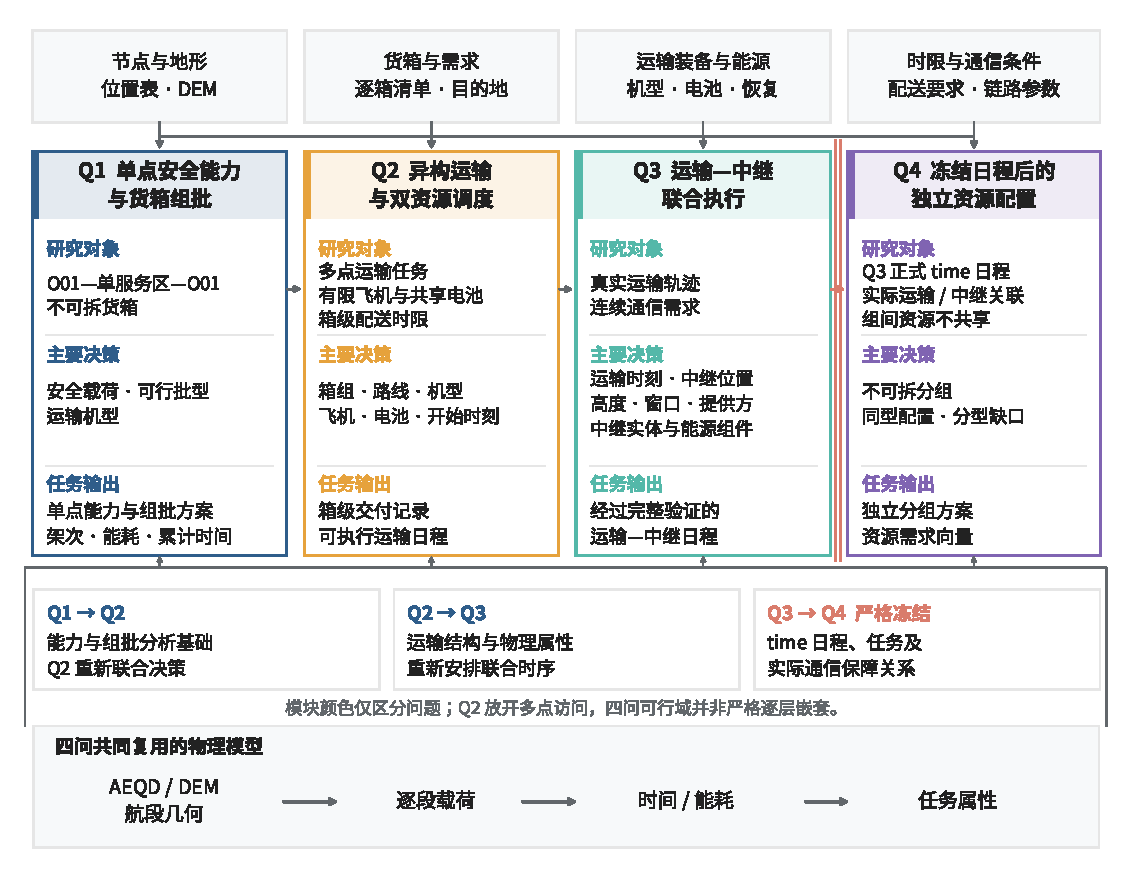
\includegraphics[width=\linewidth]{figures/common_model/fig1_1_decision_inheritance.pdf}
\caption{统一物理模型支撑的四问决策层次与数据继承关系；仅问题三到问题四冻结已选日程}\label{fig:overall_framework}
\end{figure}

稳健性分析贯穿四问，但检验对象不同：问题一关注安全余量和能耗偏差，问题二关注搜索结果分布、充电和作业延迟，问题三关注传播损耗与中继到位时间，问题四关注库存和上游预案。全文将“固定原方案”“固定结构修复时刻”“重新优化结构”分别记录。所用扰动水平是人工压力测试，不被解释为真实灾害条件的概率分布。




\section{模型假设与符号说明}
\label{sec:assumptions_symbols}

\subsection{基本假设}

题目规定的货箱不可拆分、配送时限和通信规则直接作为相应模型的约束。名义模型采用给定参数；稳健性与敏感性试验仅改变各节明确列出的参数，并单独说明允许调整的决策。在此基础上，结合现有数据与计算模型，作如下假设。

\begin{enumerate}[label=\textbf{假设\arabic*.},leftmargin=3.5em]
\item \textbf{输入确定。}以附件给出的节点、物资需求和装备参数进行本轮规划，不另设设备随机故障情景；任务时间与能耗按给定参数计算。
\item \textbf{装载简化。}货箱作为不可拆分单位，仅按总质量和总体积判断装载可行性，不考虑货箱姿态与三维排布；组批结果只确定货箱归属。
\item \textbf{航迹简化。}相邻访问节点采用以O01为中心的WGS84方位等距投影（AEQD）平面直线，地形限制由相交DEM像元确定，不增设未给定的地物、禁飞区或动态障碍物。
\item \textbf{同型资源等效。}同型号无人机、电池及同类中继资源性能一致，可以在类型内部指派复用；不同类型之间不可替代。
\item \textbf{能源独立恢复。}电池与中继能源组件分别按规定充电关系恢复，不另设共享充电设备的容量和排队约束；同一资源未恢复前不得复用。
\end{enumerate}

\subsection{统一计算约定}
\subsubsection{空间、时间与资源释放}
\begin{enumerate}[label=(\arabic*),leftmargin=3.0em]
\item \textbf{空间与能耗。}普通运输采用第3章的地形净空、作业高度和能耗规则：下降计时但不另计下降能耗，空载返航仍计水平与爬升能耗。中继转场与悬停按第6章单独处理，不改写普通运输模型。
\item \textbf{时间与交付。}运输任务以开始准备为相对零时刻，作业时长$p_r$计至返航。送达时刻取所在服务区的交接完成时刻，而非抵达时刻。累计作业时间$T^{\mathrm{sum}}$是各架次时长之和，不是并行执行的最后返航时刻。
\item \textbf{资源占用。}统一采用半开区间$[\mathrm{start},\mathrm{release})$，同刻释放与开始不重复计占用。运输机返航后释放，电池充满后可用，中继机另计规定周转。末次充电保留在能源占用中，但不计入最后返航时间。
\end{enumerate}
\subsubsection{通信条件、评价与数据继承}
\noindent\textbf{通信与分组。}通信采用直连优先、必要时单中继接入与回传共同保障的方式，地形遮挡按第6章处理。问题四固定问题三正式联合方案的任务、绝对时刻、位置及实际保障关系，仅改变服务区分组和组内同型资源指派，组间不共享实体资源。

内部计算统一使用m、s、kg、m$^3$、kWh和dB；比例量按无量纲数计算。分钟、百分数及小数位仅用于展示，模型判定与跨问继承使用未舍入值。各问目标优先关系与局部变量在相应章节定义。

\subsection{主要符号说明}

表\ref{tab:main_symbols}列出公共模型与各问衔接所用的主要符号。下标$i,j$用于节点或路径位置，$b$用于货箱，$m$用于机型，$r$用于运输任务；资源配置中的$g,p$分别表示任务组和资源类型。

\begingroup
\begin{longtable}{@{}p{3.0cm}p{\dimexpr\textwidth-4.8cm-4\tabcolsep\relax}p{1.8cm}@{}}
\caption{主要符号及计量单位}\label{tab:main_symbols}\\
\toprule
\textbf{符号} & \textbf{含义} & \textbf{单位}\\
\midrule
\endfirsthead
\caption[]{主要符号及计量单位（续）}\\
\toprule
\textbf{符号} & \textbf{含义} & \textbf{单位}\\
\midrule
\endhead
\midrule
\multicolumn{3}{r}{\small 接下页}\\
\endfoot
\bottomrule
\endlastfoot
\multicolumn{3}{l}{\textbf{对象与物理量}}\\*
$\mathcal V,\mathcal S$ & 全部空间节点集合、服务区集合，$\mathcal V=\{O01\}\cup\mathcal S$ & --\\
$\mathcal B,\mathcal B_i,\mathcal B_r$ & 全部货箱、服务区$i$的货箱及任务$r$携带的货箱集合 & --\\
$\mathcal M,\mathcal R$ & 机型集合$\{A,B,C\}$、运输任务集合 & --\\
$m_r,\pi_r$ & 任务$r$的机型、有序访问路径 & --\\
$\mu_b,\nu_b$ & 货箱$b$的质量、体积 & kg，m$^3$\\
$Q_m,V_m$ & 机型$m$的额定载荷、货舱体积 & kg，m$^3$\\
$E_m$ & 机型$m$满电电池的可用能量 & kWh\\
$d_{ij}$ & 节点$i$至$j$的水平航段距离 & m\\
$z_i,h_i,H_{ij}$ & 节点地面海拔、作业海拔及航段巡航海拔 & m\\
$q_{r,j}$ & 任务$r$从$v_j$飞往$v_{j+1}$时的实际载荷；$q_{r,0}$为初始载荷 & kg\\
$E_r$ & 运输任务$r$的总能耗 & kWh\\
$\alpha_m,SOC_r^{\mathrm{return}}$ & 机型$m$的返航安全余量、任务$r$的返航荷电状态 & --\\
\midrule
\multicolumn{3}{l}{\textbf{时间与配送}}\\*
$s_r,p_r$ & 任务$r$的绝对开始时刻、从准备至返航的作业时长 & s\\
$c_r$ & 任务$r$返航后对应电池充至满电的恢复时长 & s\\
$\delta_{rb},C_b$ & 货箱$b$的相对交接完成偏移、绝对送达时刻，$C_b=s_r+\delta_{rb}$ & s\\
$d_b,h_b$ & 货箱$b$的期望送达时刻、硬截止时刻；后者仅对有硬时限的货箱定义 & s\\
$\omega_b,L_w$ & 货箱优先权重、全部货箱的加权迟到 & --，s\\
$T^{\mathrm{sum}}$ & 运输架次累计作业时间，$\sum_{r\in\mathcal R}p_r$ & s\\
$T_{\max}$ & 全部运输任务的最后返航时刻 & s\\
$T_{\max}^{joint}$ & 全部运输与中继任务的联合最后返航时刻 & s\\
\midrule
\multicolumn{3}{l}{\textbf{通信与资源配置}}\\*
$L_{ab}(t),L_{ab}^{\max}$ & 通信端点$a,b$间的传播损耗、允许传播损耗上限 & dB\\
$\Delta$ & 统一增加的传播损耗 & dB\\
$\mathcal P,I_{jp}$ & 资源类型集合、固定任务$j$对资源类型$p$的占用区间 & --，s\\
$N_{gp}^{\min}$ & 任务组$g$独立执行所需的$p$类资源最小数量 & 个\\
$I_p,D_p,G_p$ & $p$类资源的现有库存、独立分组后总需求及正缺口 & 个\\
\end{longtable}
\endgroup

表中“--”表示集合、标识或无量纲量。通信端点$a,b$与货箱下标$b$分别在各自语境中使用；资源配置中任务下标$j$不表示运输路径的第$j$站。




\section{数据处理与公共物理模型}
\label{sec:foundation}

各问首先都需要判断一项运输任务是否能飞，以及执行它需要多少时间和能量。本章将节点、货箱、装备和地形数据转换为统一任务属性。后续改变的是任务组合、资源时序与组织方式，而不是在不同问题中任意改用另一套距离或能耗公式。

\subsection{输入数据整理与一致性检查}
\subsubsection{节点、货箱与装备数据关联}
位置表以节点编号关联，逐箱清单以货箱编号唯一标识。将同一服务区、同一物资类型的箱数汇总后与需求汇总表核对，避免重复计入汇总需求和明细需求。整理结果为1个基地O01、15个服务区和80箱物资，总质量758\,kg、总体积2.011\,m$^3$。记服务区集合为$\mathcal S$，空间节点集合为$\mathcal V=\{O01\}\cup\mathcal S$，货箱集合为$\mathcal B$。

节点$i$保留原表经纬度$(\lambda_i,\varphi_i)$与地面高程$z_i$；货箱$b$记录目的地$s(b)$、质量$\mu_b$和体积$\nu_b$。配送时限和优先权重在问题二以后进入调度评价，不参与问题一的静态组批。图\ref{fig:scene}展示位置与需求，点面积表示质量，不表示灾情严重程度。
\begin{figure}[htbp]\centering
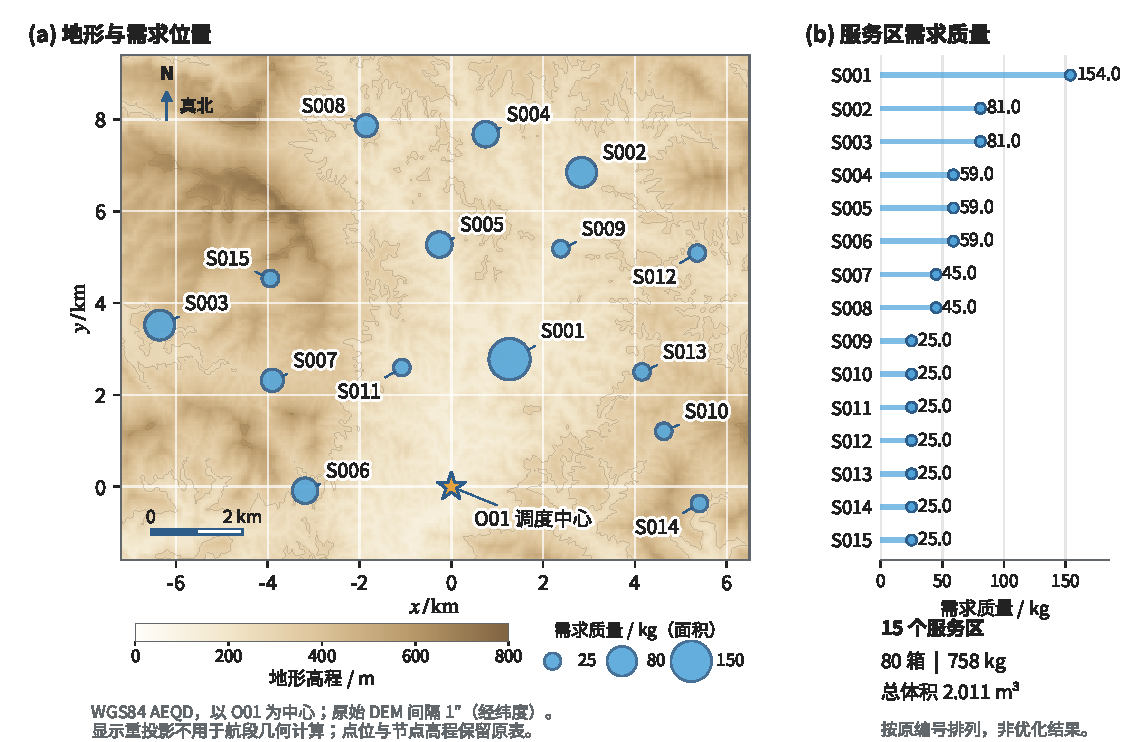
\includegraphics[width=\linewidth]{figures/common_model/fig3_1_terrain_and_demand.pdf}
\caption{救援区域地形与不可拆物资需求。显示重投影不参与航段计算，点面积与需求质量成正比}\label{fig:scene}
\end{figure}

机型参数见表\ref{tab:common_drone}。含电池空载质量、额定载荷和电池可用能量分别参与不同公式，不能混为有效载重。准备、装载、交接、升降速度和爬升效率同样按机型读取。
\begin{table}[htbp]\centering\small
\caption{三类运输无人机主要物理参数}\label{tab:common_drone}
\begin{tabular}{lrrr}\toprule 参数 & A型 & B型 & C型\\\midrule
含电池空载质量/kg &70&65&69.9\\
额定载荷/kg &25&30&80\\
货舱体积/m$^3$ &0.060&0.073&0.250\\
巡航速度/(m/s)&12&15&15\\
空载航程/m&25000&28000&26000\\
满载航程/m&20000&16000&12000\\
可用电池能量/kWh&4.5&4.0&8.0\\
基准返航安全余量&20\%&20\%&20\%\\\bottomrule
\end{tabular}
\end{table}


\subsubsection{需求结构与机型容量的对应}
逐箱聚合如表\ref{tab:rev_cargo}。不同物资的质量与体积占比并不相同：饮用水构成主要质量负担，生活卫生用品则具有较高的单位质量体积。医疗物资的质量较小，但其硬截止对任务顺序具有直接影响。因此本文独立保留质量、体积和时限三个维度，不用平均货物密度或平均期限合并。

\begin{table}[htbp]\centering\small
\caption{逐箱需求的类型结构与容量规模}\label{tab:rev_cargo}
\begin{tabular}{lrrrr}\toprule
物资类型 & 箱数 & 质量/kg & 体积/m$^3$ & 质量占比/\%\\\midrule
医疗物资 & 16 & 48 & 0.192 & 6.33\\
应急食品 & 19 & 152 & 0.532 & 20.05\\
饮用水 & 36 & 504 & 0.972 & 66.49\\
生活卫生用品 & 9 & 54 & 0.315 & 7.12\\
\bottomrule\end{tabular}
\end{table}


为识别一个候选箱组首先触发的限制，定义容量占用比
\begin{equation}
 \rho_{rm}^{Q}=\frac{\sum_{b\in\mathcal B_r}\mu_b}{Q_m},\quad
 \rho_{rm}^{V}=\frac{\sum_{b\in\mathcal B_r}\nu_b}{V_m},\quad
 \rho_{rm}^{E}=\frac{E_r}{(1-\alpha_m)E_m}.
 \label{eq:dimensionless_capacity}
\end{equation}
三个比值均不大于1才满足当前任务的相应约束。$\rho^V$较大时应优先考虑货舱匹配；$\rho^E$较大时，瓶颈来自航段和载荷能耗；$\rho^Q$较大则反映额定质量接近上限。占用比用于解释约束，不替代原始单位下的可行性计算。

数据关联分别核对编号、量纲与总量守恒。每个箱号只能对应一个目的地和一套原始属性，所用目的地与机型必须存在于输入表中；组批及路线调整后，原始箱号全集、758 kg质量与2.011 m$^3$体积保持不变。优化改变的是任务组合与执行时序，不改变需求记录本身。


\subsubsection{地形数据及空间坐标转换}
TIF与MAT两种地形文件分别核对高程矩阵、像元中心坐标和仿射边界。模型直接在原始栅格上计算航段经过地形，不用平滑或重采样改变山体。节点高程仍使用位置表值，不能用邻近DEM值悄然替换。地形显示与计算使用不同副本，显示分辨率不改变物理判定。

以O01为中心建立WGS84方位等距投影（AEQD）\cite{snyder1987}。令$\boldsymbol x_i=(x_i,y_i)^{\mathsf T}$，则
\begin{equation}
\boldsymbol x_i=\operatorname{AEQD}_{O01}(\lambda_i,\varphi_i),\qquad
 d_{ij}=\|\boldsymbol x_j-\boldsymbol x_i\|_2.
\label{eq:common_projection}
\end{equation}
任意访问节点间的水平航迹规定为投影平面直线：
\begin{equation}
\boldsymbol r_{ij}(u)=(1-u)\boldsymbol x_i+u\boldsymbol x_j,\qquad 0\le u\le1.
\label{eq:common_planar_path}
\end{equation}
以O01为端点的径向航段可用椭球测地线独立核验；这不意味着任意服务区间的投影距离都等于测地线距离。求与地形栅格的相交时，需要连续反投影式\eqref{eq:common_planar_path}，不能对经纬度端点直接线性插值代替。

\subsection{地形约束下的航段几何}
\subsubsection{航迹与地形像元的完整相交}
原始GeoTIFF采用像元中心定位。设左上参考像元中心为$(\lambda_c,\varphi_c)$，角度间隔为$\Delta\lambda,\Delta\varphi>0$，则栅格左上边界为
\begin{equation}
\lambda_0=\lambda_c-\tfrac12\Delta\lambda,\qquad
\varphi_0=\varphi_c+\tfrac12\Delta\varphi.
\label{eq:common_half_pixel}
\end{equation}
反投影航迹$(\lambda(u),\varphi(u))$对应连续列、行坐标
\begin{equation}
\xi(u)=\frac{\lambda(u)-\lambda_0}{\Delta\lambda},\qquad
\eta(u)=\frac{\varphi_0-\varphi(u)}{\Delta\varphi}.
\label{eq:common_raster_coordinates}
\end{equation}
半像元校正用于对应TIF中心定位与MAT边界变换，不是人为移动航迹。求出轨迹与整数行列边界的交点并按$u$排序；相邻交点之间没有新的栅格边界，检查其中点及全部交点即可得到相交像元集合$\mathcal C_{ij}$。采用闭像元约定，格边与角点接触的所有像元均计入。

问题一的径向航段在核实坐标单调性后逐边界求根，这一处理不外推到任意非单调长轨迹。超出DEM范围或经过无效高程时拒绝该几何输入，不以零高程填补。固定步长采样可以用于显示与对照，但不能保证发现短暂接触的每个像元。


\subsubsection{几何事件分割与计算缓存}
AEQD线段、反投影航迹和原始DEM分别承担平面路径定义、栅格定位和地形查询。对于基地径向距离，使用椭球测地线作为独立核验对象，相关数值算法可参照Karney\cite{karney2013}。显示地图的重采样不进入能耗和高度计算，保证图形美化不会改变模型。

设一条航迹的格边交点参数及两个端点排序为
\begin{equation}
0=u_0<u_1<\cdots<u_M=1.
\label{eq:geometry_breakpoints}
\end{equation}
在相邻事件之间没有新的格边穿越，其所在像元集合不变。因此每个开区间用内部点定位，同时对交点采用闭像元约定，即可覆盖连续路径实际触及的像元。边界和角点接触不能只由两端采样点推断；完整事件分割正是地形核验的重要步骤。

对固定有向航段缓存水平距离、最高地形、巡航海拔、端点作业高度和升降高度。反向航段可以共享距离和最高地形，但升降高度按起终点重新计算。改变箱组而路线不变时复用几何，重新计算载荷能耗；改变访问顺序则读取新的有向航段；中继位置或悬停高度改变后，转场与通信几何均需更新。这种分层复用减少重复地形查询，又保持候选之间相同的物理口径。


\subsubsection{巡航海拔、作业高度与飞行阶段}
设$Z_c$为像元高程，普通运输的航段最高地形、巡航海拔及作业高度为
\begin{equation}
 z_{ij}^{\max}=\max_{c\in\mathcal C_{ij}}Z_c,\qquad H_{ij}=z_{ij}^{\max}+50,
\label{eq:common_cruise_altitude}
\end{equation}
\begin{equation}
 h_i=\begin{cases}z_i,&i=O01,\\z_i+30,&i\in\mathcal S,\end{cases}
 \quad h_{ij}^{\uparrow}=H_{ij}-h_i,\quad h_{ij}^{\downarrow}=H_{ij}-h_j.
\label{eq:common_work_height}
\end{equation}
每段均经历爬升、巡航和下降。完成服务区交接后，下一段从该区作业高度重新起算，空载返航也可能再次爬升。计算前检查$H_{ij}\ge\max(h_i,h_j)$；若不成立，应报告高度口径冲突，不能把负爬升直接截为零。中继悬停端点可能高于该巡航面，第\ref{sec:q3}章单独定义中继转场规则，不反向修改普通运输模型。

\begin{figure}[htbp]\centering
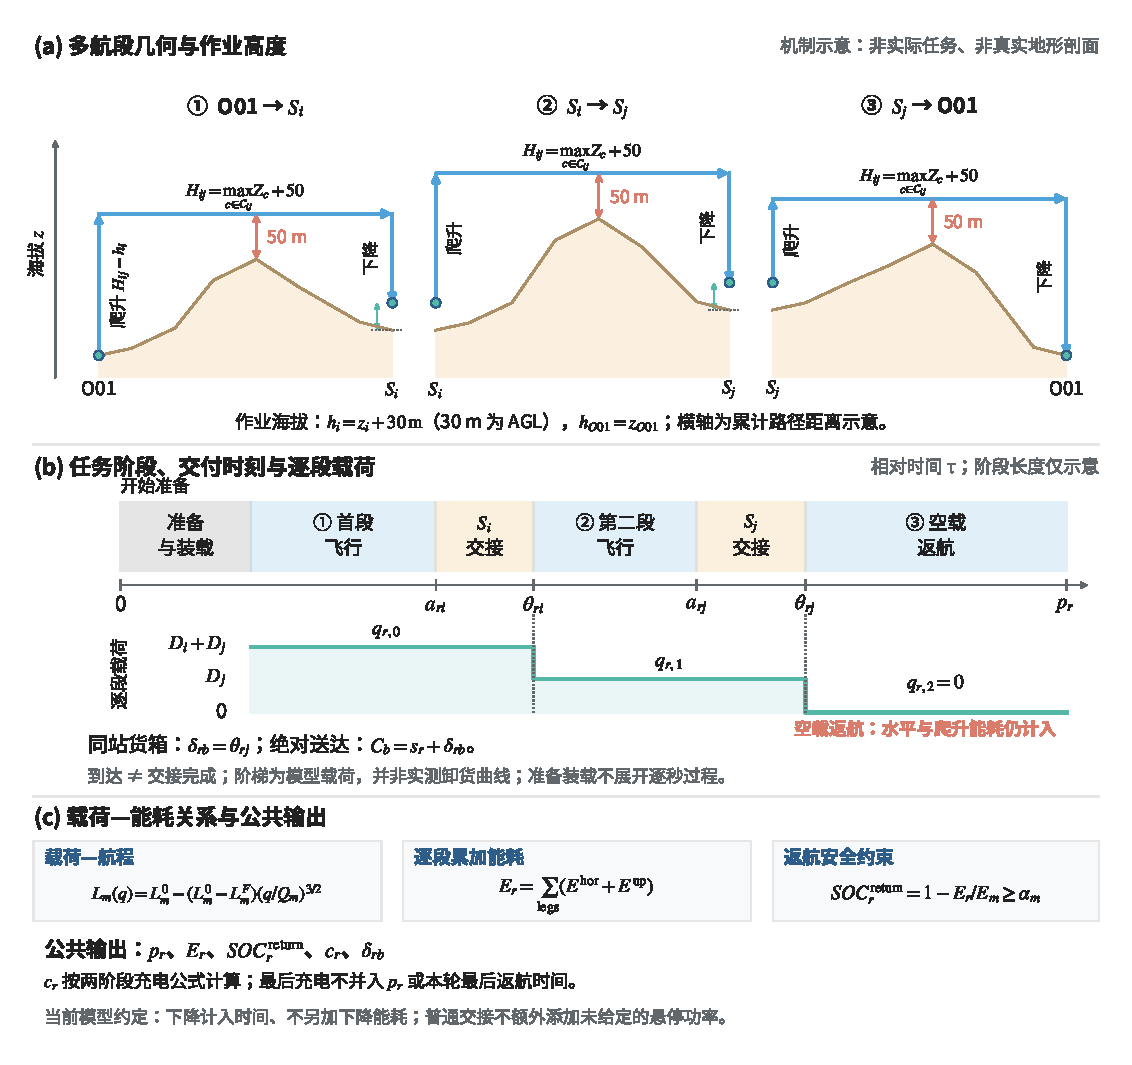
\includegraphics[width=\linewidth]{figures/common_model/fig3_2_transport_physics.pdf}
\caption{多点运输的航段几何、离站载荷、交接完成与能耗计算机制（示意）；距离轴与时间轴不同}\label{fig:common_leg_geometry}
\end{figure}

\subsection{运输任务的载荷与时间计算}
\subsubsection{任务组成与逐站卸货}
一项任务表示为$r=(m_r,\mathcal B_r,\pi_r)$，其中机型$m_r\in\{A,B,C\}$，箱组为$\mathcal B_r$，有序路线$\pi_r=(v_0,v_1,\ldots,v_K,v_{K+1})$满足$v_0=v_{K+1}=O01$。中间节点与箱组目的地一致，当前任务构造不重复访问同一服务区。第$j$站交付数量与质量为
\begin{equation}
 n_{rj}=|\{b\in\mathcal B_r:s(b)=v_j\}|,\qquad
 D_{rj}=\sum_{\substack{b\in\mathcal B_r\\s(b)=v_j}}\mu_b.
\label{eq:common_drop}
\end{equation}
起飞容量与逐站载荷满足
\begin{equation}
 q_{r,0}=\sum_{b\in\mathcal B_r}\mu_b\le Q_{m_r},\qquad
 \sum_{b\in\mathcal B_r}\nu_b\le V_{m_r},
\label{eq:common_capacity}
\end{equation}
\begin{equation}
 q_{r,j}=q_{r,j-1}-D_{rj},\qquad q_{r,0}\ge\cdots\ge q_{r,K}=0.
\label{eq:common_load}
\end{equation}
$v_j\to v_{j+1}$使用$q_{r,j}$计算，包括$j=K$的空载返航。途中只卸货、不补货，故初始容量合格后质量与体积不再增加；但能耗必须按卸货后的各段载荷计算。改变访问顺序会改变高载荷飞行距离，不能只比较总路程。

\subsubsection{交接完成时刻与返航时间}
设爬升、巡航、下降速度为$v_m^\uparrow,v_m^c,v_m^\downarrow$，则
\begin{equation}
 t_{ij}^{\mathrm{fly}}(m)=\frac{h_{ij}^{\uparrow}}{v_m^{\uparrow}}+\frac{d_{ij}}{v_m^c}+\frac{h_{ij}^{\downarrow}}{v_m^{\downarrow}}.
\label{eq:common_leg_time}
\end{equation}
以开始准备为任务相对零时刻。固定准备、单箱装载、每站基础交接和单箱交接时间分别为$t_m^{\mathrm{prep}},t_m^{\mathrm{load}},t_m^{\mathrm{hand}},t_m^{\mathrm{box}}$。令$n_r=|\mathcal B_r|$，起飞时刻$\theta_{r,0}=t_{m_r}^{\mathrm{prep}}+n_rt_{m_r}^{\mathrm{load}}$。到达与交接完成时间依次为
\begin{equation}
\begin{aligned}
 a_{r,j}&=\theta_{r,j-1}+t_{v_{j-1}v_j}^{\mathrm{fly}}(m_r),\\
 \theta_{r,j}&=a_{r,j}+t_{m_r}^{\mathrm{hand}}+n_{rj}t_{m_r}^{\mathrm{box}},\quad j=1,\ldots,K.
\end{aligned}
\label{eq:common_delivery_recursion}
\end{equation}
货箱以\emph{交接完成}而非抵达作为送达时刻；同站货箱共享该交接完成时刻。若$b$在第$j$站交付，则$\delta_{rb}=\theta_{r,j}$，绝对开始时刻为$s_r$时有
\begin{equation}
 C_b=s_r+\delta_{rb},\qquad p_r=\theta_{r,K}+t_{v_KO01}^{\mathrm{fly}}(m_r).
\label{eq:common_delivery_return}
\end{equation}
展开得到
\begin{equation}
\begin{split}
 p_r={}&t_{m_r}^{\mathrm{prep}}+n_rt_{m_r}^{\mathrm{load}}
 +\sum_{j=0}^Kt_{v_jv_{j+1}}^{\mathrm{fly}}(m_r)\\
 &+\sum_{j=1}^K\bigl(t_{m_r}^{\mathrm{hand}}+n_{rj}t_{m_r}^{\mathrm{box}}\bigr).
\end{split}
\label{eq:common_task_duration}
\end{equation}
该递推同时输出每箱交付偏移和返航时间，不需要按总时长平均分摊。问题一用$T^{\mathrm{sum}}=\sum_rp_r$衡量累计工作量；并行调度用$T_{\max}=\max_r(s_r+p_r)$衡量最后返航时刻。二者不能替代。

\subsection{能耗计算与返航安全约束}
\subsubsection{载荷相关航程与分阶段能耗}
配送能耗需要考虑载荷与任务组织\cite{zhang2021energy,zhang2023corrigendum}。具体计算沿用题面给定关系，不拟合其他型号的功率曲线。对$0\le q\le Q_m$，等效航程为
\begin{equation}
 L_m(q)=L_m^0-(L_m^0-L_m^F)\left(\frac q{Q_m}\right)^{3/2}.
\label{eq:common_range}
\end{equation}
该量是水平能耗的标定长度，不是一次往返可到达的单程半径。水平与爬升能耗分别为
\begin{equation}
 E_m^{\mathrm{hor}}(d,q)=E_m\frac d{L_m(q)},\qquad
 E_m^{\mathrm{up}}(q,h)=\frac{(m_m^0+q)gh}{\eta_m\,3.6\times10^6}.
\label{eq:common_energy_parts}
\end{equation}
$m_m^0$包含电池质量，$\eta_m$为爬升效率，$g=9.81\,\mathrm{m/s^2}$；焦耳除以$3.6\times10^6$转换为kWh。当前参数化中，下降计时但不另加能耗；普通交接不额外添加未给定的悬停功率。中继长时间悬停由第\ref{sec:q3}章单独计算。这是模型约定，不是对实际下降或交接能量的普遍断言。

\subsubsection{任务总能耗与返航剩余电量}
按实际逐段载荷求和：
\begin{equation}
 E_r=\sum_{j=0}^{K}\left[
 E_{m_r}\frac{d_{v_jv_{j+1}}}{L_{m_r}(q_{r,j})}
 +\frac{(m_{m_r}^0+q_{r,j})g\,h_{v_jv_{j+1}}^{\uparrow}}{\eta_{m_r}\,3.6\times10^6}\right].
\label{eq:common_task_energy}
\end{equation}
最后一段$q_{r,K}=0$，但水平飞行和空载爬升项仍然存在。每次任务使用满电电池时，返航安全判据为
\begin{equation}
 E_r\le(1-\alpha_{m_r})E_{m_r},\qquad
 SOC_r^{\mathrm{return}}=1-\frac{E_r}{E_{m_r}}\ge\alpha_{m_r}.
\label{eq:common_reserve}
\end{equation}
基准$\alpha_m=0.20$。式\eqref{eq:common_capacity}与\eqref{eq:common_reserve}共同决定物理可行性。它们本身不保证有限资源排程或连续通信可行。


\subsubsection{载荷的边际能耗与安全边界}
记$a_m=L_m^0-L_m^F>0$。在$q>0$时，给定航程公式有
\begin{equation}
L'_m(q)=-\frac{3a_m}{2Q_m^{3/2}}\sqrt q<0,\qquad
\frac{\partial E_m^{\mathrm{hor}}}{\partial q}
=-\frac{E_m dL'_m(q)}{L_m(q)^2}>0.
\label{eq:energy_load_derivative}
\end{equation}
爬升能耗对载荷的导数为$gh/(\eta_m3.6\times10^6)$，亦不小于0。因此固定机型和航段后，增加离站载荷不会降低能耗。单点往返中返程为空载，边界求根只需处理起飞载荷对去程的影响。

此外，$L''_m(q)<0$，从而
\begin{equation}
\frac{\partial^2 E_m^{\mathrm{hor}}}{\partial q^2}
=E_md\left[\frac{2(L'_m)^2}{L_m^3}-\frac{L''_m}{L_m^2}\right]>0.
\label{eq:energy_load_convexity}
\end{equation}
高载荷区间具有更高的边际水平能耗，这解释了把货箱从重载任务移至较轻任务可能产生节能。然而新增任务也引入准备、交接、空载返航和额外爬升，故不能仅按载荷均衡确定组批。后文在完整任务成本上评价这种权衡。

当安全能量约束决定最大载荷时，对$E_{im}(w)=(1-\alpha)E_m$求导得到
\begin{equation}
\frac{\mathrm d w_{im}^{safe}}{\mathrm d\alpha}
=-\frac{E_m}{\partial E_{im}/\partial w}<0.
\label{eq:payload_alpha_derivative}
\end{equation}
当额定质量先起作用，安全载荷曲线保持平台；能量边界降至额定质量以下才开始下降。这给出了第四章载荷曲线“平台—下降”结构的模型解释。

本文的$E_r$是给定模型下的任务电池能耗。Stolaroff等的生命周期研究还涉及供电来源和物流系统边界\cite{stolaroff2018,stolaroff2018corr}。本题使用任务能耗直接计算返航余量与恢复时间，相关节能结果按这一明确单位和范围报告。


\subsection{能源恢复与资源占用}
\subsubsection{两阶段充电恢复时间}
设完全充电等效时间为$\tau^{\mathrm{full}}$，任务结束荷电状态为$\rho$。从0充至90\%占完全充电时间65\%，90\%至100\%占35\%，故
\begin{equation}
 \tau(\rho)=\tau^{\mathrm{full}}\begin{cases}
 0.65(0.9-\rho)/0.9+0.35,&0\le\rho<0.9,\\
 0.35(1-\rho)/0.1,&0.9\le\rho\le1.
 \end{cases}
\label{eq:common_recharge}
\end{equation}
在$\rho=0,0.9,1$处分别得到$\tau^{\mathrm{full}}$、$0.35\tau^{\mathrm{full}}$、0，且90\%处连续。该函数不能简化为“耗电比例乘完全充电时间”。充电敏感性试验统一缩放$\tau^{\mathrm{full}}$，仍保留上述两段比例。

\subsubsection{飞机、电池与中继资源的释放区别}
令$c_r=\tau(SOC_r^{\mathrm{return}})$，从任务开始准备起，运输飞机与电池分别占用
\begin{equation}
 I_r^U=[s_r,s_r+p_r),\qquad I_r^B=[s_r,s_r+p_r+c_r).
\label{eq:common_occupancy}
\end{equation}
运输机返航后释放，原电池须充满才能再用；末次充电不计入最后返航时间，但仍计入能源占用。中继实体还有规定的返航周转，其释放不能直接套用$I_r^U$。各区间使用原始精度；同刻释放与开始允许衔接，不能先舍入分钟再计算资源峰值。


\subsubsection{充电恢复对能源偏差的响应}
令放电比例$e=E_r/E_m$，两阶段恢复函数可等价改写为
\begin{equation}
 c(e)=\tau^{\mathrm{full}}
 \begin{cases}
 3.5e,&0\le e\le0.1,\\
 \dfrac{13}{18}e+\dfrac5{18},&0.1<e\le1.
 \end{cases}
\label{eq:charge_energy_fraction}
\end{equation}
两段在$e=0.1$均等于$0.35\tau^{\mathrm{full}}$，恢复时间随耗电单调增加。慢充末段每单位充电量需要更多时间，因而恢复时长不宜用“耗电比例乘完全充电时间”代替。

若统一能耗偏差为$\varepsilon$，且扰动前后处于相同充电分段，则
\begin{equation}
 \Delta c_r=\tau_m^{\mathrm{full}}\kappa_r\frac{E_r}{E_m}\varepsilon,
 \qquad \kappa_r\in\{3.5,13/18\}.
\label{eq:charge_local_perturbation}
\end{equation}
能源偏差由此转化为可用时刻偏差。即使返航SOC仍满足下限，只要前后任务之间没有足够的电池接续余量，原日程也可能需要修复。这正是第五章分别检查能量与时间接续的原因。

\subsubsection{完整单点任务的计算链示例}
S006的C型任务携带6箱、59 kg、0.156 m$^3$。准备与装载共$300+6\times30=480$ s，交接共$180+6\times36=396$ s。从完整任务1561.553868 s中扣除两项，往返飞行为685.553868 s，三部分之和返回原任务时长。

其能耗2.597987865 kWh，返航SOC为67.525152\%。根据式\eqref{eq:charge_energy_fraction}，在完全充电时间3000 s下，恢复时长为1536.955047 s。任务若在$s$开始，飞机于$s+1561.553868$释放，电池约于$s+3098.508915$恢复。这个单任务算例连接了箱组、飞行、交付、能源和资源释放，也为后续敏感性重放提供统一计算顺序。

资源调度研究把容量、占用和先后关系作为可扩展的结构要素\cite{hartmann2022}。本题将飞机和电池建为可分离资源池，允许返航飞机使用另一组已满电的兼容电池；因此增配电池能缓解恢复等待，但不能突破飞机总工作量下界。后续用日程和瓶颈分析分别识别这两类限制。


\subsection{公共模型核验}
\subsubsection{几何与单任务计算核对}
先检查$L_m(0)=L_m^0$、$L_m(Q_m)=L_m^F$、完整交付后$q_{r,K}=0$，再逐项核对时间、交付偏移、SOC及充电分段连续性。以S006的C型单点任务为例，6箱共59\,kg、0.156\,m$^3$，能耗2.597987865\,kWh、作业时长1561.553868\,s。代回8\,kWh电池容量得到返航SOC为67.525152\%，恢复时长为$0.512318349\tau_C^{\mathrm{full}}$。本例只检查任务属性，未把单架次可行误写成系统排程可行。

已有几何核验对15条基地径向航段使用独立测地线和像元条带求交：距离最大差为$1.412\times10^{-9}$\,m，相交集合一致；0.25\,m固定采样对照合计漏过4个相交像元。这说明完整相交优于该采样对照，但不构成任意服务区间投影误差的上界，也不能识别DEM分辨率以下的障碍物。本轮进一步从原始任务属性重算问题二23个架次及80箱交付，与保存计划在$10^{-6}$\,s和$10^{-7}$\,kWh范围内对应。

\subsubsection{任务输出与后续模型接口}
公共计算将任务转换为机型、箱组、路线、载荷序列、$p_r,E_r,SOC_r,c_r$和$\delta_{rb}$。问题一在此基础上选择可行批型，问题二加入有限飞机、电池及配送时限，问题三使用分段三维轨迹检查通信，问题四冻结运输与中继的实际占用区间。

对于敏感性计算，输入扰动必须进入相关物理项，而非直接放大结果工期。例如能耗增加会同时改变SOC与充电时间；交接延迟改变后续交付和返航，但在当前无额外交接功率的模型中不自动增加能耗。本文分别保留名义计算、固定决策重放和允许调整后的结果，避免把不同实验权限混为一个“通过率”。


\section{问题一：安全运输能力与货箱组批}
\label{sec:q1}

\subsection{问题分析与求解思路}
\subsubsection{单点往返的运输能力限制}
本问每个架次只执行$O01\to S_i\to O01$，不跨服务区组批，也不决定实体飞机和电池的并行日程。需要先回答同一机型面对不同地形与航程能安全携带多少质量，再决定完整货箱如何组合。额定载荷只是一个上限，不能忽略空载返航的能量需求后直接作为安全载荷。

\subsubsection{从安全载荷到离散组批}
先计算15个服务区与3类机型的45组安全载荷，再在各区枚举非空货箱组合，筛去质量、体积或能量不合格的组合。可行组合构成有限批型集，后续选择批型使每箱恰好运输一次。本文先最少架次，再比较能耗，最后比较累计作业时间；另保留不同目标向量的非支配方案，使优先关系可见而不依赖任意权重。

\subsection{安全载荷与组批模型}
\subsubsection{最大安全载荷计算}
对服务区$i$与机型$m$，记携带质量$w$的完整往返能耗为$E_{im}(w)$。安全载荷定义为
\begin{equation}
 w_{im}^{\mathrm{safe}}=\max\{w\in[0,Q_m]:E_{im}(w)\le(1-\alpha_m)E_m\}.
\label{eq:q1_safe_payload}
\end{equation}
在给定模型中，载荷增加使等效航程下降，水平和爬升能耗均不减。先检查额定载荷；额定载荷不满足而空载可行时，对边界方程$E_{im}(w)=(1-\alpha_m)E_m$求根。空载亦不可行时该组合没有可用运输能力，而不是将不成立的根强行赋为零。保存结果以Brent法与独立二分法核对。

基准20\%余量下，45项中39项达到额定质量，6项先受能量限制。图\ref{fig:q1_payload}以颜色表示额定能力保留比例，格内给出公斤数，避免将大机型的绝对载荷与相对折减混淆。S008的B、C型安全载荷分别为28.801、58.904\,kg；C型额定80\,kg不能直接用于该区。
\fig[.78]{q1_payload.pdf}{20\%返航安全余量下的最大安全载荷。格内为kg，颜色为安全载荷与额定载荷之比；描框项受到能量限制。}{fig:q1_payload}

\subsubsection{可行货箱组合与完整配送约束}
对服务区$i$的箱集$\mathcal B_i$，任一非空子集$S\subseteq\mathcal B_i$与机型$m$若满足
\begin{equation}
 \sum_{b\in S}\mu_b\le Q_m,\qquad
 \sum_{b\in S}\nu_b\le V_m,\qquad
 E_{im}\!\left(\sum_{b\in S}\mu_b\right)\le(1-\alpha_m)E_m,
\label{eq:q1_pattern_feasibility}
\end{equation}
则形成可行批型$p=(i,m,S)$，其能耗和作业时间为$E_p,T_p$。记全集$\mathcal P=\bigcup_i\mathcal P_i$，变量$y_p\in\{0,1\}$表示是否采用该批型，完整配送要求
\begin{equation}
 \sum_{p:b\in S_p}y_p=1,\qquad \forall b\in\mathcal B.
\label{eq:q1_cover}
\end{equation}
每箱恰好被一个批型覆盖，同时禁止跨服务区组合。质量安全载荷只辅助理解能力边界；生成批型时仍独立检查体积和完整能耗。

\subsubsection{架次、能耗与累计时间的比较顺序}
选择的目标为
\begin{equation}
 \min_{\mathrm{lex}}\left(N,E,T^{\mathrm{sum}}\right)
 =\min_{\mathrm{lex}}\left(\sum_py_p,\sum_pE_py_p,\sum_pT_py_p\right).
\label{eq:q1_objective}
\end{equation}
实现时先求$N^*$，固定$N=N^*$后求最低能耗，再固定前两项求累计时间。该顺序是本文明确采用的决策偏好；不能因此声称题目只有这一种多目标解释。非支配方案用于说明改变偏好会带来什么代价。


\subsubsection{按服务区分解的等价性}
问题一禁止跨区组批，且不计实体并行与电池接续，故不同服务区之间没有共享时序约束。设各区可行组批集合为$\mathcal X_i$，则
\begin{equation}
\mathcal X=\mathcal X_1\times\cdots\times\mathcal X_{15},\qquad
(N,E,T^{\mathrm{sum}})=\sum_i(N_i,E_i,T_i).
\label{eq:q1_separable}
\end{equation}
若一个全局最少架次方案在某区使用了多于局部最少的架次数，用该区局部最少方案替换即可减少总架次且不影响其他区，产生矛盾。因此$N^*=\sum_iN_i^*$。固定各区最少架次后，同样的替换论证适用于能耗；最后固定前两层，累计时间也可逐区最小化。

这种分解来自约束可分离性，而非启发式近似。问题二允许跨区并使用有限实体，任务之间出现资源耦合，因而不再具有式\eqref{eq:q1_separable}的乘积结构。

\subsubsection{容量下界与候选筛选}
对需求质量$M_i$、体积$V_i^{dem}$，可构造必要下界
\begin{equation}
N_i\ge\max\left\{1,\left\lceil\frac{M_i}{Q^{max}}\right\rceil,
\left\lceil\frac{V_i^{dem}}{V^{max}}\right\rceil\right\}.
\label{eq:q1_capacity_lower}
\end{equation}
质量分母还可替换为该区全部机型安全载荷的最大值。质量界与体积界分别是必要条件，其最大值仍有效；是否达到它则由实际不可拆货箱覆盖决定。S001、S002和S003超过80 kg形成三项两架次下界，其余12区至少一架次，总下界为18。

候选筛选依次检查目的地与箱号、质量与体积、完整任务能源。便宜的组合条件先执行，避免对必定超载的箱组重复查询物理代价。在同一区域同一机型下，增加箱子只会增加质量、体积和给定单调能耗，因此已经超限的组合不能通过继续加箱恢复。筛选后保留原箱号，以便从计数解恢复完整配送清单。


\subsection{精确求解方法}
\subsubsection{原始货箱模型与等价货箱压缩}
箱级整数模型直接对原始箱号生成批型，适合核对完整配送。若同区货箱在质量、体积和本问相关属性上完全一致，箱号置换不改变物理可行性与目标，可用每类箱数压缩对称性。压缩只减少重复代表，并未把不可拆箱改成可连续分割的质量。求得计数方案后再恢复唯一箱号，检查80箱无遗漏和重复。

\subsubsection{剩余需求状态的动态规划}
将某区各等价货箱类别的剩余数量记为$\boldsymbol n=(n_1,\ldots,n_K)$，批型$p$携带计数向量$\boldsymbol c_p$。递推为
\begin{equation}
 F(\boldsymbol n)=\min_{\substack{p:\boldsymbol c_p\le\boldsymbol n}}^{\mathrm{lex}}
 \left\{F(\boldsymbol n-\boldsymbol c_p)+(1,E_p,T_p)\right\},\qquad F(\boldsymbol0)=(0,0,0).
\label{eq:q1_dp}
\end{equation}
每次至少减少一个箱子，状态按剩余总数递增计算，不存在循环。不同服务区互不共享批型且目标可加，总体词典序解由各区最优结果相加得到。需要Pareto集合时，每个状态保留未被架次、能耗、时间三项同时支配的标签，再逐区合并并删除支配标签。


\subsubsection{递推顺序、支配筛选与原箱号恢复}
某区有$K_i$个等价类，需求计数为$d_{ik}$，计数状态数量为
\begin{equation}
|\mathcal N_i|=\prod_{k=1}^{K_i}(d_{ik}+1).
\label{eq:q1_dp_states}
\end{equation}
每个非空批型至少减少一箱，故按箱数递增计算状态时，前驱已经处理。原点为$(0,0,0)$，不可达状态保持空标记，不能被默认填成零成本。直接枚举状态与批型的实现时间为$O(|\mathcal N_i||\mathcal P_i|)$，单目标词典序标签及前驱需要$O(|\mathcal N_i|)$存储。

每次更新同时保存前驱状态和所选批型。最终从完整需求状态回溯，获得机型和计数批型；再从相应等价类的原始箱号池中取出对应数量，恢复唯一箱号。恢复后按原质量、体积和完整往返能耗重新核验，计数压缩不会把货箱变成可分割的连续质量。

多目标递推中只在相同剩余需求状态内比较支配关系。若标签$u$在架次、能耗、时间均不大于$v$，则它们接上相同后续批型后仍保持支配，故$v$可删除；剩余需求不同的状态不能这样互相删除。各区标签集再逐次求和并筛除支配目标。Bouman等在无人机路径研究中使用动态规划压缩重复决策\cite{bouman2018}，本文采用的状态则直接对应本题的不可拆需求计数。

\begin{table}[htbp]\centering\small
\caption{精确组批递推与方案恢复步骤}\label{tab:dp_execution}
\begin{tabularx}{\linewidth}{p{1.5cm}L}\toprule
阶段 & 操作\\\midrule
输入 & 读取等价类需求及质量、体积、能源均合格的计数批型。\\
初始化 & 原点赋零标签，其他状态不可达；设置前驱记录。\\
递推 & 按箱数递增遍历，尝试不超过当前需求的批型，累加真实成本。\\
筛选 & 词典序求解保留最优标签；多目标求解保留同状态非支配标签。\\
恢复 & 回溯机型与批型，从原箱号池中分配完整货箱。\\
核验 & 核对箱号全集、容量、返航能量及与整数模型的目标一致性。\\\bottomrule
\end{tabularx}
\end{table}


\subsubsection{多种精确方法的交叉核验}
基准容量筛选产生742个候选计数批型，完整能量检查后保留732个。已有箱级整数规划、计数压缩整数规划和状态动态规划得到相同目标。本轮另以独立物理计算和计数状态递推重新求解基准与扰动情景，基准再次得到18架次、59.131296\,kWh、546.266929\,min。交叉一致说明实现之间对应，但最少架次的证明还需要下一节的解析下界，而非只靠多个程序输出相同值。

\subsection{运输方案与结果分析}
\subsubsection{18架次方案及最少架次证明}
最大额定载荷为80\,kg。S001需求154\,kg，S002、S003各81\,kg，因此三者各至少两架次，其他12区至少一架次：
\begin{equation}
 N\ge2+2+2+12=18.
\label{eq:q1_sortie_lb}
\end{equation}
找到完整可行的18架次方案后，上下界闭合，故最少架次数为18。在固定18架次的条件下，正式方案总能耗59.131296\,kWh，累计作业时间546.266929\,min，A/B/C架次数为0/9/9。A型未被该目标顺序选中，不代表其不能执行任何任务。

\subsubsection{服务区组批与机型分配}
表\ref{tab:q1_area_plan}给出全部区域安排；附录\ref{app:full_schedules}保留18个架次的箱号和属性。S001为两个C型架次，S002和S003各采用一个B型与一个C型架次，其余12区各一架次，与下界结构对应。每项结果是箱组分配，不是货舱中的三维摆放方案。

\begin{table}[htbp]\centering\small
\caption{问题一各服务区正式运输安排}\label{tab:q1_area_plan}
\begin{tabular}{@{}lclrrr@{}}
\toprule
区域 & 架次 & 机型 & 质量/kg & 能耗/kWh & 累计时间/min\\
\midrule
S001 & 2 & C+C & 154 & 5.913 & 53.106\\
S002 & 2 & B+C & 81 & 8.435 & 64.308\\
S003 & 2 & B+C & 81 & 8.545 & 74.177\\
S004 & 1 & C & 59 & 6.153 & 38.351\\
S005 & 1 & C & 59 & 4.222 & 31.287\\
S006 & 1 & C & 59 & 2.598 & 26.026\\
S007 & 1 & C & 45 & 3.411 & 31.793\\
S008 & 1 & C & 45 & 5.836 & 36.662\\
S009 & 1 & B & 25 & 2.096 & 25.974\\
S010 & 1 & B & 25 & 1.823 & 25.923\\
S011 & 1 & B & 25 & 1.074 & 19.807\\
S012 & 1 & B & 25 & 2.752 & 32.046\\
S013 & 1 & B & 25 & 1.825 & 25.175\\
S014 & 1 & B & 25 & 2.140 & 31.163\\
S015 & 1 & B & 25 & 2.307 & 30.471\\
合计 & 18 & B/C=9/9 & 758 & 59.131296 & 546.266929\\
\bottomrule
\end{tabular}
\end{table}


\subsubsection{基线方案与架次—能耗权衡}
在相同输入与20\%余量下，单机型精确解与质量优先启发式对比如表\ref{tab:q1_baselines}。混合精确方案相对仅C型精确方案节能约20.02\%，相对本次混合机型首次适应递减（FFD）基线节能约21.28\%。前一种比较改变机型可选范围，后一种比较求解策略；不能把两类收益都归因于同一算法技巧。

\begin{table}[htbp]\centering\small
\caption{单机型、混合机型与启发式基线}\label{tab:q1_baselines}
\begin{tabular}{@{}llrrr@{}}
\toprule
机型范围 & 求解方法 & 架次 & 能耗/kWh & 累计时间/min\\
\midrule
仅A型 & 精确 & 52 & 112.180153 & 1488.763007\\
仅B型 & 精确 & 35 & 68.350657 & 927.625473\\
仅C型 & 精确 & 18 & 73.934908 & 563.979235\\
混合机型 & 精确 & 18 & 59.131296 & 546.266929\\
混合机型 & 质量优先FFD & 18 & 75.116697 & 563.979235\\
\bottomrule
\end{tabular}
\end{table}


完整离散非支配目标有两组：18架次方案的能耗与累计时间如前所述；19架次方案的能耗为59.033942 kWh、累计时间为573.999623 min。增加一架次节省0.097354\,kWh，约0.165\%，却增加27.733\,min累计时间，变化来自S008由一个C型架次改为两个B型架次。本文因此保留18架次作为主方案，同时保留19架次方案说明最少架次与最低能耗并不等价。


\subsubsection{混合机型的成本分担}
表\ref{tab:rev_q1_types}按机型分解18架次正式方案。B型与C型各9架次，但分别承担225 kg和533 kg。相同架次数并不表示相同任务质量或能源成本；混合机队按服务区需求和具体航段选择机型，而非平均分配物资。

\begin{table}[htbp]\centering\small
\caption{18架次正式组批方案的机型分工}\label{tab:rev_q1_types}
\begin{tabular}{lrrrr}\toprule
机型 & 架次 & 质量/kg & 能耗/kWh & 累计作业/min\\\midrule
A & 0 & 0 & 0.000000 & 0.000\\
B & 9 & 225 & 19.511736 & 255.512\\
C & 9 & 533 & 39.619560 & 290.755\\
\bottomrule\end{tabular}
\end{table}


仅C型精确方案同样达到18架次，因而可作为控制架次数的对照。混合方案减少14.803612 kWh能耗、17.712306 min累计作业时间，说明优化收益并非只是少飞几次，而来自同架次数下的机型与箱组选择。质量优先FFD也产生18架次，却没有获得相同的次级成本，进一步说明完整物理成本需要进入组合选择。

18与19架次方案之间的差分对应每节省1 kWh增加约284.86 min累计作业时间。这个比例用于解释两份离散方案的选择代价，反映S008由一项C型任务改成两项B型任务后，准备、交接和往返工作量的变化。基准架次优先规则选择18架次，19架次则保留为偏重能源目标的可执行备选。

\subsubsection{参数变化与实际任务调整}
对批型$p$定义$\rho_p=1-E_p/E_m$，其安全余量可行条件是$\alpha\le\rho_p$。因此候选集合仅在有限临界值处变化，连续参数能够通过不可拆组合产生离散决策跃迁。事件枚举据此覆盖整个参数范围，比仅比较若干网格点更能定位任务调整时机。

“最少架次数不变”和“原任务无需改变”应分别判断。例如28\%与32\%场景均为20架次，但机型构成不同，实际箱组仍需更新。基准原方案在23.08835\%以内保持可行，则意味着在这一安全要求范围内可以直接沿用已发出的任务清单。超过首个阈值时先复核S004，随后关注S008，使参数分析对应具体服务区与执行操作。


\subsection{稳健性与敏感性分析}
\label{sec:q1_robust}
\subsubsection{原组批方案的安全余量容忍范围}
固定18架次的箱组和机型，统一提高返航余量。原方案允许的最大余量为各架次返航SOC的最小值：
\begin{equation}
 \alpha_{\mathrm{keep}}=\min_r SOC_r^{\mathrm{return}}=0.2308834976366333.
\label{eq:q1_keep}
\end{equation}
限制任务是S004的59\,kg C型架次。因此在$20\%\le\alpha\le23.08834976366333\%$时，原方案无需改变即可使用。进一步，因提高余量只会缩小可行域，原基准词典序最优解仍在其中，所以它在该区间继续最优。该论证依赖其他输入和目标不变，不推广到重量、地形或效率同时变化。

\subsubsection{安全余量对载荷能力与最少架次的影响}
\textbf{最大安全载荷的参数响应。}由式\eqref{eq:q1_safe_payload}，$\alpha$提高只会缩小能量预算，因此各机型的$w_{im}^{\mathrm{safe}}(\alpha)$单调不增。在额定质量处仍有能量富余时，曲线先保持平台；能量限制生效后才下降。为直接回应运输能力的敏感性要求，表\ref{tab:q1_payload_response}列出S001、S004和S008的代表值；全部45个组合的44个余量水平保留在配套数据中。基准20\%结果逐项与原始45项结果核对，最大差小于$10^{-7}$\,kg。

\begin{table}[htbp]\centering\small
\caption{安全余量变化下代表服务区的最大安全载荷/kg}\label{tab:q1_payload_response}
\begin{tabular}{lrrrr}\toprule 服务区 & 安全余量/\% & A型 & B型 & C型\\\midrule
S001 & 20.0000 & 25.000 & 30.000 & 80.000\\
S001 & 30.0000 & 25.000 & 30.000 & 80.000\\
S001 & 35.2678 & 25.000 & 30.000 & 80.000\\
S004 & 20.0000 & 25.000 & 30.000 & 63.697\\
S004 & 30.0000 & 20.169 & 23.442 & 44.747\\
S004 & 35.2678 & 3.591 & 17.455 & 27.362\\
S008 & 20.0000 & 25.000 & 28.801 & 58.904\\
S008 & 30.0000 & 14.213 & 21.001 & 36.814\\
S008 & 35.2678 & --- & 13.998 & 14.000\\
\bottomrule\end{tabular}
\par\smallskip\footnotesize 临界余量计算使用未舍入值；表中35.2678\%仅为显示值。载荷是质量上限，组批还需检查货箱体积。
\end{table}

\fig[.92]{q1_payload_response_S008.pdf}{S008三类机型的安全载荷随返航余量变化。水平虚线为不可拆14\,kg饮用水箱，末端临界点由连续物理函数求根，未用1\%网格插值替代。}{fig:q1_payload_response}
图\ref{fig:q1_payload_response}中，三类机型在临界余量附近的可行载荷与14\,kg单箱相比较，解释了为什么最终不是增加几个架次就能恢复配送：一旦该箱对所有机型都超出安全能力，完整覆盖即不可行。安全载荷下降并不总立刻改变整数架次数，因此需要同时观察以下组批响应。

允许重新组批时，已有完整参数剖面包含569个候选事件，其中8个改变全局最少架次数。图\ref{fig:q1_reserve}给出阶梯变化。阈值本身仍属于左侧较少架次的可行区间，严格越过后才跳升；当$\alpha>35.267806887191433\%$时，S008的一只14\,kg饮用水箱不能被任何机型安全送达，增加架次也无法补救。
\fig[.91]{q1_reserve.pdf}{返航安全余量与最少架次数。阈值处保留较少架次，严格右侧跳升；阴影为不可行情景，不将其编码为某个有限架次数。}{fig:q1_reserve}

本轮重新求解13个安全余量情景，并保留全部箱组。结果在23.5\%时变为19架次，28\%时为20架次，34\%时为22架次，35\%时为25架次；35.3\%时精确递推在S008无可行覆盖。即使架次数不变，机型构成与次级目标也可能改变，例如28\%和32\%均为20架次，但分别采用C/B为10/10和12/8。平坦的架次阶梯不表示全部决策细节不变。

\subsubsection{能耗估计偏差与组批结构变化}
设模型估计的各任务能耗统一增加$\varepsilon$，而电池容量、路线、载荷和时间参数不变，即$E_r'=(1+\varepsilon)E_r$。这是一种能耗估计压力模型，不直接等同于风场或电池老化。固定原方案的能量容忍边界为
\begin{equation}
 \varepsilon_{\max}=\min_r\frac{(1-\alpha)E_{m_r}}{E_r}-1\approx4.015451\%.
\label{eq:q1_energy_limit}
\end{equation}
同时，该能量约束等价于将安全余量改为$\alpha_{\mathrm{eff}}=1-(1-\alpha)/(1+\varepsilon)$。本轮不仅查询已有剖面，还重新执行精确组批，验证0、1、2、4\%偏差仍需18架次，5\%需19架次，10\%需20架次；新的任务构成与能耗见表\ref{tab:q1_sensitivity}。

\begin{table}[htbp]\centering\small
\caption{统一能耗正偏差下重新求解的最少架次方案}\label{tab:q1_sensitivity}
\begin{tabular}{@{}lrrr@{}}
\toprule
能耗偏差 & 架次 & 扰动后能耗/kWh & 累计时间/min\\
\midrule
0\% & 18 & 59.131296 & 546.267\\
1\% & 18 & 59.722609 & 546.267\\
2\% & 18 & 60.313922 & 546.267\\
4\% & 18 & 61.496548 & 546.267\\
5\% & 19 & 64.127057 & 576.094\\
10\% & 20 & 69.619150 & 605.592\\
\bottomrule
\end{tabular}
\end{table}


另将全部机型爬升效率乘以0.8、0.9、1.0、1.1、1.2，并保持其他参数不变。五个情景均为18架次、B/C各9架次，目标能耗在58.705340—59.770231\,kWh变化。这里效率扰动只作用于爬升能耗，因而比统一增加全部任务能耗的影响小。上述范围内的稳定不应被表述为对任意气象或装备误差不敏感。


\section{问题二：运输任务与共享电池联合调度}
\label{sec:q2}

\subsection{问题分析与求解思路}
\subsubsection{组批、访问顺序与配送时限的耦合}
本问允许一个架次依次访问多个服务区。改变箱组不仅改变装载与飞行能耗，也改变交接时间；改变访问顺序则影响逐箱交付时刻。因此，物理上能够完成的一组任务，还可能因关键物资送达过晚而无法作为系统方案。本文以第\ref{sec:foundation}章完整任务属性为基础，将组批、机型与时序联合评价，而不以总距离或平均送达时间代替箱级时限。

\subsubsection{飞机释放与电池恢复的不同步}
同一任务开始时必须同时具备一架兼容运输机和一组满电电池。飞机返航后可以换用另一组电池，而原电池继续恢复。故单独优化飞机任务顺序不足以保证日程可执行。有限资源调度需要显式处理占用与接续\cite{pinedo2016scheduling}；本题进一步以两种不同长度的区间描述同一架次，见式\eqref{eq:common_occupancy}。

求解采用两条相互独立的路线：通过任务重构与真实资源重放寻找可行上界，通过任务列松弛和全覆盖下界材料评价质量。先给出可以执行的具体安排，再说明其最优性范围，最后检验扰动下原安排与可修复安排的差异。

\subsection{多架次联合调度模型}
\subsubsection{运输任务选择与货箱完整配送}
设物理可行任务集为$\mathcal C$。任务$r$包含机型$m_r$、箱组$\mathcal B_r$、路线$\pi_r$、时长$p_r$、能耗$E_r$、恢复时长$c_r$及交付偏移$\delta_{rb}$。变量$x_r\in\{0,1\}$表示选用该任务，则
\begin{equation}
 \sum_{r:b\in\mathcal B_r}x_r=1,\qquad b\in\mathcal B.
\label{eq:q2_cover}
\end{equation}
候选生成已检查质量、体积、完整飞行能量与路径一致性。实现采用按需生成与邻域重构，不要求在排程前显式存储全部可能任务。

\subsubsection{飞机、电池指派与时间冲突约束}
令$\mathcal U_m,\mathcal K_m$为机型$m$的实体飞机和电池集合，二元变量$a_{ru},b_{rk}$表示任务指派，开始时刻$s_r\ge0$。约束为
\begin{equation}
 \sum_{u\in\mathcal U_{m_r}}a_{ru}=x_r,\qquad
 \sum_{k\in\mathcal K_{m_r}}b_{rk}=x_r.
\label{eq:q2_assignment}
\end{equation}
同一实体不能承担重叠任务：
\begin{equation}
\begin{aligned}
 a_{ru}=a_{r'u}=1&\Rightarrow I_r^U\cap I_{r'}^U=\varnothing,\\
 b_{rk}=b_{r'k}=1&\Rightarrow I_r^B\cap I_{r'}^B=\varnothing.
\end{aligned}
\label{eq:q2_disjoint}
\end{equation}
飞机区间结束于返航，电池区间结束于充满。上述析取可用任务先后变量线性化，也可由后述事件排程直接构造满足约束的解。本题未给出充电器数量约束，故不另设共享充电队列，但不能提前复用正在恢复的同一电池。

\subsubsection{硬截止、期望送达与目标优先关系}
被选任务携带货箱$b$时，$C_b=s_r+\delta_{rb}$。医疗物资及指定首批保障货箱须满足相应硬截止$C_b\le h_b$，不能用节能收益补偿违约。期望送达$d_b$与优先权重$\omega_b$用于
\begin{equation}
 L_b=\max(0,C_b-d_b),\qquad L_w=\sum_b\omega_bL_b.
\label{eq:q2_tardiness}
\end{equation}
在硬约束可行的基础上采用
\begin{equation}
 \min_{\mathrm{lex}}(L_w,T_{\max},E,N),\quad
 T_{\max}=\max_{r:x_r=1}(s_r+p_r),\quad E=\sum_rx_rE_r,\quad N=\sum_rx_r.
\label{eq:q2_objective}
\end{equation}
先保障及时交付，再缩短最后返航，随后比较能耗和架次。正式方案$L_w=0$，结合非负性可证明第一层目标已达最优，但这不能推出第二层工期已全局最优。


\subsubsection{任务启用与资源先后的显式连接}
式\eqref{eq:q2_disjoint}表达同一资源上的析取关系。为展示它如何转化为优化约束，对不同任务$r,r'$和同型飞机$u$，引入$z^U_{rr'u}\in\{0,1\}$，表示两项任务同时分给$u$时是否由$r$先执行。在有限候选模型中，取覆盖所考虑时间域及最长占用长度的常数$M_U$，可写为
\begin{equation}
\begin{aligned}
s_{r'}&\ge s_r+p_r-M_U(1-z^U_{rr'u})-M_U(2-a_{ru}-a_{r'u}),\\
s_r&\ge s_{r'}+p_{r'}-M_Uz^U_{rr'u}-M_U(2-a_{ru}-a_{r'u}).
\end{aligned}
\label{eq:q2_plane_disjunction}
\end{equation}
当两项任务都使用$u$时，两式只保留选定方向的先后约束；至少一项没有分给$u$时，两个不等式均被解除。候选时间域可由已知可行日程给定，$M_U$应由实际上界推得，而不是使用没有量纲依据的极大数。电池关系采用独立先后变量，并将飞机占用长度$p_r$替换为$p_r+c_r$，同时为充电结束时刻保留相应上界。

这一显式表达说明：飞机与电池可以分别有不同的前后任务，同一开始时刻$s_r$则必须满足两条资源链的释放条件。它与事件排程对应同一个物理模型。前者方便解释完整约束，后者在大批候选之间构造可行日程更直接；使用事件排程并不意味着忽略了两类资源冲突。

\subsubsection{分层目标与搜索评分的分工}
硬截止先作为可行性约束，随后按$(L_w,T_{\max},E,N)$比较候选。该顺序可由逐层固定最优值实现，也可直接用于可行方案档案的字典序比较。其含义是，前一层取得改善时，不用后一层的变化抵消它；所有指标仍分别保留原始单位和数值。

搜索阶段采用的标量评分用于引导探索，允许暂时接受较差当前状态以离开局部结构。正式最好解从经过完整检查的可行档案中选择，始终采用既定目标顺序。因此，搜索评分中的能耗系数并不是将1 kWh与若干秒等价为社会成本。论文通过具体方案和独立指标呈现取舍，使算法参数与救援评价保持分工。

少飞一个架次也未必缩短工期。拆分任务可能降低单次载荷、提高并行性，却增加准备、交接和资源接续；合并任务则可能节省固定成本，却把关键箱子的交付推迟。候选变化必须经过完整任务计算和双资源时间表生成，才能评价系统效应。


\subsection{调度方案的构造与改进}
\subsubsection{从任务顺序生成执行时间表}
一个候选编码为任务序列$(r_1,\ldots,r_N)$，每项保存机型、原始箱号和访问顺序。对每种机型分别维护飞机、电池最早可用时刻。当前任务选择的资源分别在$t_u,t_k$可用，则
\begin{equation}
 s_r=\max(t_u,t_k),\qquad
 t_u\leftarrow s_r+p_r,\qquad t_k\leftarrow s_r+p_r+c_r.
\label{eq:q2_decoder}
\end{equation}
这一步称为事件排程或解码：它把任务顺序转换为完整资源时间表。对给定序列准确计算时刻，不等于求出了原组合问题的全局最优日程。修改箱组、机型或路线后，必须重算物理属性、充电时间及箱级交付，再执行解码。


\subsubsection{货箱移除、重新插入与局部调整}
本文采用自适应大邻域搜索的破坏--修复框架\cite{ropke2006alns}，把标准框架中的操作对象具体化为货箱、访问顺序和飞机--电池任务链。一次破坏使用随机移除3--7箱、移除一至两项完整任务、移除空间相关货箱，或从当前平均负载最重机型的长任务中移除货箱。删除服务区后也重新计算航段；山区几何不保证直接删点后的航段代价更小，不能跳过物理核验。

修复时，对每个待插入货箱尝试现有任务及单独新建任务，允许重新选择A/B/C机型。单个新增服务区遍历原访问顺序中的插入位置；需要重构多个服务区时，至多5个不同服务区枚举排列，更多服务区仅保留最近邻顺序及反序。后一规则是搜索筛选，不是题目对访问数量的限制。先按平均机型工作量、能耗和时限必要条件排序，保留前10项及每种机型最好的1项，再对去重后的候选遍历该机型任务链中的插入位置，执行式\eqref{eq:q2_decoder}的完整排程。因而这里没有声称穷举全部插入组合。

设货箱$b$的可行插入评分从小到大为$F_{b1},F_{b2},\ldots$。贪心修复选择当前最低评分；$k$阶后悔修复优先处理
\begin{equation}
 R_k(b)=\sum_{j=2}^{k}(F_{bj}-F_{b1}),\qquad k\in\{2,3\}
 \label{eq:q2_regret}
\end{equation}
较大的货箱，即优先安排缺少好替代位置的货箱。可用位置不足$k$个时重复最后一项评分。每轮修复后再进行20次局部提议：同机型任务换序、任务改型、跨任务换箱和单箱迁移的选择概率依次为0.40、0.18、0.22、0.20；全部提议仍需重算物理属性和真实资源日程。

\textbf{物理等价货箱的原始编号匹配。}同区同类箱子可能质量、体积相同而截止要求不同，求解器不能只关心总质量。实现先依据当前日程生成逐箱交付事件，再在同一服务区、同一物资类型的组内，把原始箱号按“硬截止、期望送达、箱号”排序，把交付事件按实际时刻排序，依次匹配。无硬截止记为排序中的正无穷。当前输入中各匹配组的质量和体积一致，故交换身份不改变任务箱数、载荷、装卸时间和能耗；每箱的原始时限及权重始终随原始箱号保留。匹配后重新排程并逐箱验收，而不直接宣称该排序解决了任意加权迟到问题。若输入不满足组内物理等价，则必须细分组，不能沿用此交换。

\subsubsection{搜索接受规则与独立方案核验}
最终方案始终按式\eqref{eq:q2_objective}比较；为在搜索过程中探索不同邻域，程序另采用标量代理评分。记$n_H$为硬迟到箱数、$L_H$为硬迟到秒数之和，则工期搜索模式下
\begin{equation}
\begin{split}
 F(S)={}&2\times10^6n_H+2000L_H+100L_w+T_{\max}\\
        &+1.5E+2N+2\times10^{-4}\sum_bC_b .
\end{split}
\label{eq:q2_search_score}
\end{equation}
式中时间用秒、能耗用kWh；系数是代码固定的搜索导航设置，不是将不同量纲变为等价救援成本。硬迟到候选即使参与探索，也不能进入正式可行方案档案。

令迭代上限为$K$、当前轮为$k$。大邻域和局部提议分别使用温度
\begin{equation}
 \Theta_k=55(1-k/K)^2+1,\qquad
 \theta_k=25(1-k/K)^2+0.2.
 \label{eq:q2_temperature}
\end{equation}
评分更低的候选直接接受，否则以$\exp[-(F(S')-F(S))/\Theta_k]$的概率接受；局部操作将$\Theta_k$替换为$\theta_k$。这使当前搜索状态能够暂时变差，但最好可行方案仅在词典序严格改善时更新。

破坏与修复算子的初始权重为1，按权重比例抽取。某大邻域操作得到新的最好可行解、只改善当前代理评分、或仅被接受时，奖励依次为20、6、1；未接受为0。每25轮对使用过的算子$o$更新
\begin{equation}
 w_o\leftarrow\max\{0.15,\;0.8w_o+0.2\bar r_o\},
 \label{eq:q2_operator_weight}
\end{equation}
其中$\bar r_o$是本周期每次使用的平均奖励；未使用时保持其权重。每80轮把当前状态重置为最好可行解，属于搜索回退而非从零重启。达到迭代上限或墙钟上限之一即停止。

\begin{table}[htbp]\centering\small
\caption{任务重构与双资源搜索的一次完整迭代}\label{tab:q2_algorithm}
\begin{tabularx}{\linewidth}{cX}\toprule
步骤 & 输入、操作及更新对象\\\midrule
1 & 读取完整任务序列，重算物理属性、原始箱号交付及飞机--电池日程；保存当前状态与最好可行方案。\\
2 & 依据权重选择破坏、修复算子，移除相应货箱；按候选筛选规则生成插入位置、机型与访问顺序。\\
3 & 用贪心或后悔规则修复，匹配物理等价原始箱号，并完整核验容量、能量、时限和资源接续。\\
4 & 按代理评分和降温规则更新当前状态；仅对可行且词典序更好的解更新最优档案并记改进日志。\\
5 & 提出20次局部调整，再次核验与接受；按25轮和80轮周期分别更新算子权重和回退当前状态。\\
6 & 达到轮数或时间限制后，输出最好可行方案；独立程序从原始参数重新核验，而不复用主评价器的中间结果。\\\bottomrule
\end{tabularx}
\end{table}

\textbf{正式方案与新增试验的来历。}已保存的输入基线含23架次，工期5693.231489\,s、能耗66.225670\,kWh；选定记录标记为种子9201的后续候选。核对前后决策，可识别S001两项C型任务的一只食品箱与一只卫生用品箱交换，净节能0.011211\,kWh，工期不变。当前归档可以逐项重放这两份方案，但未保存这次历史搜索的完整逐轮日志和实际停止轮数，不能据此编造从空任务集开始的收敛曲线。后文20次试验采用另一共同受扰起点和150轮预算，1\%、2\%能耗备选各250轮；这些实际设置与历史最好方案明确分开。标准方法、候选来源和复现范围见附录\ref{app:source_provenance}。

独立验证逐项重建节点、货箱、航段、能耗、充电和交付，并检查每个飞机和电池区间。正文表\ref{tab:q2_schedule}、箱号附表与甘特图均由同一份23架次、80箱交付记录生成，原始决策列表顺序不再与按执行时刻排列的编号混用。



\subsubsection{插入机会与资源瓶颈的配合}
后悔插入比较一个待配送货箱的最好插入位置与若干替代位置。可用替代方案少、最好位置又明显便宜的货箱，应优先安排，避免其可行插入机会被其他箱子占用。贪心修复强调当前最小增量，后悔修复强调未来替代成本。两种策略从不同角度组织同一个候选池，不需要人为保证某一策略始终最好。

Pisinger与Ropke用统一框架处理多种车辆路径约束，展示了多类移除和插入策略的组合方式\cite{pisinger2007}。本题将插入代价进一步落实到机型重选和双资源接续：同一箱子的目的地相同，插入不同任务后，受影响的载荷序列、交接偏移与充电长度仍可能不同。几何缓存减少重复地形查询，候选筛选减少完整解码次数，而最终入档保持真实物理与时限核验。

自适应权重分配的是计算机会。Turkeš等对自适应大邻域搜索的元分析表明，适应层的增益与算子选择、实现和比较设置有关\cite{turkes2021}。因此本文列明权重更新与预算，用规定起点下的重复运行描述本实例表现，再用独立下界评价保存方案质量。关键任务移除的针对性来自负载和接续关系，而不来自未经验证的“智能优化”标签。

\subsubsection{一次箱组调整怎样传播到完整日程}
考虑将货箱$b$从任务$r$移入$r'$。首先更新两项箱组，删除不再需要访问的服务区，并尝试目标目的地的允许插入位置。对保留路线和兼容机型，重新检查质量、体积与返航能量；每站交接偏移和返航SOC也随箱数及载荷变化重新计算。超限候选在完整排程前即被排除。

随后将更新后的任务放入相应机型序列，按最早可用飞机和满电电池递推开始时刻。原任务充电时间变化会传到后续用同一电池的任务，继而可能再影响后继飞机链。最后把实际交付事件与原始箱号的期限属性相匹配，检查80箱的唯一配送、硬截止和加权迟到。局部移动一个箱子，由此形成“箱组—物理成本—资源释放—后继开始—交付时限”的完整反馈。

上述组织把计算代价分为物理评价、插入筛选、资源排程与箱级检查四部分。无关机型的已验证属性可以保留，受影响机型的后续事件则必须重放。这既利用局部修改的结构，也避免仅比较变化任务自身的时间而遗漏全局影响。


\subsection{调度结果与质量评价}
\subsubsection{运输路线及飞机—电池执行安排}
正式方案共23架次，A/B/C为11/6/6，使用8架运输机和14组电池，最后返航5693.231489\,s，总能耗66.214460\,kWh。表\ref{tab:q2_schedule}按实际架次编号列出资源与时刻；完整箱号在附录\ref{app:full_schedules}。图\ref{fig:q2_gantt}中同一任务在飞机层和电池层保持对应。

\begin{longtable}{@{}lclllrr@{}}
\caption{问题二正式23架次的资源指派与执行时刻}\label{tab:q2_schedule}\\
\toprule
架次 & 机型 & 访问顺序 & 飞机 & 电池 & 开始/min & 返航/min\\
\midrule
\endfirsthead
\toprule
架次 & 机型 & 访问顺序 & 飞机 & 电池 & 开始/min & 返航/min\\
\midrule
\endhead
Q2-R-01 & A & S001 & U01 & A-BAT01 & 0.000 & 20.848\\
Q2-R-02 & A & S004 & U02 & A-BAT02 & 0.000 & 36.313\\
Q2-R-03 & A & S013 & U03 & A-BAT03 & 0.000 & 26.869\\
Q2-R-04 & A & S011$\to$S004 & U04 & A-BAT04 & 0.000 & 41.068\\
Q2-R-05 & B & S010 & U05 & B-BAT01 & 0.000 & 25.923\\
Q2-R-06 & B & S014 & U06 & B-BAT02 & 0.000 & 31.163\\
Q2-R-07 & C & S001 & U07 & C-BAT01 & 0.000 & 27.103\\
Q2-R-08 & C & S001 & U08 & C-BAT02 & 0.000 & 23.803\\
Q2-R-09 & A & S009$\to$S002$\to$S013 & U01 & A-BAT05 & 20.848 & 65.440\\
Q2-R-10 & C & S006 & U08 & C-BAT03 & 23.803 & 49.829\\
Q2-R-11 & B & S012 & U05 & B-BAT03 & 25.923 & 57.969\\
Q2-R-12 & A & S007 & U03 & A-BAT06 & 26.869 & 55.659\\
Q2-R-13 & C & S002 & U07 & C-BAT04 & 27.103 & 63.333\\
Q2-R-14 & B & S004 & U06 & B-BAT04 & 31.163 & 63.190\\
Q2-R-15 & A & S007 & U02 & A-BAT01 & 36.313 & 65.104\\
Q2-R-16 & A & S003$\to$S015 & U04 & A-BAT03 & 44.954 & 88.343\\
Q2-R-17 & C & S007$\to$S003 & U08 & C-BAT02 & 49.829 & 94.722\\
Q2-R-18 & B & S008 & U05 & B-BAT01 & 57.969 & 90.666\\
Q2-R-19 & A & S015 & U03 & A-BAT02 & 60.011 & 92.821\\
Q2-R-20 & B & S008 & U06 & B-BAT02 & 63.190 & 94.887\\
Q2-R-21 & C & S005 & U07 & C-BAT01 & 63.333 & 94.620\\
Q2-R-22 & A & S009 & U02 & A-BAT04 & 65.104 & 93.247\\
Q2-R-23 & A & S011 & U01 & A-BAT06 & 73.166 & 93.533\\
\bottomrule
\end{longtable}

\begin{figure}[htbp]\centering
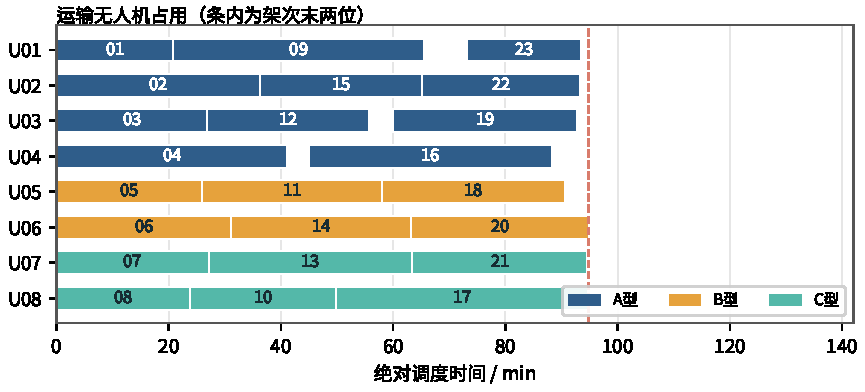
\includegraphics[width=.98\linewidth]{q2_aircraft.pdf}\par\smallskip
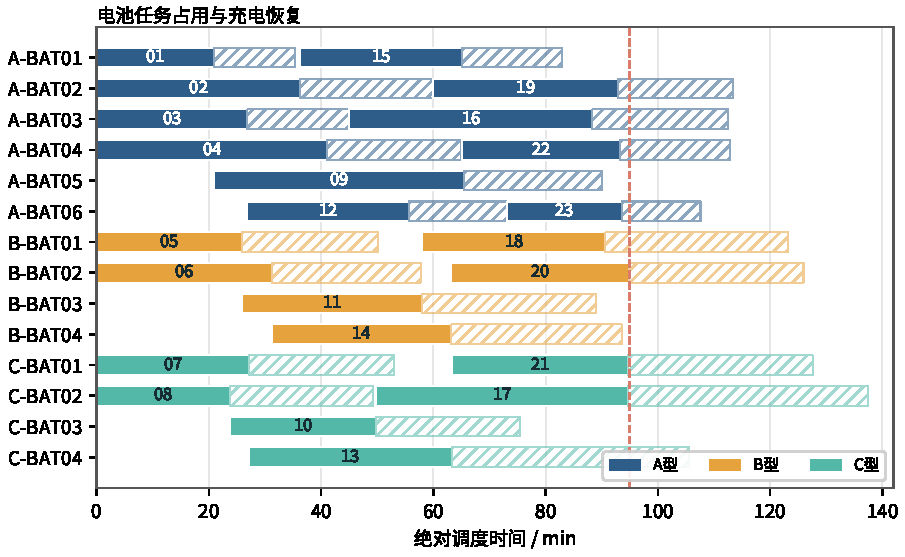
\includegraphics[width=.98\linewidth]{q2_batteries.pdf}
\caption{正式23架次方案的双资源时间表。上图为运输机，下图为电池；浅填充与斜线为充电恢复，虚线为最后返航。所有条块与表\ref{tab:q2_schedule}来自同一份日程。}\label{fig:q2_gantt}
\end{figure}

\subsubsection{箱级时限与返航电量核验}
80箱唯一交付，加权迟到与硬迟到均为0。最后一箱在5283.168387\,s交付，全部运输机在5693.231489\,s返回，相差410.063102\,s，故不能以最后交付替代最后返航。最小硬截止余量202.096058\,s，最低返航SOC为20.097383\%。后者只略高于20\%下限，应理解为名义可行，而非能量误差宽裕。

现有方案曾通过S001两项C型任务的食品箱与卫生用品箱交换，在工期与迟到不变下节省0.011211\,kWh。该调整利用不同载荷组合的能耗差，不改变所有任务的时限可行性。相关箱号以当前正式重放为准。


\subsubsection{机型分工与执行负载}
表\ref{tab:rev_q2_types}按正式日程重新统计运输质量、能耗和工作量。A型11架次承担231 kg，B型6架次承担140 kg，C型6架次承担387 kg。A型以较轻任务提供并行交付能力，C型以较少架次承担较大质量。机型分工由具体任务成本与资源数量共同决定，而非将需求平均拆给八架飞机。

\begin{table}[htbp]\centering\small
\caption{正式运输日程的分机型任务与负载}\label{tab:rev_q2_types}
\begin{tabular}{lrrrrrr}\toprule
机型 & 架次 & 实体数 & 质量/kg & 能耗/kWh & 累计作业/s & 平均负载/s\\\midrule
A & 11 & 4 & 231 & 26.367859 & 21118.826 & 5279.706\\
B & 6 & 2 & 140 & 15.123025 & 11133.183 & 5566.591\\
C & 6 & 2 & 387 & 24.723576 & 11360.487 & 5680.244\\
\bottomrule\end{tabular}
\end{table}


把各类累计作业时间除以实体数量，可得到忽略不可拆任务形态的平均负载下界。C型的该值为5680.243675 s，距正式最后返航仅12.987814 s；B型的平均界为5566.591421 s，其不可拆分配产生更强的离散瓶颈，见下一节。两项统计共同说明，继续改善需要改变接近满负载机型的任务结构，单纯把某一非关键任务提前并不一定改变系统工期。

在共同窗口$[0,T_{\max}]$内，定义飞机$u$的任务占用率及全机群占用率为
\begin{equation}
 U_u=\frac{\sum_{r:a_{ru}=1}p_r}{T_{\max}},\qquad
 U_{\mathrm{fleet}}=\frac{\sum_rp_r}{|\mathcal U|T_{\max}}.
 \label{eq:q2_occupation}
\end{equation}
这里的作业时间包含准备、飞行和交接，因此度量的是任务对实体资源的占用，而非纯空中飞行率。八架飞机的共同窗口占用率为95.76\%。表\ref{tab:rev_q2_util}显示，U06在该窗口上连续作业，两架C型机的占用率均超过99.7\%。这为甘特图中的紧凑安排提供了可复算的量化说明。

\begin{table}[htbp]\centering\small
\caption{共同执行时间窗口内的运输机作业占用}\label{tab:rev_q2_util}
\begin{tabular}{llrrrr}\toprule
实体 & 机型 & 架次 & 作业/min & 非占用/min & 占用率/\%\\\midrule
U01 & A & 3 & 85.808 & 9.080 & 90.43\\
U02 & A & 3 & 93.247 & 1.640 & 98.27\\
U03 & A & 3 & 88.469 & 6.418 & 93.24\\
U04 & A & 2 & 84.457 & 10.430 & 89.01\\
U05 & B & 3 & 90.666 & 4.221 & 95.55\\
U06 & B & 3 & 94.887 & 0.000 & 100.00\\
U07 & C & 3 & 94.620 & 0.268 & 99.72\\
U08 & C & 3 & 94.722 & 0.165 & 99.83\\
\bottomrule\end{tabular}
\end{table}


\subsubsection{交付进度与任务完成层次}
表\ref{tab:rev_q2_milestones}按交接完成事件统计配送进度。30 min完成28箱、268 kg，60 min完成53箱、498 kg，90 min前80箱全部交付。某一早期窗口已交付数量较少，并不表示机群没有工作：首批任务仍可能处于准备、转场或交接阶段，只有完成交接后才能进入交付累计量。

\begin{table}[htbp]\centering\small
\caption{交接完成口径下的累计配送进度}\label{tab:rev_q2_milestones}
\begin{tabular}{lrrrr}\toprule
时刻/min & 已交付箱数 & 质量/kg & 体积/m$^3$ & 箱数进度/\%\\\midrule
15 & 1 & 3 & 0.012 & 1.25\\
30 & 28 & 268 & 0.689 & 35.00\\
45 & 35 & 330 & 0.857 & 43.75\\
60 & 53 & 498 & 1.303 & 66.25\\
75 & 56 & 521 & 1.377 & 70.00\\
90 & 80 & 758 & 2.011 & 100.00\\
\bottomrule\end{tabular}
\end{table}


箱数进度和质量进度反映不同内容。医疗、食品、水和卫生用品的单箱质量不同，故某段时间交付箱数多不必然代表交付质量大。表\ref{tab:rev_delivery_kind}进一步给出各物资类别的交付范围及对应硬时限余量。实际遵守的是每只箱子的原始期限，而不是额外强加“所有医疗箱一定先于所有其他物资”的统一规则。

\begin{table}[htbp]\centering\small
\caption{各物资类别的实际交付时段与硬时限余量}\label{tab:rev_delivery_kind}
\begin{tabular}{lrrrrr}\toprule
物资类型 & 箱数 & 最早交付/min & 最后交付/min & 硬时限箱数 & 最小硬余量/min\\\midrule
医疗物资 & 16 & 14.887 & 86.220 & 16 & 3.368\\
应急食品 & 19 & 15.143 & 88.053 & 0 & --\\
饮用水 & 36 & 15.143 & 88.053 & 15 & 12.889\\
生活卫生用品 & 9 & 21.904 & 86.220 & 0 & --\\
\bottomrule\end{tabular}
\end{table}


从最后一箱交付到全部飞机返航仍有410.063102 s。这段时间属于装备回收，继续占用飞机并产生返航能耗。交付进度和最后返航分别说明物资到位与系统回收两个完成层次，使应急效果和资源周转可以同时核查。

\subsubsection{电池共享的实际接续关系}
23项任务使用14组电池，形成9条再次使用同一电池的接续关系，见表\ref{tab:rev_q2_tight_chains}。其中3条在计算精度内几乎没有充满后的等待。电池池通过不同飞机交替使用已恢复能源支撑多架次，而非一次性分配后永久绑定实体机。

\begin{table}[htbp]\centering\small
\caption{共享电池再次投入任务的接续关系}\label{tab:rev_q2_tight_chains}
\begin{tabular}{lllrrr}\toprule
电池 & 前任务 & 后任务 & 恢复/s & 后项开始/s & 接续余量/s\\\midrule
A-BAT01 & Q2-R-01 & Q2-R-15 & 2121.355 & 2178.800 & 57.445\\
A-BAT02 & Q2-R-02 & Q2-R-19 & 3600.679 & 3600.679 & 0.000\\
A-BAT03 & Q2-R-03 & Q2-R-16 & 2697.242 & 2697.242 & 0.000\\
A-BAT04 & Q2-R-04 & Q2-R-22 & 3895.818 & 3906.224 & 10.406\\
A-BAT06 & Q2-R-12 & Q2-R-23 & 4389.970 & 4389.970 & 0.000\\
B-BAT01 & Q2-R-05 & Q2-R-18 & 3012.098 & 3478.120 & 466.022\\
B-BAT02 & Q2-R-06 & Q2-R-20 & 3463.925 & 3791.400 & 327.475\\
C-BAT01 & Q2-R-07 & Q2-R-21 & 3181.215 & 3799.981 & 618.767\\
C-BAT02 & Q2-R-08 & Q2-R-17 & 2956.347 & 2989.723 & 33.376\\
\bottomrule\end{tabular}
\end{table}


对同电池的相邻任务$r,r'$，定义接续余量
\begin{equation}
 \sigma_{rr'}^B=s_{r'}-(s_r+p_r+c_r).
 \label{eq:q2_battery_slack}
\end{equation}
当恢复时间增加超过该余量，原开始时刻必须调整。接续余量较小的任务是充电压力检验的重点，但局部推迟是否增加最后返航，还取决于另一条资源链何时完成。因此后续实验沿真实依赖传播，不把所有局部延长量直接累加到工期。


\subsubsection{关键资源负载及不同架次数方案比较}
六项B型任务的累计作业时间为11133.182841\,s，分配给两架飞机的平均负载下界为5566.591421\,s。枚举这六个不可拆任务的两机分配，得到更强的离散下界5693.231489\,s，当前日程恰好达到。因而在六项B型箱组、机型、路线固定时，仅换序无法缩短工期；进一步改善须改变任务结构或其他约束，而不是继续调整同一顺序。

原22架次可行见证的工期为7767.058323\,s、能耗66.323024\,kWh；正式23架次方案在两项指标均更小。但该见证不是22架次最优解。本轮短预算稳定性试验还获得6295.573881\,s、71.484859\,kWh的22架次候选，说明22架次方案间也存在较大差异。三者共同支持的是“少一架次不保证更短工期”，而不是“所有22架次方案都必须达到原见证的工期”。


\subsubsection{完成时间下界与可行方案差距}
\label{sec:q2_bound_derivation}
高质量可行解给出上界，但“搜索未改善”不能证明接近全局最优。本文另外采用任务列松弛与互补分支覆盖\cite{barnhart1998branchprice}。下界的关键在于保证每份原问题可行日程都能映射到所求松弛，而不要求松弛解能够反向执行。

\textbf{从实际任务到乐观任务列。}把同一服务区、物资类型、质量及体积的货箱压缩为53个物理类，需求为$d_j$；期限仍留在上界的逐箱验证中，下界不直接施加这些期限。真实航段的时间和能量分别向下取整到毫秒、Wh，再分别作最短路闭包，能量预算向上包络。因此两种闭包不必对应同一条实际航迹，却不会高估实际代价。

在这个删除时限的闭包模型中，可把某服务区全部物资提前到其首次正交付时一起交付，再删除后续重复访问。总装载量、体积和交付数量不变；提前卸货使后续载荷不增，载荷单调能耗与闭包三角不等式保证时间和能耗不增。这个投影论证\textbf{只适用于下界模型}，不能倒过来证明真实山区路线不存在有益的回访。实际定价只要求A、B型不重复访问，C型仍允许回访，因而进一步放松而不排除上述投影。

记乐观列$r$的机型为$g(r)$、交付计数为$a_{jr}$、时间下界为$\underline p_r$（本节统一换算成秒），$n_g$为机型$g$的实体数量。连续主问题为
\begin{equation}
\begin{aligned}
 \min\quad &T\\
 \mathrm{s.t.}\quad&\sum_ra_{jr}x_r=d_j,\quad j=1,\ldots,53,\\
 &\sum_{r:g(r)=g}\underline p_rx_r\le n_gT,\quad g\in\{A,B,C\},\\
 &Bx\le b,\qquad x_r\ge0,\quad T\ge0.
\end{aligned}
\label{eq:q2_relaxed_master}
\end{equation}
根问题的$B$行可为空，节点中则包含有效的整数割和分支条件。任一真实日程的单机累计工作量不超过其最后返航时间，故机型总工作量不超过$n_gT$。这里放松了单架飞机的非抢占接续、共享电池恢复及逐箱时限，故只给下界，不能把分数列解释为配送任务。

\textbf{加强约束与适用条件。}对于货箱类子集$S$，整数覆盖满足
\begin{equation}
 \sum_r\left\lfloor\frac{\sum_{j\in S}a_{jr}}2\right\rfloor x_r
 \le\left\lfloor\frac{\sum_{j\in S}d_j}2\right\rfloor .
 \label{eq:q2_subset_cut}
\end{equation}
其有效性来自整数任务计数和向下取整的次可加性。另在条件$T\le H$下，$H=5465.503$\,s，定义$f_k(p)=\lceil kp/H\rceil-1$。每架飞机上一组任务满足$\sum f_k(p)<(k/H)\sum p\le k$，左侧为整数，所以对$k=2,\ldots,8$有
\begin{equation}
 \sum_{r:g(r)=g}f_k(\underline p_r)x_r\le n_g(k-1).
 \label{eq:q2_packing_cut}
\end{equation}
这些割可排除部分平均工作量合格、却不能装进有限单机时间轴的分数解。它们有$T\le H$的前提，必须把$T>H$的补集一同纳入全局证明。

\textbf{完整定价而不是有限列池的最优值。}对覆盖等式取自由乘子$\pi$，机型工作量和$Bx\le b$分别取非负乘子$\mu,\lambda$。当$\sum_gn_g\mu_g\le1$，且对\emph{所有允许列}有
\begin{equation}
 \bar c_r=\mu_{g(r)}\underline p_r+\lambda^{\mathsf T}B_{\cdot r}
            -\sum_j\pi_ja_{jr}\ge0,
 \label{eq:q2_pricing_rc}
\end{equation}
由弱对偶可得
\begin{equation}
 T\ge\beta=d^{\mathsf T}\pi-b^{\mathsf T}\lambda.
 \label{eq:q2_dual_bound}
\end{equation}
因此，受限列池求得对偶后，还须按机型完整求解$\min_r\bar c_r$。发现负约化成本则加入对应列；没有完成定价时，不把受限主问题目标作为新下界，而保留该区域已有的有效证据。

定价标签保存末节点、质量、体积、能量、时间及相关割状态；A、B型还保存访问集合。两服务区共同配送的分支要求标签保留相应成员状态，只有状态兼容时才能作支配删除，否则可能丢掉负约化成本列。节点中机型$g$对类$j$的总配送量边界为$l_{gj},u_{gj}$时，由覆盖关系再收紧单次停靠的必要上限为$\min\{u_{gj},d_j-\sum_{h\ne g}l_{hj}\}$；这一筛选来自整数可行域，不来自当前列池中是否出现过该组合。

\textbf{互补分支与全域下界。}机型架次数、物理类配送数量、规范化访问次数和两服务区共同配送次数均为整数聚合量。对分数值$v$分成$v\le\lfloor v\rfloor$与$v\ge\lfloor v\rfloor+1$，两子域覆盖该节点的所有规范化真实方案。设完整覆盖的叶域下界为$\beta_\ell$，则包含上述时域补集的全局下界为
\begin{equation}
 LB=\min\left\{H,\min_{\ell\in\mathcal L}\beta_\ell\right\}.
 \label{eq:q2_cover_bound}
\end{equation}
不能取不同叶域下界的最大值，也不能遗漏未解决的子域。不同证明树仅在相同覆盖区域上选择较强的完整子证明；最终仍对整个覆盖取最小值。

正式证据以缩放整数保存乘子，向安全方向修复舍入造成的负约化成本，再对修复后的乘子重新完整定价；分子、分母采用有理数比较。最终下界向下取到微秒，可行上界向上包络。保存的809个分支、810份叶材料和2430次完整机型定价支持
\begin{equation}
 5433.956428\le T^*\le5693.231490\ \mathrm{(s)},\qquad
 \frac{UB-LB}{UB}=4.5541\%.
 \label{eq:q2_bound}
\end{equation}
该确定性区间适用于原始名义实例，不是统计置信区间，也不迁移到改变充电或能耗的新实例。详细叶材料来自已锁定的历史完整认证；本次论文修订核对其数学和数据对应关系，并未重新运行全部2430次定价。附录保留复算入口，正文不以材料数量代替上述有效性链条。



\subsubsection{完整定价怎样把计算结果转为下界}
任务列主问题首先看到的是机型总工作量。两架飞机的工作量除以2给出平均界，但实际任务不能被分成任意小片段，在两条时间轴上的装填可能存在离散不平衡。因此装填割增加了任务长度分布的信息，覆盖约束保证物资数量，分支条件进一步约束整数聚合量，三者共同加强松弛。

另一方面，受限列池可能遗漏便宜任务，直接使用其最优值并不足以形成原问题下界。完整定价检查所有允许列的对偶不等式；Feillet等关于资源约束基本最短路的精确标签算法为此类状态扩展与支配设计提供了方法基础\cite{feillet2004}。本题的定价除了容量和能源，还要保留相关分支状态，使支配删除不会遗漏影响对偶可行性的列。

若全部允许列满足式\eqref{eq:q2_pricing_rc}，则对任一映射到该叶域的实际方案，有
\begin{equation}
\begin{aligned}
 \pi^{\mathsf T}d
 &\le\sum_g\mu_g\sum_{r:g(r)=g}\underline p_rx_r+\lambda^{\mathsf T}Bx\\
 &\le T\sum_gn_g\mu_g+\lambda^{\mathsf T}b
 \le T+\lambda^{\mathsf T}b.
\end{aligned}
\label{eq:q2_weak_dual_chain}
\end{equation}
移项即为$T\ge\pi^{\mathsf T}d-\lambda^{\mathsf T}b$。这个推导说明，完整定价保证的是证书中的对偶可行性，而不只是“列池不再变化”。各叶域分别得到有效界，再通过互补覆盖统一到原问题，才形成最终认证区间。

上界与下界可以沿不同路线持续改善：重构任务和时序降低可行上界，加入有效约束与加强定价提高下界。当前两者相距259.275062 s，量化了名义实例中尚可能存在的工期改进空间。可执行方案与独立界定相结合，使解质量不再仅由一次启发式输出的数值判断。


\subsection{稳健性与敏感性分析}
\label{sec:q2_robust}
\subsubsection{不同随机种子下的结果稳定性}
为避免每次从最终优良方案出发、只重复返回原解而制造“稳定”，先对正式方案进行100次局部扰动提议，保留可行变化，得到一份工期9146.631206\,s的共同可行起点。20个独立随机种子均从该起点出发，各运行150轮搜索，设置120\,s安全上限；全部由轮数限制结束，实测19.919—26.831\,s。每份输出均通过独立物理和完整资源验证。

20次均保持零迟到。工期最小6229.574秒，最大6862.169秒，中位数6457.714秒，样本标准差169.209407\,s，变异系数约2.61\%。架次为22—26，能耗为69.034668—78.336575\,kWh。图\ref{fig:q2_seed}展示全部样本，不只选最好一次。这一结果说明给定起点和短预算能稳定产生可行改进，但均未恢复正式5693.231489\,s水平，不能宣称任意初始解下都稳定得到同等近优解。由于初始即提供可行解，20/20也不是从零构造可行解的成功率。
\fig[.88]{q2_seeds.pdf}{相同起点与150轮预算下20次独立搜索的工期。虚线标出正式方案供参照，但其历史计算预算不同，不用该差值作公平算法排名。}{fig:q2_seed}

\subsubsection{充电时间变化对调度的影响}
将完全充电时间统一乘以$\beta\in\{0.8,0.9,1.0,1.1,1.2,1.3\}$，保留65\%/35\%的两阶段比例。分别检查原始时刻不动的固定日程，以及保持箱组、路线、机型、资源身份和顺序不变、只允许后继开始时刻向后推移的修复日程。对某任务，修复规则为
\begin{equation}
 s_r'=\max\{s_r,t_{\mathrm{aircraft}}',t_{\mathrm{battery}}'\},
\label{eq:q2_repair}
\end{equation}
并按新恢复时间继续传播，不提前任务也不换箱。

充电加快时原日程仍可行，修复规则因不允许提前而不缩短工期。充电时间增加10\%、20\%、30\%时，固定日程分别出现6、6、7处电池接续冲突；顺延修复后均零迟到，工期分别为5802.756723、5955.574471、6108.392219\,s。图\ref{fig:q2_charging}将固定失败与修复代价分开，不能用修复后的成功声称原日程不敏感。
\fig[.88]{q2_charging.pdf}{充电时间倍率与执行代价。叉号表示原固定日程发生资源冲突；曲线为仅顺延开始时刻后的可行结果，不代表重新优化的最短工期。}{fig:q2_charging}

\subsubsection{作业延迟对按时交付的影响}
对23个架次逐一在其第一站交接中增加0、15、30、60、120\,s，每个情景只延迟一个任务，其他交接不变。共115个任务—延迟情景，各检查固定和顺延两种权限，合计230条记录。在当前能耗模型中交接增加时间不另设悬停功率，因而本试验只改变交付、返航和资源时刻，不假称模拟了完整真实悬停能耗。

每个正延迟水平下，固定日程只有9/23个情景保持全部资源与配送条件；其他14个情景首先破坏资源接续，而非出现硬迟到。顺延后23/23均零迟到，所测120\,s单任务延迟的最大工期为5813.231489\,s，比基准增加120\,s。由此可见该方案具有一定时刻修复空间，但原固定日程本身对局部作业延迟敏感。23个确定任务的通过比例不是实际救援成功概率，也不支持多个任务同时延迟的结论。
\fig[.88]{q2_delay.pdf}{单任务首次交接延迟的情景通过数。固定日程与仅顺延修复分开统计；每个延迟水平含23个不同任务情景。}{fig:q2_delay}

\subsubsection{能耗偏差与安全余量的容忍范围}
采用与问题一相同的统一能耗正偏差压力模型，原方案能量边界为
\begin{equation}
 \varepsilon_{\max}=\frac{1-0.2}{1-0.2009738280072748}-1\approx0.121877\%.
\label{eq:q2_energy_limit}
\end{equation}
最低SOC只比下限高0.097383个百分点。本轮在0—2\%范围内对10个能耗水平检查固定与顺延日程，并在边界附近加密。能耗仅增加0.05\%时，原日程已出现3处电池接续冲突；顺延可恢复且不增加最终工期。增加0.13\%后已有一个任务低于20\%SOC，即使调整开始时刻也不能消除能量不可行。这表明“能量容忍范围”与“原时间表容忍范围”仍需分开。

在1\%、2\%压力下进一步开放任务拆分、重新组批、机型与顺序，分别进行250轮搜索。取得的可行备选见表\ref{tab:q2_energy_alternatives}，均由独立扰动物理计算及资源重放核验。它们证明在所测情景下可以通过结构调整恢复，并不证明表中代价最小，也不是原方案已具备同等保障。

\begin{table}[htbp]\centering\small
\caption{能耗偏差下重新调整结构所得可行备选}\label{tab:q2_energy_alternatives}
\begin{tabular}{@{}lrrrcc@{}}
\toprule
偏差 & 架次 & 工期/s & 能耗/kWh & 最低SOC/\% & 独立核验\\
\midrule
1\% & 23 & 5972.072812 & 68.457733 & 20.705 & 通过\\
2\% & 25 & 6650.249809 & 76.308697 & 21.594 & 通过\\
\bottomrule
\end{tabular}
\par\smallskip\parbox{.96\linewidth}{\footnotesize 各250轮搜索；此表为所得可行方案，不宣称情景最优或原方案不变时可用。}
\end{table}


综合而言，名义近优工期与抗扰动能力不是同一个目标。当前日程在小幅时间扰动下可通过顺延恢复，但能量偏差需要更谨慎的结构留量。优先保障稳健执行时，应使用按扰动条件重新验证的备选，而不能仅凭名义最低SOC达标作保证。


\subsubsection{固定资源顺序下的最早顺延修复}
保持箱组、机型、路线、资源身份和顺序不变时，充电或交接时间变化可以沿有向依赖图传播。记任务$r$的原开始为$s_r^0$，同飞机前项为$a(r)$、同电池前项为$b(r)$，扰动后任务与恢复时长为$p'_r,c'_r$，则禁止提前的最早修复满足
\begin{equation}
 s'_r=\max\{s_r^0,\ s'_{a(r)}+p'_{a(r)},\ s'_{b(r)}+p'_{b(r)}+c'_{b(r)}\}.
 \label{eq:q2_maxplus_repair}
\end{equation}
不存在某类前项时省去对应项。原资源顺序来自可行日程，依赖图无环，按拓扑顺序就可完成递推。

该构造在既定顺序和只准向后移动的条件下逐分量最早。初始任务至少要等到原开始和资源可用，取最大值达到下界；若前项已采用最早时刻，任何合法后项都不能早于其释放，所以最大值也给出后项最早开始。沿图归纳即可得到结论。随后再检查箱级截止：如果最早修复已经超期，继续向后移动不能恢复及时性，应改变资源顺序或任务结构。

这使工期变化对应最长依赖路径的增长，而不是扰动总和。两条独立链各推迟30 s可能只延长30 s；同一链上的多个变化则可能累积。单任务延迟实验固定了扰动位置，因此每个恢复结果都可以追溯到具体资源前后关系。

\subsubsection{从压力曲线形成分级调整规则}
充电时间增加30\%时，顺延工期增加415.160730 s，约7.29\%。并行作业吸收了一部分能源恢复延长，只有进入关键接续的部分才传到最后返航。充电加快情景中曲线保持不变，则是因为本次修复不允许提前任务；这与重新优化条件下加快充电可能带来的收益不同。

若仅资源接续被打破而任务仍满足能量安全，优先做时刻修复；若任务自身能耗超过安全预算，改变开始时刻没有作用，应进入重新组批或机型调整。上述两个层次分别对应时间可行性与物理可行性，使压力测试结果可以转为清楚的操作规则。

20次同起点、同预算搜索提供的是解分布，而保存正式方案提供当前最好可行日程，两者在用途上互补。Dolan与Moré提出用明确的性能度量和统一比较对象评估优化软件\cite{dolan2002}。本文相应保留起点、轮数、耗时和全部样本，将短预算稳定性与历史最好解的质量认证分开。研究记录由此既呈现有效改进，也能准确说明计算预算所支持的结论。



\section{问题三：连续通信保障下的运输—中继联合调度}
\label{sec:q3}

\subsection{问题分析与求解思路}
\subsubsection{运输轨迹中的通信需求}
运输任务满足载荷、能量和箱级时限，并不自动保证飞行全过程能与地面网关通信。通信能力随三维位置和地形遮挡变化；中继同时需要满足运输机接入与网关回传，而不是只靠近运输机即可。无人机通信的部署与移动性具有相互影响\cite{zeng2016uavcom,zeng2019sky}，本题将其具体化为每条运输轨迹上的连续链路约束。

\subsubsection{中继位置、服务窗口与运输时刻的耦合}
一处悬停位置是否有效，取决于它能在何时保障哪些航段，以及中继实体和能源组件能否在该时刻到位。提前运输任务可能扩大中继接续压力，移动中继点也会改变转场时间、能耗和通信切换时刻。本文因此先计算候选位置对应的连续可服务区间，再联合选择服务任务与资源顺序，最后精修连续开始时刻。中继与运输均使用真实任务生命周期，不把静态覆盖当作已完成调度。

\subsection{连续通信与联合调度模型}
\subsubsection{直连和单中继链路可用条件}
设端点$a,b$在时刻$t$的三维距离为$d_{ab}(t)$。采用给定自由空间损耗关系\cite{iturp525}和地形附加损耗：
\begin{equation}
 L_{ab}(t)=32.45+20\log_{10}f+20\log_{10}\frac{d_{ab}(t)}{1000}
 +10\,\zeta_{ab}(t),
\label{eq:q3_loss}
\end{equation}
$f=2400$\,MHz，$\zeta_{ab}(t)$表示传播线是否被模型中的地形遮挡。设备功率、天线增益、系统损耗与接收要求共同给出双向允许损耗门限：运输机—网关122\,dB、运输机—中继116\,dB、中继—网关126\,dB。附加传播损耗为$\Delta$时，链路可用条件是
\begin{equation}
 \chi_{ab}(t)=\mathbf1\{L_{ab}(t)+\Delta\le L_{ab}^{\max}\}.
\label{eq:q3_link}
\end{equation}
遮挡计入损耗，而不是一律否决；是否可用仍取决于总损耗与门限。实际网关高度来自输入，不以O01地面位置代替其三维端点。

运输机$U$优先直连网关$G$。直连不可用时，一项在线中继$q$必须同时满足$U\leftrightarrow R_q$和$R_q\leftrightarrow G$。因此
\begin{equation}
 \chi_U(t)=\max\left\{\chi_{UG}(t),\max_{q:\,t\in[a_q,b_q]}
 \chi_{UR_q}(t)\chi_{R_qG}(t)\right\},\qquad \chi_U(t)=1.
\label{eq:q3_provider}
\end{equation}
每时刻只选择一条直连或单中继路径，不构造多级中继网络。提供方的选择需与其真实服务窗口对应；几何可达但尚未上线的中继不能计入式\eqref{eq:q3_provider}。


\subsubsection{链路距离门限与地形状态}
总损耗约束可以在地形状态固定时改写成距离门限。给定遮挡状态$\zeta\in\{0,1\}$和额外损耗$\Delta$，由式\eqref{eq:q3_loss}得
\begin{equation}
 d_{ab}^{max}(\zeta,\Delta)=1000\times10^{\{L_{ab}^{max}-32.45-20\log_{10}f-10\zeta-\Delta\}/20}.
 \label{eq:q3_range_threshold}
\end{equation}
距离单位为m，频率仍用MHz。同一设备下，10 dB遮挡使允许距离变为无遮挡的$10^{-1/2}$，约31.62\%。因而轨迹即使只移动很小距离，只要跨过遮挡事件，也可能改变通信可行性。一个与地形无关的圆形覆盖圈不足以描述这种关系。

固定遮挡状态时，附加0.25 dB使允许距离乘以$10^{-0.25/20}\approx0.9716$，约缩小2.84\%。这个变化可能移动关键服务区间端点，进而影响运输开始时刻。接入与回传又必须同时可用，所以把中继移近运输机改善一跳，并不保证另一跳同步改善。这些关系将空间位置、悬停高度和服务时间联系起来。

\subsubsection{阶段轨迹与通信事件分割}
在一段爬升、巡航或下降中，运输位置可写为$\boldsymbol x(\tau)=\boldsymbol x_0+\boldsymbol v\tau$。对固定通信端点$\boldsymbol p$，距离平方是
\begin{equation}
 d^2(\tau)=\|\boldsymbol v\|^2\tau^2+2\boldsymbol v^{\mathsf T}(\boldsymbol x_0-\boldsymbol p)\tau+\|\boldsymbol x_0-\boldsymbol p\|^2.
 \label{eq:q3_distance_quadratic}
\end{equation}
在遮挡状态不变的区间内，将此式与相应门限平方联立，可以确定进入或离开距离可行域的时刻。交接阶段的位置固定，则退化为常数判定。

地形遮挡部分沿传播线扫过的射线扇面求与闭合像元棱柱的接触事件，再与距离根、阶段端点和服务窗口端点合并排序。相邻事件间没有新状态变化，可用区间内部状态代表该开区间；每个端点另行检查，保留瞬时擦边事件。连续条件因此被转化为有限的区间与端点对象，而不是以稀疏采样近似宣称全过程连通。

\begin{table}[htbp]\centering\small
\caption{连续通信判定中需要保留的事件}\label{tab:comm_events}
\begin{tabularx}{\linewidth}{p{2.8cm}LL}\toprule
事件类型 & 来源 & 对计算的作用\\\midrule
阶段切换 & 爬升、巡航、下降与交接转换 & 更新位置函数和速度\\
地形接触 & 传播线开始或停止触及地形棱柱 & 更新遮挡损耗状态\\
距离门限 & 端点间距达到允许值 & 更新距离可行状态\\
服务窗口端点 & 中继建链完成或停止服务 & 更新在线提供方集合\\
瞬时擦边 & 边、角点和孤立接触 & 对单独时刻核验闭边界条件\\\bottomrule
\end{tabularx}\end{table}

Saunders等对自主配送无人机技术的综述同时讨论航行、通信与任务执行需求\cite{saunders2024}。本题将这些关系集中到可计算的轨迹与服务接口：几何模块说明某链路何时可用，联合排程说明提供方何时真正上线，最终验证检查它们能否覆盖运输执行的全部必要时段。


\subsubsection{中继转场、悬停与能源消耗}
设悬停点$p$的地面高程为$z_g(p)$，悬停海拔为$z_p$，离地高度满足$0<z_p-z_g(p)\le300$\,m。中继转场必须兼容悬停端点，取
\begin{equation}
 H_R(p)=\max\left\{\max_{c\in\mathcal C(O01,p)}Z_c+50,\ z_p,\ h_{O01}\right\}.
\label{eq:q3_relay_height}
\end{equation}
此规则只用于中继，普通运输仍遵守式\eqref{eq:common_cruise_altitude}。对于给定位置分别计算出程与回程时间$t_p^{\mathrm{out}},t_p^{\mathrm{back}}$和转场能耗$E_p^{\mathrm{tr}}$，不能抬高悬停点却保留原转场代价。

中继准备时间为180\,s，建链30\,s，返航周转300\,s；电池可用能量3.2\,kWh，悬停与通信功率合计1.10\,kW。任务$q$的开始为$s_q^R$、实际服务窗口为$[a_q,b_q]$，则
\begin{equation}
 a_q=s_q^R+180+t_{p_q}^{\mathrm{out}}+30,
 \qquad e_q^R=b_q+t_{p_q}^{\mathrm{back}},
\label{eq:q3_lifecycle}
\end{equation}
\begin{equation}
 E_q^R=E_{p_q}^{\mathrm{tr}}+\frac{1.10}{3600}(30+b_q-a_q),
 \qquad E_q^R\le0.8\times3.2.
\label{eq:q3_relay_energy}
\end{equation}
准备时间未额外添加题面未给定的耗电项。中继实体占用延续至$e_q^R+300$，能源组件延续至$e_q^R+\tau(SOC_q)$，两者分别检查，不能将周转、充电和最后返航混为一个时刻。

\subsubsection{连续服务、资源接续与联合完成时间}
对于给定运输任务$i$，把相对开始的直连失效时间集合划成需求区间$h=[\ell_h,u_h]$。记$\mathcal A_h$为能覆盖该整个区间且回传可用的候选中继任务，$z_{hq}$表示选择$q$保障$h$，$y_q$表示启用中继任务。典型覆盖约束为
\begin{equation}
 \sum_{q\in\mathcal A_h}z_{hq}=1,\quad z_{hq}\le y_q,\quad
 z_{hq}=1\Rightarrow
 \begin{cases}a_q\le s_i+\ell_h,\\ b_q\ge s_i+u_h.\end{cases}
\label{eq:q3_cover}
\end{equation}
候选区间的几何条件已确保其内部双跳链路可用；边界接触仍需单独核验。中继实体与能源组件均须唯一指派，同一实体的占用不能重叠；运输侧继续满足箱级时限、20\%返航余量及飞机—电池约束。在零迟到条件下最小化
\begin{equation}
 T_{\max}^{\mathrm{joint}}=\max\left\{\max_i(s_i+p_i),\max_q e_q^R\right\}.
\label{eq:q3_objective}
\end{equation}
最后返航后的充电和中继周转参与资源接续，但不额外延长式\eqref{eq:q3_objective}。时间优先、节能及增强通信保障分别保留方案，不将dB、kWh和秒任意加权为一个分数。


\subsubsection{服务窗口与两类中继资源的连接}
几何覆盖和时间覆盖分别承担不同约束。候选位置属于$\mathcal A_h$，表示能够满足需求区间$h$的接入和回传；实际指派$z_{hq}=1$后，还要求其在线窗口包含运输的绝对需求区间。几何条件成立而中继未到位时，不能向运输任务提供服务。

中继任务同时占用实体机和能源组件。若$q'$使用执行$q$的同一架中继机，需要等到$q$返航并完成周转；若使用同一能源组件，则需要等到该组件充满。两种接续分别为
\begin{equation}
 s_{q'}^R\ge e_q^R+t^{turn},\qquad
 s_{q'}^R\ge e_q^R+c_q^R,
 \label{eq:q3_two_relay_resources}
\end{equation}
各式仅在对应资源相同且$q$为前项时启用。题目允许同型资源复用，因此同一中继机可更换组件，已恢复组件也可供另一实体机使用。

服务结束$b_q$同时决定返航时刻、悬停能耗和能源恢复。延长窗口可能覆盖更多运输需求，却推迟后续资源；删去不必要的早到悬停，则可能同时节能并改善接续。将服务起止保留为连续变量，才能把通信保障真正纳入调度，而不是在运输时间表外另放若干静态点。

\subsubsection{分层计算中的决策接口}
候选重定位负责新的位置、高度和传播关系，联合整数模型负责任务选择、提供方和资源路径，固定结构线性规划负责最后的连续时刻。空间计算不直接塞进整数规划的代数约束，而是生成可审查的可服务关系；给定离散选择后，时间条件尽量交给线性优化精确处理。

这种接口还说明了扰动后的处理层次：只改变中继最早上线时刻，可复用几何并修复时序；传播门限改变，需要重检距离根与可服务区间；候选不再能覆盖关键需求，则回到提供方或位置选择层。每次调整都以同一运输需求和物理规则为基础，避免不同模块分别“优化”后得到互不兼容的日程。



\subsection{中继部署与任务时序的联合求解}
\subsubsection{候选悬停位置生成与可服务区间计算}
本节区分题目要求的联合决策空间与实际搜索的有限子域。求解从已保存的23项运输任务和4个中继位置起步，对位置、高度、资源顺序和通信切换进行局部改进；另以小规模运输任务重组检验是否能进一步改善。候选的初始箱组、路线及部分悬停位置继承自补充资料，具体来源与本项目新增计算分列于附录\ref{app:source_provenance}，不把所有初始结构描述为从零构造。

\begin{table}[htbp]\centering\small
\caption{联合求解各阶段的开放变量与固定范围}\label{tab:q3_decision_scope}
\begin{tabularx}{\linewidth}{p{2.4cm}XX}\toprule
阶段 & 允许改变的对象 & 固定内容与输出\\\midrule
位置候选搜索 & 单个中继的水平位置和离地高度 & 暂固定运输模式与其他中继；输出少量候选，尚不宣称完整可行\\
运输重组对照 & 小货箱并集中的组批、机型、访问顺序及选中任务数 & 只在显式给定的有限任务池内选择；未截断的枚举与截断池分开记录\\
联合整数排程 & 候选任务选择、开始时刻、提供方、飞机/电池及中继实体顺序 & 单个任务的路线、单个中继槽的位置已给定；输出可行离散结构\\
连续时间精修 & 运输开始、中继服务开始/结束及联合工期 & 固定路线、位置、提供方、真实资源顺序与充电分段；输出时刻\\
独立验收 & 不再改变计划 & 从完整几何重建区间、端点、能量与资源占用，接受或拒绝候选\\\bottomrule
\end{tabularx}
\end{table}

位置生成在当前点附近按水平网格偏移，并枚举25、50、\ldots、300\,m共12个离地高度。默认搜索半径1200\,m、网格300\,m、每个角色保留10个候选；保存的局部试验还使用75\,m和50\,m尺度，以及面向关键角色的扩大探测，均为有限试验域。先检查DEM覆盖、AGL、回传链路和中继转场，再以任务阶段严格内部、约25\,s间隔的采样估计接入潜力。评分按角色优先考虑出程、回程或二者之和，并以链路裕度破同分；保留水平位置互异的短名单。这里的抽样只可能筛选候选，不能作为整个连续空间不可行的证据。

每个保留点都重新建立完整几何。运输机在一个飞行阶段内位置随时间线性变化；固定端点至该阶段的射线扇面与DEM地形棱柱求交，得到遮挡事件区间，再加入距离门限的解析交点、飞行阶段和服务窗口边界。相邻端点之间的开区间内状态固定，检查内部状态并单独检查全部临界端点，保留孤立擦边事件。这一步才产生式\eqref{eq:q3_cover}使用的可服务关系，不用采样连线替代。

候选搜索先比较完整求解后的工期，再比较同工期能耗；当前实现的接受阈值为工期改善超过0.005\,s，或工期差不超过0.005\,s时能耗改善超过0.005\,kWh。该阈值仅用于有限搜索的数值筛选，不代表实际执行的抗扰动余量。一次角色扫描或预定网格完成后停止，不能宣称无导数全空间搜索已经收敛。

\subsubsection{通信提供方与资源顺序的联合选择}
对有限运输任务池$\mathcal I$取选择变量$x_i$，逐箱覆盖沿用式\eqref{eq:q2_cover}；只重排已有23项任务时固定$x_i=1$。每个中继槽$q$对应一个候选位置，取启用变量$y_q$及式\eqref{eq:q3_cover}的提供方变量$z_{hq}$。需求属于任务$i$时，将覆盖等式右端写为$x_i$，未选择任务不再产生通信需求；$z_{hq}\le y_q$，同时禁止启用不服务任何需求的中继槽。

有限模型通过\emph{任务可接续路径}控制资源数量。对同型飞机，二元变量$v^U_{ij}$表示任务$j$紧接$i$，$o_i^U$表示任务$i$占用一条资源链的起点，满足
\begin{equation}
\begin{aligned}
 o_i^U+\sum_jv^U_{ji}&=x_i,&\sum_jv^U_{ij}&\le x_i,\\
 \sum_{i:m_i=m}o_i^U&\le n_m^U,&
 v^U_{ij}=1&\Rightarrow s_j\ge s_i+p_i .
\end{aligned}
\label{eq:q3_transport_paths}
\end{equation}
电池路径将$p_i$替换为$p_i+c_i$，起点数上限替换为该型号电池库存。正时长的先后约束排除环，故每条路径可以赋予一个实体资源编号。中继实体同样构造路径，接续条件为后项任务开始不早于前项返航加300\,s周转。条件式以二元变量和由有限时间上界计算的大常数实现，不用一个无根据的无限大数。

选定位置后，中继服务开始$a_q$、结束$b_q$以及任务开始$\sigma_q$满足式\eqref{eq:q3_lifecycle}的启用形式：$\sigma_q=a_q-\ell_qy_q$，$\ell_q=180+t^{out}_{p_q}+30$；$b_q\ge a_q$，能耗为转场项、建链项及服务时长项之和。服务覆盖用$z_{hq}$连接运输和中继时间轴。运输硬截止在该阶段另保留30\,s的算法性余量，期望送达仍要求零迟到；30\,s不是新添题设，而是本次搜索采用的保守限制。

当前中继架次试验最多启用6个槽，初始满电能源组件为6组，因此内层整数模型可先让每个启用中继任务使用不同组件，保证存在不复用的组件指派，不需要在此阶段对组件再建组合接续变量。选出任务后，按真实含充电区间重新构造组件复用链，正式方案只需3组；后续连续精修显式保留这3组组件的恢复关系。这一简化依赖“启用任务数不超过初始组件数”，不能直接推广到更多中继架次。

先用HiGHS求有限模型的最小联合工期，再在已得工期增加不超过$10^{-5}$\,s的条件下，允许整数关系继续改变并最小化总能耗。接着固定实际资源链进入下一节的连续精修。当前保存的设置为单线程、整数相对间隙$10^{-7}$、整数可行性容差$10^{-7}$；公开重复优化入口默认90\,s预算，历史各局部试验的实际限时分别保存在状态文件中，不把入口默认值当作所有试验的实际耗时。

\textbf{运输结构和架次数的作用。}除固定23项任务外，程序也对小货箱并集重新生成模式：并集不超过11箱时枚举非空子集、可用机型及路线；模式超过250项时按单位箱数时间、单位箱数能耗和最迟启动余量交错截断。保存对照覆盖S006/S007、S004/S005、S003/S015等组合，联合任务池最大361项，未得到比对应参考更好的已验证运输结构。因此本章主方案与同模型改进前方案的23项箱组、机型和有序路线逐项相同，约87.998\,s的成功改进应归于中继位置与联合时序，而不是运输重组。

\begin{table}[htbp]\centering\small
\caption{不同运输及中继架次试验的实际范围}\label{tab:q3_sortie_scope}
\begin{tabularx}{\linewidth}{p{3.0cm}XX}\toprule
对照 & 搜索范围与结果 & 可作出的结论\\\midrule
运输模式重组 & 小并集与有限路线池，最高361个候选；部分试验限时，未选出更好的正式结构 & 运输架次数可在池内改变；主方案23架次是最终选中结果，不是全局最少证明\\
3个中继架次 & 给定所测4个位置和完成时间上限，有限模型不可行 & 只排除该布局及时间阈值下的三架次方案\\
最多5或6架次 & 8个同位置重复出动槽；普通模型限时未改善 & 未改善或超时不证明所有增加架次的方案无效\\
最多5架次加对称消除 & 同位置槽安全重标号后，有限模型最优仍选4项 & 该有限模型无需第5项；不构成连续位置空间的四架次下界\\\bottomrule
\end{tabularx}
\end{table}

阶段性保存工期依次出现5924.967、5895.017、5866.141、5857.090和5836.970\,s。位置、资源顺序和能耗再优化在不同阶段同时调整，所以该轨迹是实际搜索进展，不是逐因素可加的消融分解。全部保存状态包括110份整数模型结果（91份有限域最优、15份有限域不可行、4份限时）及125份连续精修记录；记录数不能等同于不同有效方案数。

\subsubsection{给定任务结构后的时间安排优化}
\label{sec:q3_fixed_lp}
为使时刻精修可直接复核，本节给出实际使用的固定结构线性模型。输入固定运输箱组、机型、路线，中继位置，通信区间的提供方，以及飞机、电池、中继实体和组件的前后顺序。变量为运输开始$s_i$、中继服务开始$a_q$、服务结束$b_q$和联合最后返航$M$。记$\ell_q=180+t_{p_q}^{out}+30$，则任务开始$\sigma_q=a_q-\ell_q$、返航$e_q=b_q+t_{p_q}^{back}$。

对运输任务，根据箱级要求计算
\begin{equation}
 \bar s_i=\min\left\{\min_{b\in\mathcal B_i}(d_b-\delta_{ib}),\;
 \min_{b\in\mathcal B_i\cap\mathcal B_H}(h_b-\delta_{ib}-30)\right\},
 \quad 0\le s_i\le\bar s_i .
 \label{eq:q3_lp_start_bounds}
\end{equation}
$\mathcal B_H$是存在硬截止的货箱集合，空集最小值取正无穷。已固定给中继$q$的相对需求区间$[\ell_h,u_h]$满足
\begin{equation}
 a_q\le s_i+\ell_h-g_s,\qquad b_q\ge s_i+u_h+g_s,
 \quad a_q\ge\ell_q,\quad b_q\ge a_q .
 \label{eq:q3_lp_coverage}
\end{equation}
实际$g_s=10^{-4}$\,s是数值保护间隔。提供方在进入此模型前按完整可服务关系确定，线性规划本身不再自由改派或移动中继。

固定位置的转场能耗为$E_q^{tr}$，令$w=1.10/3600$\,kWh/s，则
\begin{equation}
 E_q=E_q^{tr}+w(30+b_q-a_q),\qquad 0\le E_q\le0.8B_R,
 \quad B_R=3.2\ \mathrm{kWh}.
 \label{eq:q3_lp_energy}
\end{equation}
充电按名义任务所在的分段固定，并同时施加保持该分段的能量条件，不能只线性化而遗漏分段边界。若$E_q\le0.1B_R$，则$c_q=(3.5\tau_R^{full}/B_R)E_q$；若$E_q\ge0.1B_R$，则
\begin{equation}
 c_q=\frac{0.65\tau_R^{full}}{0.9B_R}E_q
       +\tau_R^{full}\left(0.35-\frac{0.65\times0.1}{0.9}\right).
 \label{eq:q3_lp_charge}
\end{equation}
两段在$E_q=0.1B_R$处连续。该表达由式\eqref{eq:common_recharge}代入$SOC=1-E_q/B_R$得到。

对固定资源链上的相邻任务，分别要求
\begin{equation}
\begin{aligned}
 s_j&\ge s_i+p_i+g_r &&\text{（同一运输机）},\\
 s_j&\ge s_i+p_i+c_i+g_r &&\text{（同一运输电池）},\\
 a_v-\ell_v&\ge b_q+t_{p_q}^{back}+300+g_r &&\text{（同一中继机）},\\
 a_v-\ell_v&\ge b_q+t_{p_q}^{back}+c_q+g_r &&\text{（同一中继组件）}.
\end{aligned}
\label{eq:q3_lp_resource}
\end{equation}
其中$g_r=10^{-4}$\,s，运输$c_i$因任务属性固定而为常数；中继$c_q$由式\eqref{eq:q3_lp_energy}--\eqref{eq:q3_lp_charge}给出仿射函数。目标为
\begin{equation}
 \min M,\qquad s_i+p_i\le M,\quad b_q+t_{p_q}^{back}\le M .
 \label{eq:q3_lp_objective}
\end{equation}
还保留实现中的20000\,s变量上界；当前解远未触及该数值边界。求出$M_{LP}^*$后，再加$M\le M_{LP}^*+10^{-6}$\,s并最小化$\sum_q E_q$。两轮均使用SciPy HiGHS，原始及对偶可行性容差为$10^{-8}$。

该线性规划的工期下界为5836.969928328251\,s，二次节能后的保存值比其大$10^{-6}$\,s。因此可称给定路线、位置、提供方、资源顺序和充电分段的连续时序已闭合；不能称原问题全局最优，也不能把数值保护间隔或求解精度当作实飞时序容错。最终计划仍返回未修改的完整物理与连续通信验证器验收。



\subsubsection{给定结构的连续精修与复核接口}
运输路线和载荷固定后，运输作业与充电时长为常数；中继位置固定后，转场时间为常数，服务时长决定线性悬停能耗。再固定各组件处于哪一充电分段，并保留该段能量上下界，资源接续就具有仿射形式。这些条件共同解释固定结构模型为什么可以采用线性规划。

分段边界是模型的一部分。只使用一段充电直线而不约束能量范围，可能算出原函数不支持的恢复时刻。两轮优化先压缩联合工期，再在给定工期容许量内减少不必要的服务能耗，所得解仍须返回完整物理计算和通信事件核验。Huangfu与Hall给出的对偶修正单纯形研究为所用线性规划技术提供方法背景\cite{huangfu2018}；本文的固定结构结论则来自明确的输入、约束及保存下界。

位置和任务组合选择、资源先后安排、具体开始时刻分属不同规模的决策。分层方法使每一层都有可列出的输入与输出，也使恢复计算能只调整受扰动的层次。数值保护间隔用于提高计算稳定性，执行保障范围则由本章实际压力情景和连续核验单独评价。


\subsection{联合方案与结果验证}
\subsubsection{运输日程与中继部署方案}
工期优先方案由23个运输架次和4个中继架次组成，使用8架运输机、14组运输电池、2架中继机、3组中继能源组件。联合最后返航5836.969929\,s，总能耗68.939416\,kWh，其中运输66.251280\,kWh、中继2.688136\,kWh。80箱唯一交付，零加权迟到、零硬迟到，最小硬截止余量360.866938\,s。

全部23项运输任务的飞机、电池、开始、末箱交付与返航时刻见附录表\ref{tab:q3_full_schedule}，不沿用问题二的时刻；表\ref{tab:q3_sites}和表\ref{tab:q3_relays}给出四项中继任务的实际部署与服务时刻；编号“中继任务”与“实体中继机”严格区分。第一架实体先执行Q3-R-02，再执行Q3-R-01；第二架先执行Q3-R-03，再执行Q3-R-04。四个架次不是四架实体机。

\begin{table}[htbp]\centering\small
\caption{中继任务、实体资源与悬停位置}\label{tab:q3_sites}
\begin{tabular}{@{}lllrrr@{}}
\toprule
中继任务 & 实体 & 能源组件 & 经度 & 纬度 & AGL/m\\
\midrule
Q3-R-01 & R01 & R-ENG02 & 109.201003 & 23.033703 & 300\\
Q3-R-02 & R01 & R-ENG01 & 109.268309 & 23.014741 & 275\\
Q3-R-03 & R02 & R-ENG02 & 109.211343 & 23.020248 & 300\\
Q3-R-04 & R02 & R-ENG03 & 109.237677 & 23.059303 & 300\\
\bottomrule
\end{tabular}
\end{table}


\begin{table}[htbp]\centering\small
\caption{四项中继任务的实际服务时间表}\label{tab:q3_relays}
\begin{tabular}{@{}lrrrrr@{}}
\toprule
任务 & 开始/min & 服务开始 & 服务结束 & 返航/min & SOC/\%\\
\midrule
Q3-R-01 & 59.312 & 69.709 & 89.566 & 97.228 & 81.294\\
Q3-R-02 & 2.661 & 12.595 & 47.178 & 54.312 & 73.307\\
Q3-R-03 & 5.531 & 13.606 & 24.386 & 29.603 & 89.079\\
Q3-R-04 & 34.603 & 46.546 & 78.701 & 87.860 & 72.316\\
\bottomrule
\end{tabular}
\end{table}

\fig[.89]{q3_deployment.pdf}{工期优先方案的中继悬停位置与关键运输路线。中继点为实际位置，不用圆形覆盖圈代替地形条件下的可服务区域。}{fig:q3_deployment}
\fig[.97]{q3_resources.pdf}{四项中继任务的实体复用与服务窗口。深色表示实际服务；任务开始、服务开始、返航和周转分别处理。}{fig:q3_resources}

\subsubsection{连续通信及资源占用核验}
本轮从完整运行包重新构造名义几何和计划，八项核心导出与保存结果逐字节一致。独立验证完成17756项物理、能源、资源、完整区间和端点检查，失败0；另有36672个包含边界的时空核验点，失败0。保存的700份区间材料与1238份临界端点材料用于追溯覆盖，不能把核验计数当作实飞次数或随机稳定性样本量。

最低运输返航SOC为20.097383\%，最低中继SOC为72.315816\%。中继能源较宽裕不意味着通信时间宽裕。图\ref{fig:q3_provider}以关键任务的实际通信提供方显示切换关系，服务端点必须与中继在线窗口相互兼容。若只画静态连接网络，将无法发现这种时间瓶颈。
\fig[.93]{q3_providers.pdf}{关键运输任务的阶段与实际通信提供方。横轴为绝对调度时间，提供方切换来自正式区间记录，不是抽样插值。}{fig:q3_provider}


\subsubsection{运输与中继能源成本的分解}
联合方案运输能耗66.251280 kWh，中继能耗2.688136 kWh，中继占总能耗约3.90\%。表\ref{tab:rev_q3_transport_energy}按51条实际运输航段聚合，水平部分63.050347 kWh，爬升部分3.200933 kWh。爬升项在总量中所占比例较小，但仍会改变接近安全边界任务的机型和箱组可行性，因此在逐段计算中完整保留。

\begin{table}[htbp]\centering\small
\caption{联合方案运输能耗的物理分解}\label{tab:rev_q3_transport_energy}
\begin{tabular}{lrrr}\toprule
机型 & 水平能耗/kWh & 爬升能耗/kWh & 总能耗/kWh\\\midrule
A & 24.888150 & 1.516529 & 26.404679\\
B & 14.308489 & 0.814536 & 15.123025\\
C & 23.853709 & 0.869867 & 24.723576\\
\bottomrule\end{tabular}
\end{table}


四项中继任务的转场合计0.866261 kWh，建链和实际服务合计1.821876 kWh，后者约占中继能耗的67.77\%。表\ref{tab:rev_q3_relay_energy}显示，各任务服务10.780—34.583 min，占自身准备至返航作业时间的44.78\%—66.96\%。中继成本不仅取决于飞到哪里，还取决于在那里等待和服务多久。

\begin{table}[htbp]\centering\small
\caption{中继任务的转场、建链与悬停服务成本}\label{tab:rev_q3_relay_energy}
\begin{tabular}{lrrrrr}\toprule
中继任务 & 转场/kWh & 建链及服务/kWh & 总能耗/kWh & 服务/min & 服务占用比/\%\\\midrule
Q3-R-01 & 0.225372 & 0.373222 & 0.598594 & 19.858 & 52.37\\
Q3-R-02 & 0.210978 & 0.643196 & 0.854174 & 34.583 & 66.96\\
Q3-R-03 & 0.142681 & 0.206793 & 0.349474 & 10.780 & 44.78\\
Q3-R-04 & 0.287229 & 0.598665 & 0.885894 & 32.154 & 60.38\\
\bottomrule\end{tabular}
\end{table}


能源充足和服务及时是两种条件。中继返航SOC较高，提供了能源上的余量；但如果它未在关键切换前完成建链，运输任务仍可能等待。因而改善一个方案应先识别起作用的约束：位置可能主要改善遮挡和交接，开始时刻可能主要减少提前悬停，组件配置则主要影响跨架次恢复。这些作用都能在分解表与实际服务窗口中对应。

\subsubsection{通信提供方的实际保障工作量}
从正式保存的181个通信阶段、228条实际提供方区间重新聚合，运输任务累计需要34312.495780 s保障。固定网关承担20734.854799 s，占60.43\%；中继承担13577.640980 s，占39.57\%。18个运输架次在部分阶段使用中继，5个全程直连，见表\ref{tab:rev_q3_provider}。

\begin{table}[htbp]\centering\small
\caption{实际通信提供方的累计保障工作量}\label{tab:rev_q3_provider}
\begin{tabular}{lrrrr}\toprule
提供方 & 区间数 & 运输任务数 & 累计保障/min & 比例/\%\\\midrule
G01 & 112 & 23 & 345.581 & 60.43\\
Q3-R-01 & 41 & 7 & 92.738 & 16.22\\
Q3-R-02 & 28 & 7 & 48.093 & 8.41\\
Q3-R-03 & 15 & 3 & 24.757 & 4.33\\
Q3-R-04 & 32 & 9 & 60.706 & 10.62\\
\bottomrule\end{tabular}
\end{table}


累计保障时长按运输任务分别求和。如果两架运输机在同一秒使用同一中继，该秒贡献两份保障工作量。因此Q3-R-01约19.858 min的在线窗口，可对应约92.738 min的多任务累计保障。该指标说明其承担的任务服务量，不是系统失联时长、通信吞吐量或中继自己的飞行时长。当前模型没有额外的并发用户容量约束，保障关系按给定双跳链路条件核算。

实际提供方序列在合并相邻同提供方记录后共有47次切换，包括直连—中继和中继—中继交接。表\ref{tab:rev_q3_comm_tasks}列出中继保障需求较大的任务。相对于静态“覆盖多少服务区”，这些记录更直接回答：中继为哪些运输机服务、在什么时段服务、哪些切换会影响任务开始。

\begin{table}[htbp]\centering\small
\caption{中继保障需求较大的运输任务}\label{tab:rev_q3_comm_tasks}
\begin{tabular}{lrrr}\toprule
运输任务 & 直连/min & 中继/min & 提供方切换数\\\midrule
Q3-T-09 & 13.587 & 24.505 & 3\\
Q3-T-16 & 14.928 & 21.465 & 3\\
Q3-T-17 & 16.300 & 20.589 & 3\\
Q3-T-12 & 11.503 & 16.227 & 3\\
Q3-T-20 & 12.676 & 13.521 & 2\\
Q3-T-10 & 12.263 & 13.283 & 3\\
Q3-T-21 & 12.676 & 13.021 & 2\\
Q3-T-15 & 21.829 & 12.739 & 4\\
\bottomrule\end{tabular}
\end{table}


中继以较小的能源占比支撑较大比例的运输通信任务时间，体现了运输与通信资源的分工价值。该统计不替代优化证明，而为联合方案增加运行机理说明：空间部署提供可用链路，服务窗口保证时间匹配，实体和组件复用保证这些服务能够实际安排。


\subsubsection{通信切换对最后返航时间的影响}
与采用同一悬停兼容物理模型的改进前方案相比，当前方案工期缩短87.997560\,s。关键C型任务前段保障结束的相对时刻由956.973974延长至1039.150288\,s，即交接边界后移82.176314\,s；后继中继又提前5.821245\,s就绪，二者共同放松其最早开始约束。这些差值是同物理模型的保存对照，不能与更早的受限高度模型混合归因。

当切换约束活跃时，其形式可写为$s_i\ge a_q-\ell_h+g$，其中$g$是计算保护间隔。后继可服务时刻$a_q$提前、前段可持续时长$\ell_h$增加，都会使运输任务更早开始。当前末尾的S007—S003 C型任务与S011 A型任务同在5836.969929\,s返航；最后中继在5833.697980\,s返回。由此，优化中继的价值体现在减少运输等待，而不只是减少中继自己的飞行距离。

\subsubsection{工期优先与节能备选方案比较}
节能备选在5911.548秒完成，能耗为68.735791 kWh；比工期优先方案晚74.578秒、节省0.203625\,kWh。面向三组独立配置的折中方案为5866.140527\,s、68.975497\,kWh；它在时间与能耗上并不优于工期优先方案，但后续三组资源缺口较小，见第\ref{sec:q4}章。上述都是已验证的离散候选，不代表完整Pareto前沿或全局最优解。

\subsection{稳健性与敏感性分析}
\label{sec:q3_robust}
\subsubsection{附加传播损耗下的通信可行性}
分别固定工期优先方案与附加0.25\,dB保障备选的路线、位置、运输时刻和原中继提供方，在$\Delta=0,0.05,0.10,0.15,0.20,0.25$\,dB下重做完整区间与端点核验。允许遵守直连优先规则使用可用直连，但不切换到另一项未指派中继，也不移动日程。新增损耗门限解析交点与全部几何擦边端点一同检查，不能用原来的少量采样点判断新阈值。

表\ref{tab:q3_loss}表明：工期优先方案在名义条件通过，附加0.05\,dB即失去连续通信，按不同运输任务分别累计的失联时长为138.973270\,s；0.25\,dB时为503.429111\,s。该总量是各任务失联时长之和，不是整个系统墙钟时间的并集，也不是丢包量。增强保障备选在全部六个水平的区间和端点检查均通过。固定物理与提供方时，门限条件对$\Delta$单调，故通过0.25\,dB也支持该模型下整个$[0,0.25]$区间，不支持更大的未测损耗。

\begin{table}[htbp]\centering\small
\caption{附加损耗下两份固定方案的连续通信核验}\label{tab:q3_loss}
\begin{tabular}{@{}rrcrc@{}}
\toprule
损耗/dB & 原方案失联/s & 核验 & 增强方案失联/s & 核验\\
\midrule
0.00 & 0.000 & 通过 & 0.000 & 通过\\
0.05 & 138.973 & 失效 & 0.000 & 通过\\
0.10 & 300.470 & 失效 & 0.000 & 通过\\
0.15 & 368.384 & 失效 & 0.000 & 通过\\
0.20 & 436.035 & 失效 & 0.000 & 通过\\
0.25 & 503.429 & 失效 & 0.000 & 通过\\
\bottomrule
\end{tabular}
\end{table}

\fig[.88]{q3_loss.pdf}{固定两份方案后的附加损耗响应。纵轴为逐运输任务累计失联时长；增强保障备选与原工期优先方案分别核验，不混合统计。}{fig:q3_loss}

0.05\,dB是首个已测失效水平，不是精确最大容忍损耗。这里“失去通信”指当前模型和原提供方约定下的结果，不是实测链路失效概率。旧候选域的0.50/0.55\,dB结论不进入本试验。更重要的是，增强方案的成功不能被写成原工期优先方案本身能够承受0.25\,dB。

\subsubsection{中继到位延迟下的服务连续性}
对四项中继任务分别将最早可服务时刻向后移0、1、5、10、30、60\,s，运输时刻、原中继提供方及原定服务结束保持不变，形成24个情景。这模拟部署端迟发或上线延后造成的可用性丧失；转场路径与速度不变，不把它解释为飞行变慢或额外空中等待，因此不虚构额外飞行功率。

四项任务在所测1\,s延迟下均失效，但这不是精确临界延迟。以30\,s为例，Q3-R-01至Q3-R-04分别造成60.000、30.000、70.557、89.984\,s逐任务累计失联，说明被保障运输任务数和切换边界决定传播影响，不是延迟秒数的简单一比一映射。

随后对每项中继的5、30、60\,s延迟开放时序修复：路线、悬停位置、资源身份与顺序、通信覆盖指派和充电分段保持不变，只允许运输开始和中继服务边界向后调整，不提前任务。连续线性模型先最小化联合返航，再在该工期上尽量节省悬停能耗；12份输出全部回到完整物理模型重算，并经过区间、端点与独立时空点检查，零失败、零迟到。

\begin{table}[htbp]\centering\small
\caption{固定结构修复中继上线延迟的额外工期}\label{tab:q3_repair}
\begin{tabular}{@{}lrrrc@{}}
\toprule
延迟任务 & 延迟5秒 & 延迟30秒 & 延迟60秒 & 完整核验\\
\midrule
Q3-R-01 & 5.000 & 30.000 & 60.000 & 3/3通过\\
Q3-R-02 & 5.000 & 30.000 & 60.000 & 3/3通过\\
Q3-R-03 & 1.403 & 26.403 & 56.403 & 3/3通过\\
Q3-R-04 & 1.728 & 26.728 & 56.728 & 3/3通过\\
\bottomrule
\end{tabular}
\par\smallskip\parbox{.96\linewidth}{\footnotesize 中间三列均为新增工期/s，不是修复后总工期；转场物理参数保持不变。}
\end{table}

\fig[.89]{q3_repair.pdf}{给定任务结构下修复中继上线延迟的工期代价。每个点均经完整模型核验；曲线只连接已计算情景，不表示全局最优恢复策略。}{fig:q3_repair}

30\,s延迟的新增工期为26.403—30.000\,s，60\,s延迟为56.403—60.000\,s。部分修复后的中继能耗略减，因为延后部署缩短了无必要的提前悬停，并非飞行延迟可以“免费节能”。若实际情景包含额外空中等待，需要另设相应时间和功率再核验。上述结果支持存在时序恢复能力，但不能把恢复后的成功归为固定原方案稳健。

\subsubsection{保障裕度与工期、能耗的权衡}
附加0.25\,dB保障备选的联合工期5866.140527\,s，总能耗69.031751\,kWh，相比工期优先方案增加29.170597\,s和0.092335\,kWh。这是两份具体方案间的保障代价，不是所有增强保障方案的最小必要代价。针对上线延迟的12次修复也只在给定结构内优化，不扩张为自由位置、路径、分组同时可调的全局结果。

因此本问的稳健性结论是有条件的：名义最快候选在小幅传播损耗或1\,s上线延迟下已可能失效；增强损耗备选和明确的时序修复提供了可验证的补救。选择方案时应区分所需保障类型，不能用中继较高剩余电量或求解器微小间隙替代通信时间裕度。


\subsubsection{通信交接约束的恢复解释}
对关键运输任务$i$，若前段提供方可持续至相对时刻$\tau_i^{sw}$，后继中继$q$在绝对时刻$a_q$可用，含保护间隔$g$的交接要求可写为
\begin{equation}
 s_i+\tau_i^{sw}\ge a_q+g
 \quad\Longleftrightarrow\quad
 s_i\ge a_q-\tau_i^{sw}+g.
 \label{eq:q3_handoff_start}
\end{equation}
后继中继提前和前段保障延长，均可降低通信给任务开始施加的下界。当前同模型改进把这两方面结合，解释了约87.998 s工期下降。改进后两项运输末任务同刻返回，也说明下一轮位置调整可能遭遇新的资源瓶颈，收益不会无限线性叠加。

名义工期优先、增强通信保障和扰动后修复构成三类执行选择。附加0.25 dB保障备选比主方案增加约0.50\%工期、0.13\%能源；单项上线延迟则优先保持位置与路线、重新安排服务和运输时刻。12份修复给出了所测5、30、60 s上线延迟下的实际恢复方案，各自检查物理、时限、资源和连续通信。

\begin{table}[htbp]\centering\small
\caption{不同通信变化对应的计算与调整层次}\label{tab:q3_recovery_policy}
\begin{tabularx}{\linewidth}{p{2.3cm}LLL}\toprule
情景 & 处理方法 & 主要固定对象 & 交付结果\\\midrule
名义执行 & 使用工期优先方案 & 已验证任务、位置与资源结构 & 基准完整日程\\
持续附加损耗 & 对应保障备选与门限核验 & 所选备选的位置和任务 & 指定损耗条件下的日程\\
中继上线延后 & 连续时间修复 & 路线、位置、提供方与资源顺序 & 修复日程和额外代价\\
原覆盖关系失效 & 重新选择候选与任务 & 统一物理规则及实际需求 & 新结构经完整核验后使用\\\bottomrule
\end{tabularx}\end{table}

前三类已有保存方案或压力试验支持；覆盖结构重选是进一步扩展的求解入口。将扰动识别与调整权限明确对应，可以优先采用改动范围最小的恢复方式，同时在需要时返回上一决策层。通信保障由此体现为可选择的执行方案，而不止一个名义验证通过的标签。



\section{问题四：固定日程下的独立分组与资源配置}
\label{sec:q4}

\subsection{问题分析与求解思路}
\subsubsection{固定任务日程与组间不共享约束}
本问不再优化运输或中继日程，而是研究同一救援预案划分为独立执行单元后的配置代价。固定问题三工期优先方案的箱组、机型、路线、绝对时刻、悬停位置、服务窗口和实际保障关系，改变服务区归属与组内同型资源指派；组间不得共享实体。原来可以跨区域接续使用的一架飞机或一组电池，独立执行时可能需要分别配置。

同型资源允许重新指派，因此不能把问题三已有的实体编号跨组使用直接判为分组失败；需要计算每组在固定日程下最少需要多少同型资源。反之，也不能为减少需求而平移任务时刻，这会改变本问的冻结条件。

\subsubsection{运输与通信关联形成的不可拆分关系}
以服务区为节点，同一运输架次访问的区域必须同组。同一逻辑中继任务实际保障的运输架次所关联区域也必须同组，关联采用正式区间与临界端点的实际提供方，不用理论覆盖范围推测。对此关系求连通闭包，得到三个不可拆块：
\begin{equation}
 B_1=\{S001\},\quad B_3=\{S006\},\quad
 B_2=\mathcal S\setminus(B_1\cup B_3).
\label{eq:q4_blocks}
\end{equation}
$B_2$包含其余13区，不是按地理距离聚成的一类。两组非空无标签分区只有3种，三组只有1种，可完整枚举而不必引入随机聚类算法。


\subsubsection{关联压缩的等价性}
把服务区作为顶点，同一运输架次所涉及的区域构成一个关联集合；同一逻辑中继任务的实际保障关系再产生相应关联。通过任务节点构成二部图，或连接各关联集合内的成员，都可以得到相同的连通分量。连通闭包处理的是“必须同组”的传递关系，不是地理距离聚类。

必要性来自同组关系的传递性：区域$i$与$j$、$j$与$k$分别必须同组时，三者就须整体归组。因此合法分区不能切开连通分量。反之，将每个分量整体放入一个组后，所有运输和中继关联均留在组内，非空组要求满足即形成合法分区。原服务区合法分组与分量的合法分区于是等价。

当前15个服务区得到3个不可拆块，允许对两组的3种无标签分区和三组的唯一分区完整比较。压缩没有移动任务或删减需求，只消除了会破坏冻结执行关系的划分。原共享日程中同一飞机先后服务不同块，并不要求这些块同组：独立执行允许给各组重新配置同型实体，必须完整保留的是运输和逻辑中继任务本身。


\subsection{分组与分类型资源配置模型}
\subsubsection{合法分组与完整任务归属}
令$u_{bg}\in\{0,1\}$表示任务块$b$归组$g$，满足$\sum_gu_{bg}=1$和各组非空。运输与中继任务按关联块完整归属，不能跨组拆箱、截取中继服务时间或复制同一逻辑任务。资源类型按固定顺序记为
\begin{equation}
 \mathcal P=\{U_A,U_B,U_C,B_A,B_B,B_C,U_R,K_R\},\qquad
 \boldsymbol I=(4,2,2,6,4,4,2,6).
\label{eq:q4_inventory}
\end{equation}
分别对应三类运输机、三类电池、中继机和中继能源组件。类型间不可替代，总件数不代表同等能力或成本。

\subsubsection{固定占用区间与组内最少资源数}
任务$j$对类型$p$的占用为$I_{jp}=[s_{jp},r_{jp})$，释放端点沿用原计划：运输机计至返航，运输电池计至充满，中继机计至返航周转结束，中继组件计至恢复。组$g$的并发需求及最少配置为
\begin{equation}
 n_{gp}(t)=\sum_{j\in\mathcal J_g}\mathbf1\{t\in I_{jp}\},\qquad
 N_{gp}^{\min}=\max_tn_{gp}(t).
\label{eq:q4_peak}
\end{equation}
峰值是必要下界；在当前同型可替换、无额外转移或配对约束的条件下，按开始时刻排序，将每项任务指派给已释放的资源，若没有则新开一个资源，可用恰好峰值数量完成。若必须新开资源，则该时刻所有已有资源都在占用，说明峰值同步增加，故构造达到下界。该性质与区间图的着色结构对应\cite{fulkerson1965interval}，不适用于另有飞行员、共享充电器或跨基地转移限制的扩展模型。

\subsubsection{库存缺口、配置规模与工作量均衡}
各组独立需求与正缺口为
\begin{equation}
 D_p=\sum_gN_{gp}^{\min},\qquad G_p=\max(D_p-I_p,0),\qquad
 G_\Sigma=\sum_pG_p,
\label{eq:q4_gap}
\end{equation}
总配置$D_\Sigma=\sum_pD_p$仅是不同资源件数的描述性总和。库存剩余$R_p=\max(I_p-D_p,0)$不能跨类型抵消缺口，也不是时间闲置率。

组工作量$W_g$按其运输和中继任务从准备开始至返航的时长相加，不包括电池充电与中继返航周转。令$\overline W=K^{-1}\sum_gW_g$，工作量变异系数为
\begin{equation}
 CV_W=\frac{\sqrt{K^{-1}\sum_g(W_g-\overline W)^2}}{\overline W}.
\label{eq:q4_cv}
\end{equation}
按$(G_\Sigma,D_\Sigma,CV_W)$依次比较分区，先补足执行能力，再比较配置与均衡。不是将资源量和工作量任意加权为一个指标。

\subsection{合法分区的完整枚举}
\subsubsection{不可拆任务块压缩与分区生成}
用规范化块标签生成无标签分区，避免把组号交换当成不同方案。对每个候选，将任务映射到唯一所属组，逐资源类型遍历所有开始和释放事件，计算峰值。保留每个峰值的真实时刻、同时占用任务和构造出的资源链，便于核对结果而非只输出总数。

三种两组分区的完整结果见表\ref{tab:q4_partitions}。本轮从正式运输、通信区间及端点记录重新构造，得到与锁定摘要一致的三个块及各类需求，而不是依据已知最优分区反推其他两种结果。

\begin{table}[htbp]\centering\small
\caption{全部三种两组分区的配置与均衡结果}\label{tab:q4_partitions}
\begin{tabular}{@{}llrrr@{}}
\toprule
分区 & 需求向量 & 总配置 & 总缺口 & 工作量CV\\
\midrule
$B_1+B_2\mid B_3$ & 4,2,3,6,4,4,2,3 & 28 & 1 & 0.941762\\
$B_1+B_3\mid B_2$ & 5,2,4,7,4,6,2,3 & 33 & 6 & 0.781197\\
$B_1\mid B_2+B_3$ & 5,2,4,7,4,6,2,3 & 33 & 6 & 0.839435\\
\bottomrule
\end{tabular}
\end{table}


\subsubsection{资源峰值、实体指派与最少配置核验}
所有事件采用未舍入的十进制时间，同一时刻先释放再占用，保持半开区间语义。对每个组和类型，除扫描与贪心构造外，再构建任务可接续有向无环图：若前任务释放不晚于后任务开始则连边。其二部图最大匹配给出最小路径覆盖数$|\mathcal J_{gp}|-|M_{gp}^{\max}|$，与峰值及资源链数量分别核对。

本轮对工期优先、节能、增强通信保障、资源折中四份已验证预案分别执行完整分区审计，每份均有80个资源剖面交叉检查，全部一致。不同上游预案使用各自的真实日程与实际关联，不共用一套手工填入的时间区间。


\subsubsection{最少资源数与可执行资源链}
最少配置除了数量下界，还需要一份能实现它的实体安排。将某组某类任务按开始时刻排序，维护各已配置资源的最早释放时刻：能复用时选择一个已释放资源，否则新增同型实体。半开区间下，同刻释放先于开始处理。优先队列实现的时间复杂度为$O(n\log n)$。

若处理某任务时必须新增第$k$个实体，说明已有$k-1$个实体均未释放，加上当前任务，该时刻至少有$k$项并发占用。任意方案都需要至少$k$个，构造又恰好用到$k$个，所以最终数量等于最大重叠数。这与区间图的结构性质对应\cite{fulkerson1965interval}，也说明本题不必用通用启发式近似固定日程配置。

独立核验还可把满足前项释放不晚于后项开始的任务相连，形成可接续DAG。相应二部图最大匹配为$M$时，最小路径覆盖数为$|\mathcal J|-|M|$，每条路径对应一件实体资源。区间峰值、构造链和匹配分别从并发下界、可执行上界和图优化角度得到同一配置，形成三种计算结构的交叉支持。

对电池同样可输出“任务占用—恢复—下一任务”的具体链。因此资源配置不是抽象总量预测，而是具有明确任务归属的整数安排。数量、逐组向量和资源链同时保存，有助于部署阶段直接分配设备。


\subsection{独立执行方案与资源缺口}
\subsubsection{两组独立执行的配置结果}
最优两组为$B_1\cup B_2$与$B_3$，即除S006外14区和S006独立。需求与缺口为
\begin{equation}
 \boldsymbol D^{(2)}=(4,2,3,6,4,4,2,3),\qquad
 \boldsymbol G^{(2)}=(0,0,1,0,0,0,0,0).
\label{eq:q4_two}
\end{equation}
总需求28，小于库存总件数30，但仍缺1架C型运输机。剩余中继组件不能替代飞机，故总件数并非可行性判据。工作量变异系数0.941762大于另两种分区，这是以较低资源缺口为优先产生的均衡代价，不应隐藏。

\subsubsection{三组独立执行的配置结果}
三组分区唯一，为$B_1|B_2|B_3$，得到
\begin{equation}
 \boldsymbol D^{(3)}=(5,2,5,7,4,6,2,3),\qquad
 \boldsymbol G^{(3)}=(1,0,3,1,0,2,0,0).
\label{eq:q4_three}
\end{equation}
需补1架A型运输机、3架C型运输机、1组A型电池和2组C型电池，共7件；总配置34，工作量变异系数1.183798。虽然$34-30=4$，仍有3组中继组件剩余，正缺口应为$4+3=7$，不能跨类型净额相抵。图\ref{fig:q4_resources}统一展示各类型库存与需求。
\fig[.9]{q4_resources.pdf}{固定工期优先预案后的分类型资源配置。格内为整数件数，红框表示超过同类型库存；不同资源不能按总件数相互替代。}{fig:q4_resources}

各执行组具体携带哪些资源，见表\ref{tab:q4_each_group}。S006独立组只需1架C型运输机和1组C型电池，不需要中继资源；表中每类资源逐组相加，分别恢复式\eqref{eq:q4_two}和式\eqref{eq:q4_three}的总需求。该配置允许组内同型实体重新指派，但不改变任务日程。

\begin{table}[htbp]\centering\small\setlength{\tabcolsep}{4pt}
\caption{两组与三组方案中各执行组的独立资源配置}\label{tab:q4_each_group}
\begin{tabular}{llrrrrrrrrr}\toprule
分组 & 服务区 & \multicolumn{3}{c}{运输机/架} & \multicolumn{3}{c}{电池/组} & 中继机 & 组件 & 作业/min\\
 & & A & B & C & A & B & C & /架 & /组 & \\\midrule
2组-G1 & 除S006外14区 & 4 & 2 & 2 & 6 & 4 & 3 & 2 & 3 & 867.745\\
2组-G2 & S006 & 0 & 0 & 1 & 0 & 0 & 1 & 0 & 0 & 26.026\\
3组-G1 & S001 & 1 & 0 & 2 & 1 & 0 & 2 & 0 & 0 & 71.754\\
3组-G2 & 其余13区 & 4 & 2 & 2 & 6 & 4 & 3 & 2 & 3 & 795.991\\
3组-G3 & S006 & 0 & 0 & 1 & 0 & 0 & 1 & 0 & 0 & 26.026\\
\bottomrule\end{tabular}
\par\smallskip\footnotesize 两组与三组的G编号分别定义，不是跨方案固定实体；作业时间不包含充电和返航周转，资源配置区间则按各类实际释放规则核算。
\end{table}


\subsubsection{分组引起的资源共享损失}
对每种资源都有
\begin{equation}
 \sum_g\max_t n_{gp}(t)\ge\max_t\sum_gn_{gp}(t).
\label{eq:q4_pooling}
\end{equation}
左侧为各独立组峰值之和，右侧为全局共享峰值。不同组峰值若错时，共享资源可以先后接续；独立后每组须为自己的峰值配置。C型运输机的共享、两组与三组需求分别为2、3、5架，任务时刻不变，增加来自禁止跨组复用。并非所有类型都增加：两组C型电池仍为4组，中继实体及组件分别保持2、3。


\subsubsection{共享增量、库存缺口与剩余的分离}
设共享峰值为$P_p$，独立配置为$D_p$，库存为$I_p$。共享损失$D_p-P_p$比较两种组织方式，缺口$(D_p-I_p)_+$比较需求与现有装备，两者基准不同。表\ref{tab:rev_q4_organization}把这两种比较放在一起：共享配置27件，两组28件，三组34件；相对共享，独立两组和三组分别增加3.70\%和25.93\%。

\begin{table}[htbp]\centering\small
\caption{固定日程不同组织方式的配置与库存关系}\label{tab:rev_q4_organization}
\begin{tabular}{lrrrrr}\toprule
组织方式 & 总配置 & 较共享增加 & 增幅/\% & 库存正缺口 & 库存剩余\\\midrule
全局共享 & 27 & 0 & 0.00 & 0 & 3\\
两组独立 & 28 & 1 & 3.70 & 1 & 3\\
三组独立 & 34 & 7 & 25.93 & 7 & 3\\
\bottomrule\end{tabular}
\end{table}


对任意需求向量都存在恒等式
\begin{equation}
 \sum_p(D_p-I_p)=\sum_p(D_p-I_p)_+-\sum_p(I_p-D_p)_+=G_\Sigma-R_\Sigma.
 \label{eq:q4_gap_balance}
\end{equation}
两组总需求28小于库存30，却仍有1架C型机缺口并剩3组中继组件；三组总量差为4，但指定类型的正缺口为7，同时仍剩3组组件。剩余不能跨类型抵消短缺，正是异构配置区别于总件数比较的原因。

\subsubsection{补充一件资源的边际作用}
固定分区后，增加类型$p$库存一件的缺口改善为
\begin{equation}
 G_\Sigma(I)-G_\Sigma(I+\boldsymbol e_p)=
 \begin{cases}1,&D_p>I_p,\\0,&D_p\le I_p.\end{cases}
 \label{eq:q4_marginal_stock}
\end{equation}
两组配置优先补1架C型运输机即可消除缺口，增加已有剩余的中继组件则无效；三组需分别补A型机、C型机、A型电池和C型电池。这给出了指定组织方式下的直接补充清单，而非一个不能落实到型号的“资源不足”结论。

此处采用题目规定的件数目标，不额外赋予设备等价价格。若另有成本、运输重量或采购周期，可以在同一需求向量上形成有权重的补充决策。原始向量和资源链提供其数量基础，价格或可靠性权重则应来自新的实际输入。


\subsection{稳健性与敏感性分析}
\label{sec:q4_robust}
\subsubsection{分类型库存增减与关键资源识别}
逐类型将部署前库存减少1或增加1，连同基准共17种库存，对两组与三组分别重新评价全部合法分区，形成34条汇总及完整候选明细。表\ref{tab:q4_inventory_stress}给出正缺口响应。增加一架C型运输机可使两组缺口从1降为0；增加一组中继能源组件不改变缺口。减少一组中继组件也不改变结果，因为该类型需求3、库存6，但这不是对任意设备执行中故障的保证。

\begin{table}[htbp]\centering\small
\caption{各类型库存单项增减后的最小总缺口}\label{tab:q4_inventory_stress}
\begin{tabular}{@{}lrrrr@{}}
\toprule
扰动资源 & 两组：减1 & 两组：加1 & 三组：减1 & 三组：加1\\
\midrule
A型运输机 & 2 & 1 & 8 & 6\\
B型运输机 & 2 & 1 & 8 & 7\\
C型运输机 & 2 & 0 & 8 & 6\\
A型电池 & 2 & 1 & 8 & 6\\
B型电池 & 2 & 1 & 8 & 7\\
C型电池 & 2 & 1 & 8 & 6\\
中继无人机 & 2 & 1 & 8 & 7\\
中继能源组件 & 1 & 1 & 7 & 7\\
\bottomrule
\end{tabular}
\par\smallskip\parbox{.96\linewidth}{\footnotesize 每次只改变一类库存，其余保持原值；两组三组重新比较全部合法分区。基准缺口分别为1与7。}
\end{table}


两组三组在该资源减少情景下的差异，来自原库存与峰值需求之间的结构余量。试验指部署前可用件数变化，允许重新指派同型资源，不模拟某个正在执行任务的设备突然失效。后者需要任务恢复和通信重算，超出当前固定日程试验。

\subsubsection{库存变化下的分组选择稳定性}
17种库存条件下，两组最优分区均不改变。完整枚举还揭示比有限网格更强的原因：另外两种分区的需求均为$(5,2,4,7,4,6,2,3)$，逐分量不小于原选定分区$(4,2,3,6,4,4,2,3)$，且总件数33大于28。

因此，对任意非负库存向量$\boldsymbol I'$都有
\begin{equation}
 \sum_p\max(D_p^{\mathrm{selected}}-I_p',0)
 \le\sum_p\max(D_p^{\mathrm{other}}-I_p',0).
\label{eq:q4_inventory_dominance}
\end{equation}
若第一目标相等，第二目标仍由28对33严格胜出。所以在日程、不可拆关系及既定词典序目标均固定时，单纯改变库存不会改变该两组选择。该结论是由完整候选向量得到的分量支配推论，不是把17个情景的经验稳定性推广到所有扰动；改变工作量优先关系或重新优化日程后不再有同一保证。

\subsubsection{不同运输—中继预案的配置代价}
进一步将四份问题三候选分别冻结，再独立重建关联和资源峰值。它们的工期、能源与分组需求见表\ref{tab:q4_crossplans}。工期优先方案的两组缺口1、三组7；其余三份两组均为2，节能方案三组仍为7，增强保障与资源折中方案三组为6。

\begin{table}[htbp]\centering\small
\caption{不同上游预案冻结后的独立配置比较}\label{tab:q4_crossplans}
\begin{tabular}{@{}lrrrrr@{}}
\toprule
预案 & 工期/s & 能耗/kWh & 附加损耗/dB & 两组缺口 & 三组缺口\\
\midrule
工期优先 & 5836.970 & 68.939416 & 0.00 & 1 & 7\\
节能备选 & 5911.548 & 68.735791 & 0.00 & 2 & 7\\
增强通信保障 & 5866.141 & 69.031751 & 0.25 & 2 & 6\\
三组资源折中 & 5866.141 & 68.975497 & 0.00 & 2 & 6\\
\bottomrule
\end{tabular}
\end{table}


其中资源折中方案比工期优先方案慢29.171\,s，三组少补1件，但两组多缺1件。由此不能以“资源更省”概括其所有组织目标；还需指明组数与类型。比较中每个点对应不同上游预案，不是保持同一日程时通过调节组数来改变执行工期。跨组复制中继或任意平移任务将改变题设边界，本章不混用这些反事实结果。


\subsubsection{库存稳定性与组织均衡的共同解释}
当前两组选择将S006单独执行，其余14区构成另一组，工作量变异系数为0.941762。该分组在资源需求上逐项不高于另两种，总配置也从33降为28，所以按“缺口—总配置—均衡”的既定顺序具有支配依据。库存改变时的稳定性来自函数$\sum_p(D_p-I_p)_+$对$D$的分量单调性，不只是有限试验中恰好没有切换。

均衡指标仍有实际意义：最节省装备的方案把较多任务集中在一组，需要相应协调能力。若把均衡置于资源投入之前，决策偏好已经改变，应重新比较三种合法分区。把选择依据与工作量代价同时列出，能让评阅者看懂“为什么如此分组”，而不必把任何一个分组宣传为所有条件下都占优。

\subsubsection{上游预案与独立配置的衔接}
问题四内部固定日程后可以完整枚举；改变上游预案则需重新构造占用区间和通信关联。计算顺序是：验证新联合预案，冻结它，构建不可拆块，再核算各组资源。只替换总工期而沿用旧资源峰值，会丢失任务重叠和保障关系的变化。

面向三组的折中预案把三组缺口从7降到6，代价是工期增加29.171 s，两组缺口同时从1升到2。较短工期、较少两组资源和较少三组资源因此不是同一个目标。执行前已经明确组织方式时，可利用这一候选比较选择对应预案；尚未确定时，则保留多个已验证预案及其资源清单。

进一步把分组配置代价反馈给上游位置和时间决策，将形成更强的运输—通信—组织联合设计。当前工作已经提供完整接口和有限候选上的量化比较，为这类扩展确定了可调整对象与核验条件。



\section{模型评价与改进}
\label{sec:evaluation}
\subsection{统一模型与分层求解的特点}
\subsubsection{从单架次属性到系统执行的连续论证}
全文以同一节点、货箱和装备数据为基础，用统一几何、逐段载荷、交接完成和能源恢复计算生成任务属性。问题一在这些属性上决定精确组批；问题二增加有限飞机和电池；问题三把真实阶段轨迹转为通信需求；问题四冻结完整日程，决定组织分组和资源配置。每一问都有明确新增的决策对象，避免把四个答案写成互不兼容的模型。

这种组织首先保证结果可衔接。一个箱号始终对应同一质量、体积、目的地与期限，任务在表格、甘特图和验证记录中保持同一标识；能源变化通过充电长度传到后继任务，通信变化通过提供方窗口传到运输时刻，分组则通过禁止共享改变配置峰值。系统层面的代价因此能回溯到具体物理或资源关系。

\subsubsection{按问题结构选择计算方法}
安全组批具有服务区可分离和计数状态结构，精确模型与动态规划既给出方案，也支持最少架次证明。大规模运输调度以高质量可行搜索产生完整日程，再用独立列松弛提供质量区间。通信部署涉及非线性几何和离散服务关系，采用候选筛查、事件区间、联合整数规划与固定结构线性精修。固定日程配置则利用区间结构与少量合法分区精确完成。

\begin{table}[htbp]\centering\small
\caption{各问题求解结构与主要证据的对应}\label{tab:evidence_levels}
\begin{tabularx}{\linewidth}{p{1.5cm}LLL}\toprule
问题 & 可利用的结构 & 方案获得方式 & 主要证据\\\midrule
单点组批 & 分区可分离、等价货箱计数 & 精确覆盖与状态递推 & 架次下界闭合、独立目标一致\\
运输调度 & 任务属性、双资源接续 & 邻域重构与事件排程 & 全箱重放、全局有效上下界\\
连续通信 & 状态区间、固定结构线性时序 & 候选部署与联合时序优化 & 连续区间/端点、固定结构LP\\
独立配置 & 半开区间、不可拆关联 & 峰值构造与完整分区枚举 & 资源链、匹配、向量支配\\\bottomrule
\end{tabularx}\end{table}

模型复杂程度与问题规模相匹配，是本题获得可执行解和可核验结论的重要条件。固定日程的最少配置不需要随机优化；连续位置的联合问题也不因最后一层是线性规划，就被等同为全局线性问题。方法分工使计算资源集中在真正的组合与几何难点。

\subsection{从数值结果提炼救援决策规律}
\subsubsection{载荷、能源和时间的相互作用}
混合机型在相同18架次下比仅C型方案节能约20.02\%，说明最大载荷不是唯一选择依据。进入有限资源日程后，飞机与电池不同步使工期取决于关键接续；八架运输机95.76\%的作业占用率，也使简单换序的改善空间受限。通信加入之后，位置和服务交接又决定关键运输任务能够多早启动。

因此，三类常见简化分别遗漏不同机制：仅按额定载荷会忽略山区安全能力，仅按距离会遗漏交接与能源恢复，仅按静态通信覆盖会遗漏中继到位与提供方切换。本文用具体任务、接续与区间证据逐层补足这些关系，从而获得同时满足物资、装备和通信要求的方案。

\subsubsection{共享资源与独立组织的量化价值}
相同日程在全局共享下配置27件，两组独立28件，三组独立34件。增加来自跨组错峰复用的丧失，不来自新增运输需求。所选两组需求还逐分量支配其他合法分区，使库存变化下的选择稳定性可以由向量单调性证明。资源件数、型号、工作量和组数同时展示，能直接服务于独立救援单元的装备清单设计。

\subsection{保障与恢复的实施路径}
\subsubsection{按变化来源选择最小调整层次}
安全余量变化先检查原箱组是否仍在可行域；充电和交接延迟先沿固定资源顺序修复；能量约束失效则重新组批或改型；传播损耗影响链路门限时使用相应保障备选，中继上线变化优先重新协调服务时段。这样，扰动不是仅作用于结果工期的系数，而是沿其实际影响的物理和调度层传播。

\begin{table}[htbp]\centering\small
\caption{模型结果对应的分级执行调整}\label{tab:execution_policy}
\begin{tabularx}{\linewidth}{>{\raggedright\arraybackslash}p{2.2cm}LL}\toprule
变化来源 & 优先检查量 & 对应措施\\\midrule
安全要求提高 & 原任务SOC及安全载荷边界 & 范围内沿用，越过临界点重新组批\\
充电与交接变慢 & 接续余量、后继最早开始与箱级时限 & 固定结构时刻修复\\
任务能耗增加 & 返航安全预算与恢复时间 & 先检查物理可行，再选择结构调整备选\\
传播条件变差 & 双跳门限、覆盖区间及切换端点 & 使用匹配保障方案并完整核验\\
中继上线延后 & 后继提供方就绪与关键交接约束 & 服务窗口和运输时刻联合修复\\
组织或库存变化 & 逐组需求向量与正缺口 & 重新核算配置并按类型补充\\\bottomrule
\end{tabularx}\end{table}

\subsubsection{与更广泛不确定优化的衔接}
本文的压力情景使用明确的参数倍率和单项延迟，能够定位临界约束与恢复代价。若未来积累可信的天气、故障与时延样本，可以进一步构造情景集合、分布鲁棒或滚动时域模型。相关灾后物流研究已探索需求分布信息不足、通信不确定和动态天气条件下的规划\cite{xin2025,dukkanci2026,li2025hurricane,zhang2026communication}；这些研究说明了扩展方向，但不被冒充为本题已经运行的算法或实地数据。

扩展时仍应保留现有接口：原始需求保持唯一，物理参数在任务层更新，变化后的任务回到资源与通信验证，最终再核算独立配置。当前精确范围为给定确定性物理规则及相应保存方案；任务来源、完整复算入口和不同层次证明范围集中列于附录。这样的组织既突出已完成工作的结果，也为引入新的实际条件留下清晰的计算位置。


\section{结论}
\label{sec:conclusion}
\subsection{四个问题的主要结果}
\subsubsection{安全能力与有限资源运输}
本文面向山区洪涝救援的80个不可拆货箱，以统一地形、载荷、时间、能耗和充电模型贯通四问。在20\%返航余量下，问题一以18架次达到解析下界，A/B/C架次为0/9/9，总能耗59.131296 kWh、累计作业时间546.266929 min；在相同架次数下，混合机型较仅C型方案节能约20.02\%。原组批在安全余量提高至23.08835\%时保持可行与词典序最优，完整参数剖面揭示货箱不可拆分产生的阶梯变化。

问题二联合选择任务、机型、飞机、电池和开始时刻，得到23架次零迟到可行方案，最后返航5693.231489 s，总能耗66.214460 kWh。独立全局有效下界为5433.956428 s，以上界归一化的认证间隙4.5541\%。相同日程的箱号、交付记录和双资源占用一一对应，八架飞机作业占用率95.76\%。充电时间增加30\%时，保持任务与资源顺序的顺延修复可在6108.392219 s完成；超出任务能量预算的情景则由重新组批备选处理。

\subsubsection{连续通信与独立资源配置}
问题三把直连失效转化为完整通信需求区间，联合安排中继位置、高度、服务提供方及资源时序。主方案使用23个运输架次和4个中继架次，联合最后返航5836.969929 s，总能耗68.939416 kWh。中继能源占比约3.90\%，承担约39.57\%的累计运输通信保障；同一悬停兼容物理模型下，关键交接改善使联合工期缩短约87.998 s。附加0.25 dB保障备选的额外工期为29.171 s，12份中继上线延迟修复均通过完整核验。

问题四冻结主联合日程后，15个服务区压缩为3个不可拆任务块。完整枚举得到两组最少缺1架C型运输机、三组缺7件指定型号资源。相对27件共享配置，两组需要28件、三组34件。逐组资源链构造实现了这些峰值，所选两组需求向量对另外两种分区的分量支配，进一步证明固定日程和目标顺序下的选择不随非负库存变化而改变。

\subsection{救援协同执行的决策启示}
\subsubsection{从局部能力转向完整时间轴}
单项任务的最大载荷、最低能耗和最少架次，不能分别替代整个系统的执行评价。山区几何确定任务物理成本，货箱与访问顺序决定交接和载荷过程，飞机与能源恢复决定接续，通信提供方决定关键任务的最早可启动时刻。本文将这些关系放在同一任务和时间体系中，形成可复核的完整救援预案。

\subsubsection{把方案效率、保障等级与资源投入共同呈现}
名义高效率方案、增强保障备选和固定结构恢复分别适合不同执行条件；独立组织方式则进一步改变类型资源需求。本文同时给出方案、边界和调整代价，使决策者能够按任务保障与装备条件选择，而非只追求一个缺乏执行含义的综合分数。统一模型、分层算法、完整结果表与四问压力分析共同构成了从建模、求解到部署的证据链。

\FloatBarrier\clearpage
\bibliographystyle{unsrt}
\bibliography{references}
\clearpage\appendix

\section{输入、符号与源文件对应}
\label{app:provenance}
\subsection{正式输入与新增试验的区分}
本稿正文保留四问已选定的名义方案，并将本轮新增计算作为补充试验。名义问题的结果锁文件未被新扰动结果覆盖。代码中仍保留原版本名以便复算，正文则用研究对象命名，两者对应如下。
\begin{table}[htbp]\centering\small
\caption{正文名称与原始实验记录对应}\label{tab:app_name_map}
\begin{tabular}{@{}p{4.3cm}p{9.4cm}@{}}\toprule
正文对象 & 可定位的源记录\\\midrule
问题二正式23架次方案 & \path{Q2-EVIDENCE-V7-FOCUSED/results/incumbent_replay/}，与\path{q2_final/solution/main_23/}同一正式决策及物理指标\\
问题三工期优先方案 & \path{Q3-BOTTLENECK-V6/release_v6/time/}\\
节能备选方案 & 同一发布目录的\path{energy/}\\
附加0.25 dB损耗下的可行备选 & 同一发布目录的\path{robust025/}\\
面向三组配置的折中方案 & 同一发布目录的\path{q4_tradeoff/}\\
问题四固定日程独立配置 & \path{Q4-STRICT-FROM-Q3-V6}，冻结工期优先方案\\
本轮新增试验 & \path{experiments/paper_robustness_20260926/}\\\bottomrule
\end{tabular}
\end{table}
问题二全部图表改为使用同一份正式重放中的架次号\texttt{Q2-R-01}至\texttt{Q2-R-23}。决策文件的列表顺序、历史日程顺序与实际开始时刻排序不必相同，不能仅凭编号相似或汇总工期相同混合表格。问题三同样使用\texttt{Q3-T-xx}与\texttt{Q3-R-xx}，任务编号和实体飞机编号分别标注。

\subsection{坐标、单位与显示精度}
空间距离采用以O01为中心的WGS84方位等距投影。图中地形显示层由真实30米级DEM制作100米显示网格，仅用于底图，未用于替代原物理计算中的逐像元相交。模型仍使用原始地形、未舍入任务时刻及原始货箱编号。本文的分钟和百分数均由完整秒数及无量纲比例转换，表格显示舍入不参与可行性判定。

资源顺序统一为A/B/C型运输机、A/B/C型电池、中继机、中继能源组件。工作量均衡指标以运输与中继任务从准备到返航的作业时长之和计算，不把电池充电或中继周转计入活动工作量；峰值配置则必须保留这些实际占用过程，二者的统计对象不同。

\section{完整运输、中继与资源指派}
\label{app:full_schedules}
\subsection{问题一完整货箱分配}
下表给出18架次全部原始箱号。等价箱的编号互换不改变物理属性，但正文和附表仍统一保留该份正式代表，便于检查每箱唯一交付。

\begin{longtable}{@{}llc>{\raggedright\arraybackslash}p{9.3cm}@{}}
\caption{问题一18架次的完整货箱分配}\label{tab:app_q1_boxes}\\
\toprule
架次 & 区域 & 机型 & 原始货箱编号\\
\midrule
\endfirsthead
\toprule
架次 & 区域 & 机型 & 原始货箱编号\\
\midrule
\endhead
Q1-001 & S001 & C & \texttt{S001-HYG-01}\allowbreak, \texttt{S001-WAT-01}\allowbreak, \texttt{S001-WAT-02}\allowbreak, \texttt{S001-WAT-03}\allowbreak, \texttt{S001-WAT-04}\allowbreak, \texttt{S001-WAT-05}\allowbreak\\
Q1-002 & S001 & C & \texttt{S001-FOD-01}\allowbreak, \texttt{S001-FOD-02}\allowbreak, \texttt{S001-FOD-03}\allowbreak, \texttt{S001-HYG-02}\allowbreak, \texttt{S001-MED-01}\allowbreak, \texttt{S001-MED-02}\allowbreak, \texttt{S001-WAT-06}\allowbreak, \texttt{S001-WAT-07}\allowbreak, \texttt{S001-WAT-08}\allowbreak\\
Q1-003 & S002 & B & \texttt{S002-FOD-01}\allowbreak, \texttt{S002-MED-01}\allowbreak, \texttt{S002-WAT-01}\allowbreak\\
Q1-004 & S002 & C & \texttt{S002-FOD-02}\allowbreak, \texttt{S002-HYG-01}\allowbreak, \texttt{S002-WAT-02}\allowbreak, \texttt{S002-WAT-03}\allowbreak, \texttt{S002-WAT-04}\allowbreak\\
Q1-005 & S003 & B & \texttt{S003-FOD-01}\allowbreak, \texttt{S003-MED-01}\allowbreak, \texttt{S003-WAT-01}\allowbreak\\
Q1-006 & S003 & C & \texttt{S003-FOD-02}\allowbreak, \texttt{S003-HYG-01}\allowbreak, \texttt{S003-WAT-02}\allowbreak, \texttt{S003-WAT-03}\allowbreak, \texttt{S003-WAT-04}\allowbreak\\
Q1-007 & S004 & C & \texttt{S004-FOD-01}\allowbreak, \texttt{S004-HYG-01}\allowbreak, \texttt{S004-MED-01}\allowbreak, \texttt{S004-WAT-01}\allowbreak, \texttt{S004-WAT-02}\allowbreak, \texttt{S004-WAT-03}\allowbreak\\
Q1-008 & S005 & C & \texttt{S005-FOD-01}\allowbreak, \texttt{S005-HYG-01}\allowbreak, \texttt{S005-MED-01}\allowbreak, \texttt{S005-WAT-01}\allowbreak, \texttt{S005-WAT-02}\allowbreak, \texttt{S005-WAT-03}\allowbreak\\
Q1-009 & S006 & C & \texttt{S006-FOD-01}\allowbreak, \texttt{S006-HYG-01}\allowbreak, \texttt{S006-MED-01}\allowbreak, \texttt{S006-WAT-01}\allowbreak, \texttt{S006-WAT-02}\allowbreak, \texttt{S006-WAT-03}\allowbreak\\
Q1-010 & S007 & C & \texttt{S007-FOD-01}\allowbreak, \texttt{S007-HYG-01}\allowbreak, \texttt{S007-MED-01}\allowbreak, \texttt{S007-WAT-01}\allowbreak, \texttt{S007-WAT-02}\allowbreak\\
Q1-011 & S008 & C & \texttt{S008-FOD-01}\allowbreak, \texttt{S008-HYG-01}\allowbreak, \texttt{S008-MED-01}\allowbreak, \texttt{S008-WAT-01}\allowbreak, \texttt{S008-WAT-02}\allowbreak\\
Q1-012 & S009 & B & \texttt{S009-FOD-01}\allowbreak, \texttt{S009-MED-01}\allowbreak, \texttt{S009-WAT-01}\allowbreak\\
Q1-013 & S010 & B & \texttt{S010-FOD-01}\allowbreak, \texttt{S010-MED-01}\allowbreak, \texttt{S010-WAT-01}\allowbreak\\
Q1-014 & S011 & B & \texttt{S011-FOD-01}\allowbreak, \texttt{S011-MED-01}\allowbreak, \texttt{S011-WAT-01}\allowbreak\\
Q1-015 & S012 & B & \texttt{S012-FOD-01}\allowbreak, \texttt{S012-MED-01}\allowbreak, \texttt{S012-WAT-01}\allowbreak\\
Q1-016 & S013 & B & \texttt{S013-FOD-01}\allowbreak, \texttt{S013-MED-01}\allowbreak, \texttt{S013-WAT-01}\allowbreak\\
Q1-017 & S014 & B & \texttt{S014-FOD-01}\allowbreak, \texttt{S014-MED-01}\allowbreak, \texttt{S014-WAT-01}\allowbreak\\
Q1-018 & S015 & B & \texttt{S015-FOD-01}\allowbreak, \texttt{S015-MED-01}\allowbreak, \texttt{S015-WAT-01}\allowbreak\\
\bottomrule
\end{longtable}


\subsection{问题二正式架次与货箱对应}
此表与表\ref{tab:q2_schedule}及图\ref{fig:q2_gantt}逐架次对应。访问顺序省略起讫O01，未省略中间服务区。每项从开始准备计时，交付取交接完成而非抵达。

\begin{longtable}{@{}lc>{\raggedright\arraybackslash}p{2.8cm}>{\raggedright\arraybackslash}p{8.8cm}@{}}
\caption{问题二正式运输架次与原始箱号}\label{tab:app_q2_boxes}\\
\toprule
架次 & 机型 & 访问顺序 & 原始货箱编号\\
\midrule
\endfirsthead
\toprule
架次 & 机型 & 访问顺序 & 原始货箱编号\\
\midrule
\endhead
Q2-R-01 & A & S001 & \texttt{S001-WAT-01}\allowbreak, \texttt{S001-FOD-01}\allowbreak\\
Q2-R-02 & A & S004 & \texttt{S004-WAT-01}\allowbreak, \texttt{S004-FOD-01}\allowbreak\\
Q2-R-03 & A & S013 & \texttt{S013-WAT-01}\allowbreak, \texttt{S013-FOD-01}\allowbreak\\
Q2-R-04 & A & S011$\to$S004 & \texttt{S004-MED-01}\allowbreak, \texttt{S004-WAT-02}\allowbreak, \texttt{S011-MED-01}\allowbreak\\
Q2-R-05 & B & S010 & \texttt{S010-MED-01}\allowbreak, \texttt{S010-WAT-01}\allowbreak, \texttt{S010-FOD-01}\allowbreak\\
Q2-R-06 & B & S014 & \texttt{S014-MED-01}\allowbreak, \texttt{S014-WAT-01}\allowbreak, \texttt{S014-FOD-01}\allowbreak\\
Q2-R-07 & C & S001 & \texttt{S001-MED-01}\allowbreak, \texttt{S001-MED-02}\allowbreak, \texttt{S001-WAT-06}\allowbreak, \texttt{S001-WAT-07}\allowbreak, \texttt{S001-WAT-08}\allowbreak, \texttt{S001-FOD-03}\allowbreak, \texttt{S001-HYG-01}\allowbreak, \texttt{S001-HYG-02}\allowbreak\\
Q2-R-08 & C & S001 & \texttt{S001-WAT-02}\allowbreak, \texttt{S001-WAT-03}\allowbreak, \texttt{S001-WAT-04}\allowbreak, \texttt{S001-WAT-05}\allowbreak, \texttt{S001-FOD-02}\allowbreak\\
Q2-R-09 & A & S009$\to$S002$\to$S013 & \texttt{S002-WAT-01}\allowbreak, \texttt{S009-MED-01}\allowbreak, \texttt{S013-MED-01}\allowbreak\\
Q2-R-10 & C & S006 & \texttt{S006-MED-01}\allowbreak, \texttt{S006-WAT-01}\allowbreak, \texttt{S006-WAT-02}\allowbreak, \texttt{S006-WAT-03}\allowbreak, \texttt{S006-FOD-01}\allowbreak, \texttt{S006-HYG-01}\allowbreak\\
Q2-R-11 & B & S012 & \texttt{S012-MED-01}\allowbreak, \texttt{S012-WAT-01}\allowbreak, \texttt{S012-FOD-01}\allowbreak\\
Q2-R-12 & A & S007 & \texttt{S007-MED-01}\allowbreak, \texttt{S007-WAT-01}\allowbreak\\
Q2-R-13 & C & S002 & \texttt{S002-MED-01}\allowbreak, \texttt{S002-WAT-02}\allowbreak, \texttt{S002-WAT-03}\allowbreak, \texttt{S002-WAT-04}\allowbreak, \texttt{S002-FOD-01}\allowbreak, \texttt{S002-FOD-02}\allowbreak, \texttt{S002-HYG-01}\allowbreak\\
Q2-R-14 & B & S004 & \texttt{S004-WAT-03}\allowbreak, \texttt{S004-HYG-01}\allowbreak\\
Q2-R-15 & A & S007 & \texttt{S007-WAT-02}\allowbreak, \texttt{S007-FOD-01}\allowbreak\\
Q2-R-16 & A & S003$\to$S015 & \texttt{S003-MED-01}\allowbreak, \texttt{S003-WAT-01}\allowbreak, \texttt{S015-MED-01}\allowbreak\\
Q2-R-17 & C & S007$\to$S003 & \texttt{S003-WAT-02}\allowbreak, \texttt{S003-WAT-03}\allowbreak, \texttt{S003-WAT-04}\allowbreak, \texttt{S003-FOD-01}\allowbreak, \texttt{S003-FOD-02}\allowbreak, \texttt{S003-HYG-01}\allowbreak, \texttt{S007-HYG-01}\allowbreak\\
Q2-R-18 & B & S008 & \texttt{S008-MED-01}\allowbreak, \texttt{S008-WAT-01}\allowbreak, \texttt{S008-FOD-01}\allowbreak\\
Q2-R-19 & A & S015 & \texttt{S015-WAT-01}\allowbreak, \texttt{S015-FOD-01}\allowbreak\\
Q2-R-20 & B & S008 & \texttt{S008-WAT-02}\allowbreak, \texttt{S008-HYG-01}\allowbreak\\
Q2-R-21 & C & S005 & \texttt{S005-MED-01}\allowbreak, \texttt{S005-WAT-01}\allowbreak, \texttt{S005-WAT-02}\allowbreak, \texttt{S005-WAT-03}\allowbreak, \texttt{S005-FOD-01}\allowbreak, \texttt{S005-HYG-01}\allowbreak\\
Q2-R-22 & A & S009 & \texttt{S009-WAT-01}\allowbreak, \texttt{S009-FOD-01}\allowbreak\\
Q2-R-23 & A & S011 & \texttt{S011-WAT-01}\allowbreak, \texttt{S011-FOD-01}\allowbreak\\
\bottomrule
\end{longtable}


\subsection{问题二逐箱交付时刻}
下表的“--”表示该箱没有该项硬截止，不是硬截止为零。医疗及首批保障条件按原始输入组合判断；期望送达另列，不与硬性约束混同。

\begin{longtable}{@{}llrrrr@{}}
\caption{问题二80个货箱的送达与时限核对（秒）}\label{tab:app_deliveries}\\
\toprule
货箱 & 架次 & 送达 & 硬截止 & 期望送达 & 硬余量\\
\midrule
\endfirsthead
\toprule
货箱 & 架次 & 送达 & 硬截止 & 期望送达 & 硬余量\\
\midrule
\endhead
S001-FOD-01 & Q2-R-01 & 908.573 & -- & 7200 & --\\
S001-FOD-02 & Q2-R-08 & 1116.270 & -- & 7200 & --\\
S001-FOD-03 & Q2-R-07 & 1314.270 & -- & 7200 & --\\
S001-HYG-01 & Q2-R-07 & 1314.270 & -- & 10800 & --\\
S001-HYG-02 & Q2-R-07 & 1314.270 & -- & 10800 & --\\
S001-MED-01 & Q2-R-07 & 1314.270 & 3600 & 3600 & 2285.730\\
S001-MED-02 & Q2-R-07 & 1314.270 & 3600 & 3600 & 2285.730\\
S001-WAT-01 & Q2-R-01 & 908.573 & 3600 & 3600 & 2691.427\\
S001-WAT-02 & Q2-R-08 & 1116.270 & -- & 3600 & --\\
S001-WAT-03 & Q2-R-08 & 1116.270 & -- & 3600 & --\\
S001-WAT-04 & Q2-R-08 & 1116.270 & -- & 3600 & --\\
S001-WAT-05 & Q2-R-08 & 1116.270 & -- & 3600 & --\\
S001-WAT-06 & Q2-R-07 & 1314.270 & -- & 3600 & --\\
S001-WAT-07 & Q2-R-07 & 1314.270 & -- & 3600 & --\\
S001-WAT-08 & Q2-R-07 & 1314.270 & -- & 3600 & --\\
S002-FOD-01 & Q2-R-13 & 3179.485 & -- & 7200 & --\\
S002-FOD-02 & Q2-R-13 & 3179.485 & -- & 7200 & --\\
S002-HYG-01 & Q2-R-13 & 3179.485 & -- & 10800 & --\\
S002-MED-01 & Q2-R-13 & 3179.485 & 3600 & 3600 & 420.515\\
S002-WAT-01 & Q2-R-09 & 2776.785 & 3600 & 3600 & 823.215\\
S002-WAT-02 & Q2-R-13 & 3179.485 & -- & 3600 & --\\
S002-WAT-03 & Q2-R-13 & 3179.485 & -- & 3600 & --\\
S002-WAT-04 & Q2-R-13 & 3179.485 & -- & 3600 & --\\
S003-FOD-01 & Q2-R-17 & 4892.730 & -- & 10800 & --\\
S003-FOD-02 & Q2-R-17 & 4892.730 & -- & 10800 & --\\
S003-HYG-01 & Q2-R-17 & 4892.730 & -- & 14400 & --\\
S003-MED-01 & Q2-R-16 & 4136.530 & 7200 & 7200 & 3063.470\\
S003-WAT-01 & Q2-R-16 & 4136.530 & 7200 & 7200 & 3063.470\\
S003-WAT-02 & Q2-R-17 & 4892.730 & -- & 7200 & --\\
S003-WAT-03 & Q2-R-17 & 4892.730 & -- & 7200 & --\\
S003-WAT-04 & Q2-R-17 & 4892.730 & -- & 7200 & --\\
S004-FOD-01 & Q2-R-02 & 1371.047 & -- & 10800 & --\\
S004-HYG-01 & Q2-R-14 & 3112.225 & -- & 14400 & --\\
S004-MED-01 & Q2-R-04 & 1656.325 & 7200 & 7200 & 5543.675\\
S004-WAT-01 & Q2-R-02 & 1371.047 & 7200 & 7200 & 5828.953\\
S004-WAT-02 & Q2-R-04 & 1656.325 & -- & 7200 & --\\
S004-WAT-03 & Q2-R-14 & 3112.225 & -- & 7200 & --\\
S005-FOD-01 & Q2-R-21 & 5173.212 & -- & 14400 & --\\
S005-HYG-01 & Q2-R-21 & 5173.212 & -- & 18000 & --\\
S005-MED-01 & Q2-R-21 & 5173.212 & 10800 & 10800 & 5626.788\\
S005-WAT-01 & Q2-R-21 & 5173.212 & 10800 & 10800 & 5626.788\\
S005-WAT-02 & Q2-R-21 & 5173.212 & -- & 10800 & --\\
S005-WAT-03 & Q2-R-21 & 5173.212 & -- & 10800 & --\\
S006-FOD-01 & Q2-R-10 & 2637.591 & -- & 7200 & --\\
S006-HYG-01 & Q2-R-10 & 2637.591 & -- & 10800 & --\\
S006-MED-01 & Q2-R-10 & 2637.591 & 3600 & 3600 & 962.409\\
S006-WAT-01 & Q2-R-10 & 2637.591 & 3600 & 3600 & 962.409\\
S006-WAT-02 & Q2-R-10 & 2637.591 & -- & 3600 & --\\
S006-WAT-03 & Q2-R-10 & 2637.591 & -- & 3600 & --\\
S007-FOD-01 & Q2-R-15 & 3320.152 & -- & 7200 & --\\
S007-HYG-01 & Q2-R-17 & 4253.466 & -- & 10800 & --\\
S007-MED-01 & Q2-R-12 & 2753.466 & 3600 & 3600 & 846.534\\
S007-WAT-01 & Q2-R-12 & 2753.466 & 3600 & 3600 & 846.534\\
S007-WAT-02 & Q2-R-15 & 3320.152 & -- & 3600 & --\\
S008-FOD-01 & Q2-R-18 & 4769.262 & -- & 10800 & --\\
S008-HYG-01 & Q2-R-20 & 5022.542 & -- & 14400 & --\\
S008-MED-01 & Q2-R-18 & 4769.262 & 7200 & 7200 & 2430.738\\
S008-WAT-01 & Q2-R-18 & 4769.262 & 7200 & 7200 & 2430.738\\
S008-WAT-02 & Q2-R-20 & 5022.542 & -- & 7200 & --\\
S009-FOD-01 & Q2-R-22 & 5032.121 & -- & 14400 & --\\
S009-MED-01 & Q2-R-09 & 2376.796 & 10800 & 10800 & 8423.204\\
S009-WAT-01 & Q2-R-22 & 5032.121 & 10800 & 10800 & 5767.879\\
S010-FOD-01 & Q2-R-05 & 1085.226 & -- & 7200 & --\\
S010-MED-01 & Q2-R-05 & 1085.226 & 3600 & 3600 & 2514.774\\
S010-WAT-01 & Q2-R-05 & 1085.226 & 3600 & 3600 & 2514.774\\
S011-FOD-01 & Q2-R-23 & 5283.168 & -- & 14400 & --\\
S011-MED-01 & Q2-R-04 & 893.198 & 10800 & 10800 & 9906.802\\
S011-WAT-01 & Q2-R-23 & 5283.168 & 10800 & 10800 & 5516.832\\
S012-FOD-01 & Q2-R-11 & 2826.680 & -- & 7200 & --\\
S012-MED-01 & Q2-R-11 & 2826.680 & 3600 & 7200 & 773.320\\
S012-WAT-01 & Q2-R-11 & 2826.680 & 3600 & 3600 & 773.320\\
S013-FOD-01 & Q2-R-03 & 1083.590 & -- & 7200 & --\\
S013-MED-01 & Q2-R-09 & 3397.904 & 3600 & 3600 & 202.096\\
S013-WAT-01 & Q2-R-03 & 1083.590 & 3600 & 3600 & 2516.410\\
S014-FOD-01 & Q2-R-06 & 1242.435 & -- & 7200 & --\\
S014-MED-01 & Q2-R-06 & 1242.435 & 3600 & 7200 & 2357.565\\
S014-WAT-01 & Q2-R-06 & 1242.435 & 3600 & 3600 & 2357.565\\
S015-FOD-01 & Q2-R-19 & 4858.414 & -- & 14400 & --\\
S015-MED-01 & Q2-R-16 & 4589.720 & 7200 & 7200 & 2610.280\\
S015-WAT-01 & Q2-R-19 & 4858.414 & 10800 & 10800 & 5941.586\\
\bottomrule
\end{longtable}


\subsection{问题三运输任务构成}
问题三继承公共物理模型，但任务列表及实际日程以其自身发布记录为准，不直接套用问题二的架次排序。四项中继的经纬度、资源和服务时间已在表\ref{tab:q3_sites}、表\ref{tab:q3_relays}中给出，完整阶段与通信区间另存机器可读文件。

\begin{longtable}{@{}lc>{\raggedright\arraybackslash}p{2.8cm}>{\raggedright\arraybackslash}p{8.8cm}@{}}
\caption{问题三正式运输架次与原始箱号}\label{tab:app_q3_boxes}\\
\toprule
架次 & 机型 & 访问顺序 & 原始货箱编号\\
\midrule
\endfirsthead
\toprule
架次 & 机型 & 访问顺序 & 原始货箱编号\\
\midrule
\endhead
Q3-T-01 & A & S001 & \texttt{S001-WAT-01}\allowbreak, \texttt{S001-FOD-01}\allowbreak\\
Q3-T-02 & A & S007 & \texttt{S007-MED-01}\allowbreak, \texttt{S007-WAT-01}\allowbreak\\
Q3-T-03 & A & S007 & \texttt{S007-WAT-02}\allowbreak, \texttt{S007-FOD-01}\allowbreak\\
Q3-T-04 & B & S010 & \texttt{S010-MED-01}\allowbreak, \texttt{S010-WAT-01}\allowbreak, \texttt{S010-FOD-01}\allowbreak\\
Q3-T-05 & B & S014 & \texttt{S014-MED-01}\allowbreak, \texttt{S014-WAT-01}\allowbreak, \texttt{S014-FOD-01}\allowbreak\\
Q3-T-06 & C & S001 & \texttt{S001-MED-01}\allowbreak, \texttt{S001-MED-02}\allowbreak, \texttt{S001-WAT-02}\allowbreak, \texttt{S001-WAT-03}\allowbreak, \texttt{S001-WAT-04}\allowbreak, \texttt{S001-FOD-02}\allowbreak, \texttt{S001-HYG-01}\allowbreak, \texttt{S001-HYG-02}\allowbreak\\
Q3-T-07 & C & S006 & \texttt{S006-MED-01}\allowbreak, \texttt{S006-WAT-01}\allowbreak, \texttt{S006-WAT-02}\allowbreak, \texttt{S006-WAT-03}\allowbreak, \texttt{S006-FOD-01}\allowbreak, \texttt{S006-HYG-01}\allowbreak\\
Q3-T-08 & A & S009 & \texttt{S009-WAT-01}\allowbreak, \texttt{S009-FOD-01}\allowbreak\\
Q3-T-09 & A & S013$\to$S002$\to$S009 & \texttt{S002-WAT-01}\allowbreak, \texttt{S009-MED-01}\allowbreak, \texttt{S013-MED-01}\allowbreak\\
Q3-T-10 & B & S012 & \texttt{S012-MED-01}\allowbreak, \texttt{S012-WAT-01}\allowbreak, \texttt{S012-FOD-01}\allowbreak\\
Q3-T-11 & C & S001 & \texttt{S001-WAT-05}\allowbreak, \texttt{S001-WAT-06}\allowbreak, \texttt{S001-WAT-07}\allowbreak, \texttt{S001-WAT-08}\allowbreak, \texttt{S001-FOD-03}\allowbreak\\
Q3-T-12 & C & S002 & \texttt{S002-MED-01}\allowbreak, \texttt{S002-WAT-02}\allowbreak, \texttt{S002-WAT-03}\allowbreak, \texttt{S002-WAT-04}\allowbreak, \texttt{S002-FOD-01}\allowbreak, \texttt{S002-FOD-02}\allowbreak, \texttt{S002-HYG-01}\allowbreak\\
Q3-T-13 & A & S013 & \texttt{S013-WAT-01}\allowbreak, \texttt{S013-FOD-01}\allowbreak\\
Q3-T-14 & B & S004 & \texttt{S004-WAT-02}\allowbreak, \texttt{S004-HYG-01}\allowbreak\\
Q3-T-15 & A & S011$\to$S004 & \texttt{S004-MED-01}\allowbreak, \texttt{S004-WAT-01}\allowbreak, \texttt{S011-MED-01}\allowbreak\\
Q3-T-16 & C & S007$\to$S003 & \texttt{S003-WAT-01}\allowbreak, \texttt{S003-WAT-02}\allowbreak, \texttt{S003-WAT-03}\allowbreak, \texttt{S003-FOD-01}\allowbreak, \texttt{S003-FOD-02}\allowbreak, \texttt{S003-HYG-01}\allowbreak, \texttt{S007-HYG-01}\allowbreak\\
Q3-T-17 & A & S003$\to$S015 & \texttt{S003-MED-01}\allowbreak, \texttt{S003-WAT-04}\allowbreak, \texttt{S015-MED-01}\allowbreak\\
Q3-T-18 & A & S004 & \texttt{S004-WAT-03}\allowbreak, \texttt{S004-FOD-01}\allowbreak\\
Q3-T-19 & C & S005 & \texttt{S005-MED-01}\allowbreak, \texttt{S005-WAT-01}\allowbreak, \texttt{S005-WAT-02}\allowbreak, \texttt{S005-WAT-03}\allowbreak, \texttt{S005-FOD-01}\allowbreak, \texttt{S005-HYG-01}\allowbreak\\
Q3-T-20 & B & S008 & \texttt{S008-MED-01}\allowbreak, \texttt{S008-WAT-01}\allowbreak, \texttt{S008-FOD-01}\allowbreak\\
Q3-T-21 & B & S008 & \texttt{S008-WAT-02}\allowbreak, \texttt{S008-HYG-01}\allowbreak\\
Q3-T-22 & A & S015 & \texttt{S015-WAT-01}\allowbreak, \texttt{S015-FOD-01}\allowbreak\\
Q3-T-23 & A & S011 & \texttt{S011-WAT-01}\allowbreak, \texttt{S011-FOD-01}\allowbreak\\
\bottomrule
\end{longtable}


\subsection{问题三运输执行时间表}
表\ref{tab:q3_full_schedule}与本问题的全部箱号、机型和中继服务记录来自同一工期优先方案；“末箱交付”取本架次最后一站完成交接；表内T-xx为Q3-T-xx的简写。完整核验使用原始秒数，不使用本表舍入后的分钟。

\begingroup\small\setlength{\tabcolsep}{3pt}
\begin{longtable}{llp{2.9cm}llrrr}
\caption{问题三正式23架次的运输资源与执行时刻（时间单位：min）}\label{tab:q3_full_schedule}\\
\toprule 任务 & 型号 & 访问顺序 & 飞机 & 电池 & 开始 & 末箱交付 & 返航\\\midrule
\endfirsthead
\toprule 任务 & 型号 & 访问顺序 & 飞机 & 电池 & 开始 & 末箱交付 & 返航\\\midrule
\endhead
T-01 & A & S001 & U01 & A-BAT01 & 0.000 & 15.143 & 20.848\\
T-02 & A & S007 & U02 & A-BAT02 & 0.000 & 19.023 & 28.790\\
T-03 & A & S007 & U03 & A-BAT03 & 0.000 & 19.023 & 28.790\\
T-04 & B & S010 & U05 & B-BAT01 & 0.000 & 18.087 & 25.923\\
T-05 & B & S014 & U06 & B-BAT02 & 0.000 & 20.707 & 31.163\\
T-06 & C & S001 & U08 & C-BAT02 & 0.000 & 21.904 & 27.103\\
T-07 & C & S006 & U07 & C-BAT03 & 23.803 & 43.960 & 49.829\\
T-08 & A & S009 & U01 & A-BAT04 & 68.017 & 86.782 & 96.161\\
T-09 & A & S013$\to$S002$\to$S009 & U01 & A-BAT05 & 21.179 & 56.393 & 65.771\\
T-10 & B & S012 & U05 & B-BAT03 & 25.923 & 47.111 & 57.969\\
T-11 & C & S001 & U07 & C-BAT01 & 0.000 & 18.604 & 23.803\\
T-12 & C & S002 & U08 & C-BAT04 & 28.097 & 53.986 & 64.327\\
T-13 & A & S013 & U02 & A-BAT06 & 28.790 & 46.850 & 55.659\\
T-14 & B & S004 & U06 & B-BAT04 & 32.291 & 52.999 & 64.318\\
T-15 & A & S011$\to$S004 & U03 & A-BAT01 & 35.356 & 62.961 & 76.424\\
T-16 & C & S007$\to$S003 & U07 & C-BAT01 & 52.390 & 84.106 & 97.283\\
T-17 & A & S003$\to$S015 & U04 & A-BAT02 & 53.122 & 84.664 & 96.511\\
T-18 & A & S004 & U02 & A-BAT03 & 55.659 & 78.510 & 91.972\\
T-19 & C & S005 & U08 & C-BAT02 & 64.327 & 87.214 & 95.614\\
T-20 & B & S008 & U05 & B-BAT01 & 63.342 & 84.861 & 96.039\\
T-21 & B & S008 & U06 & B-BAT02 & 64.342 & 84.861 & 96.039\\
T-22 & A & S015 & U04 & A-BAT04 & 0.000 & 20.962 & 32.810\\
T-23 & A & S011 & U03 & A-BAT06 & 76.916 & 91.802 & 97.283\\
\bottomrule\end{longtable}
\endgroup


\section{稳健性与敏感性完整记录}
\label{app:experiments}
\subsection{试验权限与数量}
所有新增扰动均是给定数值模型中的人工压力情景，不是根据实际灾区误差分布估计的可靠性概率。固定日程不允许暗中顺延，时刻修复保持声明的结构与资源顺序，结构重优化另列，不合并统计成功率。
\begin{table}[htbp]\centering\small
\caption{本轮执行的补充计算及其范围}\label{tab:app_experiment_scope}
\begin{tabular}{@{}p{2.3cm}rp{8.9cm}@{}}\toprule
检验 & 记录数 & 参数及允许调整\\\midrule
问题一精确情景 & 24 & 13个安全余量、6个统一能耗倍率、5个爬升效率倍率；重新生成可行批型并精确组批\\
问题二充电压力 & 12 & 6个倍率，各检查固定原时刻及仅顺延修复\\
问题二交接延迟 & 230 & 23个任务乘5个延迟，各检查固定及顺延；每次仅一个任务第一站延迟\\
问题二能耗压力 & 20 & 10个能耗水平乘2种时刻权限；含临界点附近加密\\
问题二随机搜索 & 20 & 同一受扰可行起点、独立种子、各150轮，120秒安全上限\\
问题二能耗备选 & 2 & 1\%、2\%偏差下开放任务结构，各250轮，独立扰动物理核验\\
问题三损耗 & 12 & 两份固定方案各6个损耗水平；完整通信事件与临界点\\
问题三上线延迟 & 24 & 四个中继各6个延迟；固定运输和服务结束\\
问题三时序修复 & 12 & 四个中继各3个延迟；固定路线、位置、资源顺序等，仅顺延时序\\
问题四库存 & 34 & 两组数各17个库存情景；每个情景完整枚举合法分区\\
问题四预案比较 & 4 & 分别冻结四份已验证的上游联合方案，再核算资源\\\bottomrule
\end{tabular}
\end{table}
以上数量包含相应基准点与确定枚举情景，不能相加后称为相同意义的独立随机样本。超时、不可行、通信失效与资源冲突保留在原始记录中，没有从报告中删除。

\subsection{问题一安全余量重求解}
表\ref{tab:app_q1_reserve}为本轮13个安全余量情景的重新求解结果。连续完整阈值剖面仍见图\ref{fig:q1_reserve}及原始结果文件。最后一个情景无可行组批，能耗与时间留空，不以零值表示“更好”。

\begin{longtable}{@{}rrrr@{}}
\caption{重新求解的13个安全余量情景}\label{tab:app_q1_reserve}\\
\toprule
余量/\% & 最少架次 & 能耗/kWh & 累计时间/min\\
\midrule
\endfirsthead
\toprule
余量/\% & 最少架次 & 能耗/kWh & 累计时间/min\\
\midrule
\endhead
15.000000 & 18 & 59.131296 & 546.267\\
18.000000 & 18 & 59.131296 & 546.267\\
20.000000 & 18 & 59.131296 & 546.267\\
22.000000 & 18 & 59.131296 & 546.267\\
23.088350 & 18 & 59.131296 & 546.267\\
23.500000 & 19 & 61.073387 & 576.094\\
25.000000 & 19 & 61.073387 & 576.094\\
27.000000 & 19 & 61.073387 & 576.094\\
28.000000 & 20 & 65.242662 & 608.218\\
32.000000 & 20 & 69.423617 & 611.734\\
34.000000 & 22 & 76.153916 & 674.830\\
35.000000 & 25 & 75.607590 & 756.393\\
35.300000 & 不可行 & -- & --\\
\bottomrule
\end{longtable}


\subsection{问题二全部独立搜索结果}
所有种子从同一份9146.631206秒的可行日程出发，不能将20/20可行解释为从零构造成功率。150轮与120秒双重停止条件下，本次均由轮数先触发；耗时受环境和并行负载影响，只记录而不作为单一算法速度结论。

\begin{longtable}{@{}rrrrrrr@{}}
\caption{20次独立搜索的全部结果}\label{tab:app_seeds}\\
\toprule
种子 & 轮数 & 工期/s & 能耗/kWh & 架次 & 耗时/s & 核验失败\\
\midrule
\endfirsthead
\toprule
种子 & 轮数 & 工期/s & 能耗/kWh & 架次 & 耗时/s & 核验失败\\
\midrule
\endhead
1 & 150 & 6547.138767 & 74.746895 & 25 & 23.648 & 0\\
2 & 150 & 6428.618187 & 74.607767 & 25 & 25.366 & 0\\
3 & 150 & 6479.358972 & 69.034668 & 25 & 23.491 & 0\\
4 & 150 & 6627.029835 & 77.635434 & 25 & 25.948 & 0\\
5 & 150 & 6862.169450 & 77.342127 & 26 & 24.493 & 0\\
6 & 150 & 6555.005130 & 72.544785 & 25 & 26.831 & 0\\
7 & 150 & 6295.573881 & 71.484859 & 22 & 19.919 & 0\\
8 & 150 & 6564.338852 & 74.622723 & 26 & 24.454 & 0\\
9 & 150 & 6357.040015 & 72.735417 & 24 & 24.691 & 0\\
10 & 150 & 6295.573881 & 72.938258 & 23 & 22.657 & 0\\
11 & 150 & 6229.573881 & 69.440162 & 23 & 23.991 & 0\\
12 & 150 & 6294.923837 & 72.675552 & 24 & 22.769 & 0\\
13 & 150 & 6671.624498 & 74.475143 & 24 & 22.241 & 0\\
14 & 150 & 6461.965460 & 73.703075 & 24 & 25.370 & 0\\
15 & 150 & 6762.989813 & 78.336575 & 25 & 22.188 & 0\\
16 & 150 & 6438.837784 & 72.822048 & 26 & 24.171 & 0\\
17 & 150 & 6612.595328 & 76.848600 & 25 & 23.204 & 0\\
18 & 150 & 6316.550588 & 71.545183 & 24 & 22.372 & 0\\
19 & 150 & 6453.462709 & 73.209777 & 25 & 21.989 & 0\\
20 & 150 & 6368.036720 & 73.051534 & 24 & 22.829 & 0\\
\bottomrule
\end{longtable}


\subsection{失效情景与修复的判定}
问题二固定日程核验同时检查任务物理条件、逐箱时限、飞机互斥和电池恢复。即使全部货箱仍按时交付，出现电池提前复用也判为不可执行。顺延修复按每条既定资源链传播，不更换箱组、机型或资源身份。能耗重新组批备选另由独立能耗倍率计算核验。

问题三损耗扫描使用地形遮挡事件、距离门限根、飞行阶段端点、服务窗口边界及接触临界点切分，区间内部检查状态不变性并单独检查端点，未用固定采样连线替代连续结论。失联时长按每项运输任务分别累计再相加，多架运输机同时失联时会重复计入；它不是日历时间上的失联区间并集。原分配提供方固定，直连可用时仍按题设优先直连。

中继延迟压力指原定最早上线时刻的外生推迟，不把它伪装为巡航速度降低或额外空中悬停。修复模型允许延后出发与服务结束以满足该上线限制，转场几何、飞行速度和功率参数不变。因部分早到悬停被减少，少数修复解的能耗低于名义方案；这只是在明确延期场景与时序权限下的结果，不意味着现实延误普遍节能。

\section{复现环境、验证材料与版本范围}
\label{app:reproducibility}
\subsection{运行入口与数据锁}
本稿在\texttt{d56045aa}深度修订源稿上补齐评阅审查项，同时采用检查时\path{main@db37b18f}已集成的第一至三章图形；分章文件仍为实际编译入口。完整输入归档的SHA-256为：
\begin{description}[leftmargin=0pt,labelindent=0pt]
\item[问题二正式证据包]
\path{0804f989699dc506b3111dacc7408d9acdeb6e1115e7f32ec36934116de6ce58}
\item[问题三完整运行包]
\path{f8efc0cb0859fe0bd39f0f23f1a18e824d3848873344ef3e7a93b11a93b257bf}
\end{description}
Python运行脚本分别为\path{run_q1_q2.py}、\path{run_q2_search.py}和\path{run_q3_q4.py}。图表脚本\path{paper/latex/scripts/build_assets.py}只从锁定的记录制作表格与矢量图，不触发优化，不用随机数据替代缺失记录。编译入口为\path{paper/latex/main.tex}；不再从旧连续稿自动覆盖已维护章节。

问题二随机试验使用原可行搜索实现；结构能耗备选仅在本轮压力适配器中改变相应能耗倍率。问题三名义完整重放与补充验证使用匹配运行包，主物理、资源与连续通信验证和独立逐秒含边界核验分别保存。逐秒过程为补充交叉检查，不单独承担连续通信证明。

\subsection{新增计算与继承证据}
本轮重新核验正式任务物理属性、生成全部新增情景和时序修复，完整检查第二问20份随机搜索输出与第三问12份修复方案。原问题二的809个互补分支与2430次定价记录属于继承的全局下界证据，本轮没有重跑全部价格子问题；正文始终将其与新扰动实例分开。

问题一新增精确组批可以在规定压力参数下证明最少架次，问题四穷举全部合法分区可以证明固定日程下的配置选择。问题二短预算新方案和问题三局部候选不据此扩张为原问题全局最优。旧受限中继高度候选集的四中继下界、旧0.50/0.55 dB保障，以及旧日程下的中继复制试验，均不转移到本稿的当前结论。

真实任务编号、完整时刻、参数倍率、失败约束、求解状态、文件哈希与复算日志随支撑材料保存。论文图表的排版通过不等于实飞安全认证；所有结论仍受输入分辨率、给定物理模型和所检验扰动范围限制。


\subsection{方法、候选资料与本项目新增计算的来源}
\label{app:source_provenance}
本文使用的自适应大邻域框架参考Ropke和Pisinger\cite{ropke2006alns}，任务列松弛和定价的一般方法参见文献\cite{barnhart1998branchprice}；具体物理参数与计算规则以题目附件为准。物理等价箱的身份匹配、飞机--电池解码、连续地形通信事件和固定日程资源核算的实现范围已在对应章节说明，不能把标准方法名称本身作为新算法贡献。

补充候选归档\cite{candidateArchive}提供过紧凑的箱组、机型、访问顺序以及中继坐标和高度。项目记录的原始文件名为\texttt{26研赛D代码结果最终版(1).zip}，SHA-256为
\begin{center}\begin{minipage}{.95\linewidth}\footnotesize\path{dffa94db1788b97661b40bd3359b5abcfdf0e017827d9d81720ba9f6989fb97c}\end{minipage}\end{center}
接收的候选先作为初始化或对照，随后在本项目的AEQD/DEM、$g=9.81$及当前中继转场模型下重新计算物理属性、重排全部执行时刻并独立核验。外部保存的目标值未被直接当作本项目的验收结果；但重新计算与核验也不等于原始候选构造由本文独立提出。

\begin{table}[htbp]\centering\small
\caption{候选来源与新增计算的职责分离}\label{tab:source_responsibility}
\begin{tabularx}{\linewidth}{p{3cm}XX}\toprule
对象 & 继承或引用的内容 & 本项目重新计算或新增的内容\\\midrule
问题二正式候选 & 已保存23架次基线；选定记录标记种子9201 & 独立物理重放、原始箱号匹配、食品/卫生箱交换的节能核对，以及后来明确预算的扰动与搜索试验\\
问题三初始化 & 补充归档中的部分运输模式与中继位置/高度 & 当前物理模型下重建、同模型中继局部重定位、整数联合排程、固定结构时间精修及完整通信验收\\
问题三约88秒改善 & 同一物理模型的改进前23项运输模式 & 保持运输模式不变，调整中继和资源同步关系；不将旧高度域变化混入纯搜索收益\\
问题四配置与稳定性 & 接受的上游联合日程及真实提供方记录 & 构建不可拆关系、完整枚举分区、峰值/资源链/匹配核验与库存支配论证\\\bottomrule
\end{tabularx}
\end{table}

\textbf{检阅版来源核验状态。}现有记录没有确认上述补充归档的作者、是否属于本队、公开出处及使用许可；归档中未发现明确许可证。因此，本稿披露已知复用事实，不将继承的初始结构写成独立发现，也不据此宣布来源审查通过。正式提交前须补齐作者与取得时间、团队归属或授权、以及本届使用条件的依据。若不能确认可使用条件，应排除受影响的外部候选并从可使用输入重新求解，而不是只删去本段来源说明。该待核验状态不由文字相似度低或方案数值可行自动消除。

\subsection{历史最好解、有限域进展与本次复算的区别}
历史问题二基线和选定方案可以逐项复放，但本次可用归档未保存种子9201形成该候选的全程改进日志及确切轮数，故未补造历史收敛曲线。第\ref{sec:q2}章的20次独立搜索只对应已声明的共同起点和150轮预算。问题三保存的有限网格和任务池状态用于说明实际搜索范围；有限模型的最优、不可行与限时状态不得推广为全空间结论。110份整数状态和125份线性状态也不是235份相互独立的新方案。

本次补写直接列明了下界主问题、有效投影、完整定价和分支覆盖，以及给定资源顺序的连续时间模型；安全载荷曲线由同一物理输入补算，问题三运输时间表和问题四逐组配置由保存的已验证日程直接生成。对新增表格逐项核对箱号、时间和资源向量，不把排版通过当作重新完成全部历史求解或第三方来源授权。


\clearpage
\subsection{DEM像元与连续航迹相交示意}
\begin{figure}[htbp]\centering
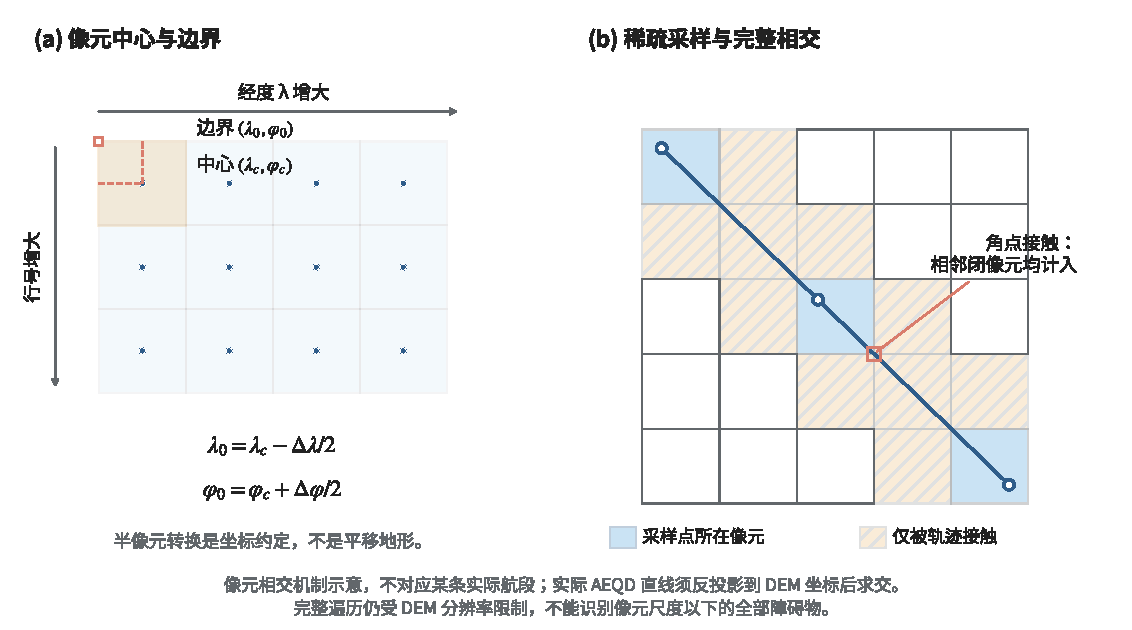
\includegraphics[width=\linewidth]{figures/common_model/figA1_dem_cells.pdf}
\caption{像元中心约定与连续航迹完整相交（机制示意，非真实航段；不识别DEM分辨率以下障碍物）}\label{fig:dem_closed_cells}
\end{figure}

\end{document}
